%% LyX 2.3.6.1 created this file.  For more info, see http://www.lyx.org/.
%% Do not edit unless you really know what you are doing.
\documentclass[twoside,english]{article}
\usepackage[T1]{fontenc}
\usepackage[latin9]{inputenc}
\usepackage{geometry}
\geometry{verbose,tmargin=2cm,bmargin=2cm,lmargin=2cm,rmargin=2cm}
\usepackage{color}
\usepackage{amsmath}
\usepackage{amssymb}

\makeatletter
%%%%%%%%%%%%%%%%%%%%%%%%%%%%%% User specified LaTeX commands.
\usepackage{helvet}
\renewcommand{\familydefault}{\sfdefault}
\usepackage[T1]{fontenc}
\usepackage[latin9]{inputenc}
\usepackage{geometry}
\geometry{verbose,tmargin=1.8cm,bmargin=4cm,lmargin=1.5cm,rmargin=2cm}
\usepackage{enumitem}
\usepackage{amstext}
\usepackage{amsthm}
\usepackage{amssymb}
\usepackage{setspace}
\usepackage{graphicx}
\doublespacing


\usepackage{enumitem}
\setenumerate[1]{label=\textbf{\arabic*}}
\setenumerate[2]{label=\textbf{(\alph*)}}
\setenumerate[3]{label=\textbf{(\roman*)}}
\setlist[enumerate]{align=right}

\setcounter{page}{2}

%for upright integrals
\usepackage[integrals]{wasysym}

%to be used in conjunction with fancyfoot for last page
\usepackage{zref-totpages}

%fancyhrd settings
\usepackage{fancyhdr}
\pagestyle{fancy}
\fancyhf{}

\fancypagestyle{laststyle}
{
   \fancyhf{}
   \chead{\thepage}
   \fancyfoot[L]{\copyright NJC }
   \fancyfoot[R]{\textbf{END}} %Put \thispagestyle{laststyle} in the last page
}

%%centering page number
\chead{\thepage}

\renewcommand{\headrulewidth}{0pt}
\renewcommand{\footrulewidth}{0pt}

%%footer settings, different footer for ODD and EVEN pages, also for the LASTPAGE
\fancyfoot[LO]{Generated with Python Script by BRW\hfill \textbf{[Turn Over}}
\fancyfoot[LE]{Generated with Python Script by BRW }

%%shameless self-plug BRW

\makeatother

\usepackage{babel}
\begin{document}

\begin{enumerate}\item \textbf{{[}ALVL/9597/2013/P1/Q1{]} }

The files \texttt{WORDS1.TXT} and \texttt{WORDS2.TXT} store a list
of single word computing terms used in a textbook.

Each entry has the following format: 

\texttt{<computing term>}

\texttt{<number>}

One of the file entries (in both files) is:

\texttt{program }

\texttt{52}

This means that after a complete scan of the textbook the word 'program'
was found 52 times.

\subsubsection*{Task 1.1}

Write program code to find and output the term with the highest number
of occurrences. Use the file \texttt{WORDS1.TXT} to test your program.

\subsubsection*{Evidence 1}

The program code. \hfill{}{[}8{]}

\subsubsection*{Evidence 2}

Screenshot of output. \hfill{}{[}1{]}

\subsubsection*{Task 1.2}

Amend your program code so that if more than one term exists with
the highest number of occurrences, all terms are reported. Use the
file \texttt{WORDS2.TXT} to test your program.

\subsubsection*{Evidence 3}

The program code. \hfill{}{[}5{]}

\subsubsection*{Evidence 4}

Screenshot of output.\hfill{} {[}1{]}

 \newpage 

\quad{}
\item \textbf{{[}ALVL/9597/2013/P1/Q2{]} }

A company keeps data about its employees. The employee surname and
employee ID are recorded. 

All employee IDs are unique and have the format C999 where C is any
uppercase letter and 9 is a digit.

A program is to be produced to search by either:
\begin{itemize}
\item The surname, which then reports the matching employee ID
\item The employee ID, which then reports the matching surname
\end{itemize}
The programmer stores the data a two 1-dimensional arrays and produces
the following search algorithm to search a string array and output
the matching value from the second array.

\noindent %
\noindent\begin{minipage}[t]{1\columnwidth}%
\texttt{INPUT SearchItem }

\texttt{FOR Index \textleftarrow{} 1 TO UpperBound }

\texttt{\qquad{}IF SearchItem = Array1{[}Index{]} }

\texttt{\qquad{}\qquad{}THEN OUTPUT Array2{[}Index{]} }

\texttt{\qquad{}ENDIF }

\texttt{ENDFOR}%
\end{minipage}

This search algorithm is inefficient.

The programmer uses the following design to produce the program code:
\begin{itemize}
\item code to search by surname 
\item The search algorithm has \texttt{Surname} as \texttt{Array1} and \texttt{EmployeeID}
as \texttt{Array2} followed by code to search by employee ID 
\item The search algorithm has \texttt{EmployeeID} as \texttt{Array1} and
\texttt{Surname} as \texttt{Array2}
\end{itemize}
This design would produce repetition of code.

\subsubsection*{Task 2.1}

Write program code which performs each of the searches:
\begin{itemize}
\item Search by surname 
\item Search by employee ID
\end{itemize}
Your code should address the issues of inefficiency and repetition
of code described in the scenario above. 

Use the sample array data available from the text file \texttt{EMPLOYEEDATA.txt}
and paste this into your program code.

\subsubsection*{Evidence 5}

Your program code.\hfill{} {[}11{]}

\subsubsection*{Task 2.2}

Devise a set of four test cases with the data to be used.

\subsubsection*{Evidence 6}

A screenshot for each test case you considered. Annotate the screenshot
explaining the purpose of each test. \hfill{}{[}4{]}

 \newpage 

\quad{}
\item \textbf{{[}ALVL/9597/2013/P1/Q3{]} }

The task is to store a dataset (maximum size 20 items) as a binary
tree structure. You should assume that the data items are unique.

The program will use a user-defined type Node for each node defined
as follows:
\begin{center}
\begin{tabular}{|l|l|l|}
\hline 
\texttt{\hspace{0.01\columnwidth}}Identifier & \texttt{\hspace{0.01\columnwidth}}Data Type & \texttt{\hspace{0.05\columnwidth}}Description\tabularnewline
\hline 
\texttt{LeftP} & \texttt{INTEGER} & The left pointer for the node\tabularnewline
\hline 
\texttt{Data} & \texttt{STRING} & The node's data value\tabularnewline
\hline 
\texttt{RightP} & \texttt{INTEGER } & The right pointer for the node\tabularnewline
\hline 
\end{tabular}
\par\end{center}

A linked list is maintained of all the unused nodes which do not form
part of the tree. The first available node which is used for a new
term is indicated by NextFreePosition. Items in the unused list are
linked using their left pointers.

The binary tree and linked list are implemented using variables as
follows:
\begin{center}
\begin{tabular}{|l|l|l|}
\hline 
\texttt{\hspace{0.01\columnwidth}}Identifier & \texttt{\hspace{0.01\columnwidth}}Data Type & \texttt{\hspace{0.05\columnwidth}}Description\tabularnewline
\hline 
\texttt{ThisTree} & \texttt{ARRAY{[}20{]} : Node} & The tree data\tabularnewline
\hline 
\texttt{Root } & \texttt{INTEGER} & Index for the root position of the \texttt{ThisTree} array\tabularnewline
\hline 
\texttt{NextFreePosition} & \texttt{INTEGER } & Index for the next unused node\tabularnewline
\hline 
\end{tabular}
\par\end{center}

\begin{center}
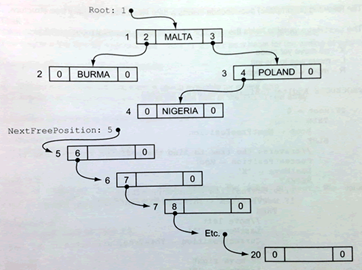
\includegraphics[width=0.5\paperwidth]{C:/Users/Admin/Desktop/Github/question_bank/LyX/static/img/9597-ALVL-2013-P1-Q3}
\par\end{center}

The diagram shows the binary tree and linked list after four values
have been added.

\subsubsection*{Task 3.1}

Write the program code to declare all the required variables and create
the initial linked list which contains all 20 nodes. Add statement(s)
to initialise the empty tree.

\hfill{}{[}10{]}

\subsubsection*{Evidence 7}

Your program code for Task 3.1. {[}11{]}

The following (incomplete) pseudocode inserts a data value into the
binary tree structure.

The \texttt{LastMove} variable holds the direction of the previous
traversal move as follows:

X - no move yet made 

L - move was to the left 

R - move was to the right

\noindent %
\noindent\begin{minipage}[t]{1\columnwidth}%
\texttt{PROCEDURE AddItemToBinaryTree(NewFreeItem)}

\texttt{\qquad{}IF Root = 0}

\texttt{\qquad{}\qquad{}THEN}

\texttt{\qquad{}\qquad{}\qquad{}Root \textleftarrow{} NextFreePosition}

\texttt{\qquad{}\qquad{}ELSE}

\texttt{\qquad{}\qquad{}\qquad{}// traverse the tree to find the
position for the new value}

\texttt{\qquad{}\qquad{}\qquad{}CurrentPosition \textleftarrow{}
Root}

\texttt{\qquad{}\qquad{}\qquad{}LastMove \textleftarrow{} 'X'}

\texttt{\qquad{}\qquad{}\qquad{}REPEAT}

\texttt{\qquad{}\qquad{}\qquad{}\qquad{}PreviousPosition \textleftarrow{}
CurrentPosition}

\texttt{\qquad{}\qquad{}\qquad{}\qquad{}IF NewFreeItem < ThisTree{[}CurrentPosition{]}.Data}

\texttt{\qquad{}\qquad{}\qquad{}\qquad{}\qquad{}THEN}

\texttt{\qquad{}\qquad{}\qquad{}\qquad{}\qquad{}\qquad{}// move
left}

\texttt{\qquad{}\qquad{}\qquad{}\qquad{}\qquad{}\qquad{}LastMove
\textleftarrow{} 'L'}

\texttt{\qquad{}\qquad{}\qquad{}\qquad{}\qquad{}\qquad{}CurrentPosition
\textleftarrow{} ThisTree{[}CurrentPosition{]}.LeftP}

\texttt{\qquad{}\qquad{}\qquad{}\qquad{}\qquad{}ELSE}

\texttt{\qquad{}\qquad{}\qquad{}\qquad{}\qquad{}\qquad{}// move
right}

\texttt{\qquad{}\qquad{}\qquad{}\qquad{}\qquad{}\qquad{}LastMove
\textleftarrow{} 'R'}

\texttt{\qquad{}\qquad{}\qquad{}\qquad{}\qquad{}\qquad{}CurrentPosition
\textleftarrow{} ThisTree{[}CurrentPosition{]}.RightP}

\texttt{\qquad{}\qquad{}\qquad{}\qquad{}ENDIF}

\texttt{\qquad{}\qquad{}\qquad{}UNTIL CurrentPosition = 0}

\texttt{\qquad{}ENDIF}

\texttt{\qquad{}IF LastMove = 'R'}

\texttt{\qquad{}\qquad{}THEN}

\texttt{\qquad{}\qquad{}\qquad{}ThisTree{[}PreviousPosition{]}.RightP
\textleftarrow{} NextFreePosition}

\texttt{\qquad{}\qquad{}ELSE}

\texttt{\qquad{}\qquad{}\qquad{}ThisTree{[}PreviousPosition{]}.LeftP
\textleftarrow{} NextFreePosition}

\texttt{\qquad{}ENDIF}

\texttt{\qquad{}NextFreePosition ThisTree{[}NextFreePosition{]}.LeftP}

\texttt{ENDPROCEDURE}%
\end{minipage}

Note: The above text is available in the text file \texttt{PSEUDOCODE\_TASK\_3\_2.TXT}

\subsubsection*{Task 3.2}

Write non-recursive code to implement the \texttt{AddItemToBinaryTree}
procedure. You may use the text file \texttt{PSEUDOCODE\_TASK\_3\_2.TXT}
as a basis for the writing of your code.

The given pseudocode is incomplete as:
\begin{itemize}
\item it does not initially test that there is space available for a new
item 
\item it does not assign \texttt{NewTreeItem} to the data field of the \texttt{ThisTree}
array
\end{itemize}
Add these requirements to your program solution.

\subsubsection*{Evidence 8}

Your program code for Task 3.2.\hfill{} {[}6{]}

\subsubsection*{Task 3.3}

Write a procedure\texttt{ OutputData} which displays the value of
\texttt{Root}, the value of \texttt{NextFreePosition} and the contents
of \texttt{ThisTree} in index order.

\subsubsection*{Evidence 9}

Your program code for Task 3.3. \hfill{}{[}5{]}

\subsubsection*{Task 3.4}

Write a main program to:
\begin{itemize}
\item Input new data items and add them to the binary tree by calling procedure
\texttt{AddItemToBinaryTree}. The input is terminated with value \textquotedbl\texttt{XXX}\textquotedbl .
Do not attempt to validate the input of the country names. 
\item Your program will then call procedure \texttt{OutputData}.
\end{itemize}
Run the program with the input of the single value \textquotedbl\texttt{XXX}\textquotedbl .

\subsubsection*{Evidence 10}

Screenshot showing the output from running the program in Task 3.4.\hfill{}
{[}3{]}

\subsubsection*{Task 3.5}

Test your program using the following data items input in the order
shown:
\begin{center}
\texttt{INDIA, NEPAL, MALAYSIA, SINGAPORE, BURMA, CANADA, LATVIA,
XXX}
\par\end{center}

\subsubsection*{Evidence 11}

Provide screenshot test evidence for Task 3.5. \hfill{}{[}5{]}

Further program code is required to carry out an \textbf{in-order
traversal}.

\subsubsection*{Task 3.6}

Write a recursive procedure to carry out an in-order tree traversal. 

Include a call to the procedure from your main program.

\subsubsection*{Evidence 12}

Your program code. \hfill{}{[}8{]}

\subsubsection*{Evidence 13}

Produce a screenshot for the Task 3.5 dataset confirming the output
of the countries in alphabetical order. \hfill{}{[}2{]}

 \newpage 

\quad{}
\item \textbf{{[}ALVL/9597/2013/P1/Q4{]} }

The task is to input data for a frequency distribution and then output
to the screen a horizontal bar chart.

The data is input as an X value followed by its frequency. Assume
the frequency is always in the range 0 to 60 and there are no more
than six X values.

The input shown below shows the number of sweatshirts sold in a retail
shop over a one week period; for example there were 39 XL items sold

\noindent\fbox{\begin{minipage}[t]{1\columnwidth - 2\fboxsep - 2\fboxrule}%
\texttt{Next X value ... <ZZZ to END> XS }

\texttt{Frequency ... 12 }

\texttt{Next X value ... <ZZZ to END> S }

\texttt{Frequency ... 22 }

\texttt{Next X value ... <ZZZ to END> M }

\texttt{Frequency ... 45 }

\texttt{Next X value ... <ZZZ to END> L }

\texttt{Frequency ... 56 }

\texttt{Next X value ... <ZZZ to END> XL }

\texttt{Frequency ... 39 }

\texttt{Next X value ... <ZZZ to END> XXL}

\texttt{Frequency ... 11 }

\texttt{Next X value ... <ZZZ to END> ZZZ}

\texttt{++++++++++++++++++++++++++++++++++++++++}

\texttt{Frequency distribution }

\texttt{++++++++++++++++++++++++++++++++++++++++}

\texttt{XS ~@@@@@@@@@@@@ }

\texttt{S ~~@@@@@@@@@@@@@@@@@@@@@@ }

\texttt{M ~~@@@@@@@@@@@@@@@@@@@@@@@@@@@@@@@@@@@@@@@@@@@@@ }

\texttt{L ~~@@@@@@@@@@@@@@@@@@@@@@@@@@@@@@@@@@@@@@@@@@@@@@@@@@@@@@@@ }

\texttt{XL ~@@@@@@@@@@@@@@@@@@@@@@@@@@@@@@@@@@@@@@@ }

\texttt{XXL @@@@@@@@@@@}%
\end{minipage}}

\subsubsection*{Task 4.1}

Write a program which inputs a set of X values and frequencies and
produces output in the format shown.

\subsubsection*{Evidence 14}

Your program code for Task 4.1.\hfill{}{[}8{]}

\subsubsection*{Evidence 15}

A screenshot to confirm the dataset used and the output produced.
\hfill{}{[}2{]}

The appearance of the bar chart display is to be improved as follows:
\begin{itemize}
\item Each bar is to be represented by more than one line of the same character
to that its bar width is increased. 
\item Each bar will be shown with the same number of lines. 
\item The complete bar chart, including the heading, is to take up no more
than 40 lines. 
\item The line width for the output is exactly 80 characters. 
\item Its appearance could be improved by changing the @ character.
\end{itemize}

\subsubsection*{Task 4.2}

Write code to produce a new chart for the data used in Task 4.1 showing
the maximum possible bar width and any other refinements you have
introduced.

\subsubsection*{Evidence 16}

Your program code for Task 4.2. \hfill{}{[}4{]}

\subsubsection*{Evidence 17}

A screenshot showing the data entry followed by the bar chart. \hfill{}{[}2{]}

Some datasets will have a frequency which is greater than 60 and so
the frequencies of the dataset can no longer be shown with a corresponding
number of characters in the line. The frequencies will need to be
scaled before the output is attempted.

The bar chart would benefit by the inclusion of a horizontal axis
labelled with a scale showing the frequency values.

\subsubsection*{Task 4.3}

Revise your program code to meet these new requirements.

\subsubsection*{Evidence 18}

Your program code for Task 4.3.\hfill{} {[}8{]}

\subsubsection*{Evidence 19}

Screenshots demonstrating: 
\begin{itemize}
\item Dataset 1 as used in Task 4.1 which needs no scaling 
\item Dataset 2 of your choice to demonstrate frequencies which must be
scaled 
\item Dataset 3 of your choice to demonstrate frequencies which must be
scaled differently to Dataset 2 
\end{itemize}
\hfill{}{[}6{]}

 \newpage 

\item \textbf{{[}ALVL/9597/2013/P2/Q1{]} }

A dental practice currently uses a computer system to store details
of its patients, staff and appointments in separate files.

The practice manager and the receptionist have their own computers
for accessing and updating the files.

The system produces a small number of reports.

An updated system is to be produced by a software company. The updated
system will use a database. In the updated system the dentists will
be given a hand-held device to use in their rooms for accessing and
updating the patient records. The new system will also be capable
of producing additional reports.

The software company has software engineers who have expert skills
in specific areas of software development. A number of the engineers
will be involved in the development of the updated system.
\begin{enumerate}
\item Describe and justify three methods which can be used to determine
what further reports are required from the updated computer system.
{[}6{]}
\item The work to update the system is partly managed by the following Program
Evaluation and Review Technique (PERT) chart.

A - investigation 

B - analysis 

C - design of database 

D - design of reports 

E - design of screen displays for dentists 

F - transfer of data from files into database 

G - documentation produced 

H - acceptance testing 

I - hand over to customer

Time is measured in weeks.
\begin{center}
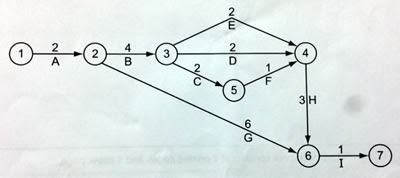
\includegraphics[width=0.5\paperwidth]{C:/Users/Admin/Desktop/Github/question_bank/LyX/static/img/9597-ALVL-2013-P2-Q1-1}
\par\end{center}
\begin{enumerate}
\item State the critical path.\hfill{} {[}1{]}
\item State the minimum time in which the updated system could be operational.
\hfill{}{[}1{]}
\item For activity E state the 
\begin{itemize}
\item earliest Start time 
\item earliest Finish time 
\item latest Start time
\item latest Finish time\hfill{}{[}4{]}
\end{itemize}
\end{enumerate}
\item {}\textcolor{white}{\_}
\begin{center}
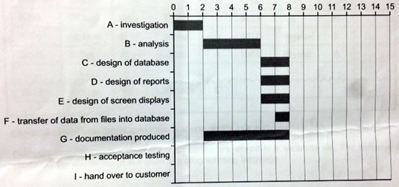
\includegraphics[width=0.5\paperwidth]{C:/Users/Admin/Desktop/Github/question_bank/LyX/static/img/9597-ALVL-2013-P2-Q1-2}
\par\end{center}

The Gantt chart above is based on the information in part \textbf{(b)}.
The timing of two activities is missing and also the timing of one
of the activities shown is incorrect.

Draw a sketch of the Gantt chart to show the correct version. \hfill{}{[}4{]}
\item Explain how the Gantt chart can help with the work that the software
engineers have to carry out. \hfill{}{[}2{]}
\item A small team is put together to consider security aspects of the updated
system.
\begin{enumerate}
\item Identify \textbf{two} possible members of the team and justify your
choice.\hfill{} {[}4{]}
\end{enumerate}
The team have to produce a report to which they all make a contribution.
The report is stored on a network. Each member of the team has access
to allow them to add their contribution.
\begin{enumerate}
\item[ii]  Give \textbf{two} examples of unethical behaviour by a team member.\hfill{}
{[}2{]}
\end{enumerate}
\item Name and describe \textbf{two} types of documentation produced for
this project.\hfill{} {[}6{]}

\noindent\fbox{\begin{minipage}[t]{1\columnwidth - 2\fboxsep - 2\fboxrule}%
End-User documentation 
\begin{itemize}
\item for actual users of system to learn about features and how to use
them 
\item minimum/recommended hardware and software system requirements (operating
system, version, processor, amount of RAM and hard disk space, etc.) 
\item installation guide + step by step guide of how to perform a task or
use a feature 
\item frequently asked questions (FAQ) for common troubleshooting problems
and solutions 
\item support contact information, safety instructions, warranty information
\end{itemize}
Technical documentation
\begin{itemize}
\item for developers to document technical requirements and features of
system
\item system objectives and scope 
\item input and output/report specifications 
\item data storage/database specification 
\item modules/processes and algorithms 
\item user interfaces and application programming interfaces (APIs) 
\item testing
\item implementation/deployment 
\item bugs report and known issues
\end{itemize}
%
\end{minipage}}
\end{enumerate}
The hand-held devices the dentists use in their practice rooms will
be networked. Both client-side scripting and server-side scripting
will be used in the new software which is produced. An intranet with
a web server will be created. Web browsers will be used on the hand-held
devices.
\begin{enumerate}
\item[(g)]  Describe three possible uses of the device.\hfill{} {[}6{]}
\item[(h)]  For each scripting method, client-side scripting and server-side
scripting, give an appropriate example. Justify your response.\hfill{}
{[}4{]}
\end{enumerate}

 \newpage 

\item \textbf{{[}ALVL/9597/2013/P2/Q2{]} }

Examination centres receive examination results for their candidates
as a printed report. The report lists the candidates in order based
on their Index Number. For each candidate their results occupy one
row of the report. Each row displays the results for all subjects
that the candidate sat in the examination.
\begin{center}
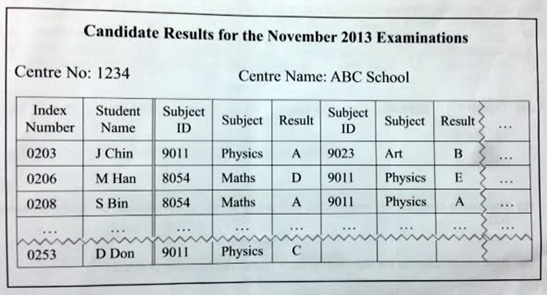
\includegraphics[width=0.5\paperwidth]{C:/Users/Admin/Desktop/Github/question_bank/LyX/static/img/9597-ALVL-2013-P2-Q2-1}
\par\end{center}

Candidates can only take examinations at one centre in a particular
session.

Currently the candidate results for each centre are stored in a separate
file. The software that produces the above report is written in a
programming language.
\begin{enumerate}
\item Describe, using an example, why this file has data redundancy.\hfill{}
{[}2{]}
\item An extra field is added to the file, but the report will not include
this new field. 

Describe the problem that will arise. \hfill{}{[}3{]}
\end{enumerate}
A normalised database solution to this problem is designed, which
has a number of tables.
\begin{enumerate}
\item[(c)]  Draw an E-R diagram that shows these tables and the relationships
between them.\hfill{} {[}5{]}
\item[(d)]  When the data are stored in a database, privacy is of great concern.

Explain why.\hfill{} {[}2{]}
\end{enumerate}

 \newpage 

\item \textbf{{[}ALVL/9597/2013/P2/Q3{]} }

A hash table has an index range of 1 to 900. The following pseudocode
describes an algorithm for searching the table using the hashing function
Hash. It is assumed that the key is present in the table.

\noindent %
\noindent\begin{minipage}[t]{1\columnwidth}%
\texttt{01 Index <- Hash(Key) }

\texttt{02 WHILE Table{[}Index, 1{]} <> Key }

\texttt{03 \qquad{}Index <- Index + 1 }

\texttt{04 ENDWHILE }

\texttt{05 Value <- Table{[}Index, 2{]}}%
\end{minipage}
\begin{enumerate}
\item Explain the purpose of:
\begin{enumerate}
\item line 3
\item line 5\hfill{} {[}4{]}
\end{enumerate}
\item Describe a problem that might occur with a key which, when hashed,
produces an index of 900. \hfill{}{[}2{]}
\item What modification to the algorithm is required to overcome this problem?
\hfill{}{[}3{]}
\item Explain how a new item can be added to this hash table. \hfill{}{[}4{]}
\end{enumerate}

 \newpage 

\item \textbf{{[}ALVL/9597/2013/P2/Q4{]} }

A software development company currently hosts its own email server.
The company is considering a replacement webmail service, using cloud
computing.
\begin{enumerate}
\item (a) State two advantages of this change.\hfill{} {[}2{]}
\item (b) State one disadvantage of this change. \hfill{}{[}1{]}
\end{enumerate}
The company is also considering other uses of the cloud. These include
collaborative activities between employees of the company and also
assistance in developing new software.
\begin{enumerate}
\item[(c)]  Describe an example of how employees of the company may use the
cloud to work collaboratively.\hfill{} {[}3{]}
\item[(d)]  Describe how the cloud can be beneficial to the company when developing
new software for a client. \hfill{}{[}4{]}
\end{enumerate}

 \newpage 

\item \textbf{{[}ALVL/9597/2013/P2/Q5{]} }

Bank customers are allowed to withdraw money from their accounts at
an ATM. They cannot withdraw more than the current balance in their
account. There is a daily limit on the amount that can be withdrawn.
In some circumstances a charge is made for the transaction. The rules
are:
\begin{itemize}
\item the transaction is rejected if the withdrawal amount requested is
greater than the current balance 
\item the transaction is rejected if the withdrawal amount exceeds the daily
limit 
\item if the current balance before the transaction is carried out is less
than 50 dollars then any successful transaction incurs a fixed charge
\end{itemize}
\begin{enumerate}
\item Create a decision table showing all the possible conditions and actions.
\hfill{}{[}4{]}
\item Simplify your decision table by removing redundancies. \hfill{}{[}4{]}
\item Using your answer in (b) write a function using pseudocode. The function
returns:
\begin{itemize}
\item -1 to indicate a rejection; 
\item 0 for a charge-free successful transaction; 
\item the charge for a chargeable successful transaction.\hfill{} {[}5{]}
\end{itemize}
\item State two ways in which your answer in (c) demonstrates clarity of
code. \hfill{}{[}2{]}
\end{enumerate}

 \newpage 

\item \textbf{{[}ALVL/9597/2013/P2/Q6{]} }

The ASCII code for the character 'Z', expressed as a denary integer,
is 90.
\begin{enumerate}
\item Express the denary integer 90 as:
\begin{enumerate}
\item an eight-bit binary number
\item a hexadecimal number \hfill{}{[}2{]}
\end{enumerate}
\item Give two reasons why hexadecimal numbers are used in computing. \hfill{}{[}2{]}
\item State the ASCII code for 'X' in denary. Explain your answer.\hfill{}
{[}2{]}
\item Explain why the Unicode encoding system has replaced ASCII. \hfill{}{[}2{]}
\item Describe a method of storing strings of characters of variable length
in a computer. \hfill{}{[}2{]}
\end{enumerate}

 \newpage 

\item \textbf{{[}ALVL/9597/2019/P1/Q1{]} }

Many applications require the user to search for a data item from
a file or one-dimensional array.

\texttt{JARGON.TXT} is a text file containing computing terms with
one term per line. The program will read all the terms from \texttt{JARGON.TXT}
into an array.

The user will choose if the type of search is to find:
\begin{enumerate}
\item[1.]  An exact match 
\item[2.]  A match at the beginning of the term text
\item[3.]  A match anywhere within the term text
\end{enumerate}

\subsubsection*{Task 1.1}

Design and write program code to:
\begin{itemize}
\item Read the entire contents of \texttt{JARGON.TXT} into an array 
\item Allow the user to repeatedly select the type of search, then input
a term 
\item Output the matching term(s) found 
\item Output a count of the number of matches 
\item End with the input of term \textquotedbl XXX\textquotedbl{}
\end{itemize}
A typical run of the program is shown below:

\texttt{+++++++++++++++++++++++ }

\texttt{1. Exact match }

\texttt{2. Start of term }

\texttt{3. Within term }

\texttt{++++++++++++++++++ }

\texttt{Choice ?1 }

\texttt{Term?firewall }

\texttt{firewall }

\texttt{There were 1 matching term(s)}

\texttt{+++++++++++++++++++++++ }

\texttt{1. Exact match }

\texttt{2. Start of term }

\texttt{3. Within term }

\texttt{++++++++++++++++++ }

\texttt{Choice ?2 }

\texttt{Term?data }

\texttt{data flow diagram }

\texttt{database management system }

\texttt{data file }

\texttt{database }

\texttt{There were 4 matching term(s)}

\texttt{+++++++++++++++++++++++ }

\texttt{1. Exact match }

\texttt{2. Start of term }

\texttt{3. Within term }

\texttt{++++++++++++++++++}

\texttt{Choice ?3 }

\texttt{Term?box }

\texttt{white box testing }

\texttt{black box testing }

\texttt{There were 2 matching term(s)}

\subsubsection*{Evidence 1}

The program code. \hfill{}{[}11{]}

\subsubsection*{Task 1.2}

Study the contents of \texttt{JARGON.TXT} and then design four test
cases to thoroughly test the working of your program code.

\subsubsection*{Evidence 2}

State the test data used in Task 1.2 and show screenshots to confirm
the successful testing of each of your four test cases. \hfill{}{[}4{]}

 \newpage 

\item \textbf{{[}ALVL/9597/2019/P1/Q2{]} }

A binary search (binary chop) is a technique to search for a value
in an ordered dataset.

\subsubsection*{Task 2.1}

Study the identifier table and incomplete recursive algorithm. 

The missing parts of the algorithm are labelled A, B and C.
\begin{center}
\begin{tabular}{|l|c|l|}
\hline 
\texttt{\hspace{0.01\columnwidth}}Variable & \texttt{\hspace{0.01\columnwidth}}Data Type & \texttt{\hspace{0.05\columnwidth}}Description\tabularnewline
\hline 
\texttt{ThisArray} & \texttt{ARRAY OF STRING} & Array containing the the dataset\tabularnewline
\hline 
\texttt{FindValue} & \texttt{STRING} & Item to be found\tabularnewline
\hline 
\texttt{Low} & \texttt{INTEGER} & Lowest index of the considered list\tabularnewline
\hline 
\texttt{High} & \texttt{INTEGER} & Highest index of the considered list\tabularnewline
\hline 
\texttt{Middle} & \texttt{INTEGER} & The array index for the middle position of the current list considered\tabularnewline
\hline 
\end{tabular}
\par\end{center}

\noindent %
\noindent\begin{minipage}[t]{1\columnwidth}%
\texttt{FUNCTION BinarySearch(ThisArray, FindValue, Low, High) RETURNS
INTEGER}

\texttt{\qquad{}DECLARE Middle : INTEGER}

\texttt{\qquad{}IF ............... A ...............}

\texttt{\qquad{}\qquad{}THEN}

\texttt{\qquad{}\qquad{}\qquad{}RETURN -1 // not found}

\texttt{\qquad{}ELSE}

\texttt{\qquad{}\qquad{}// calculate new Middle value}

\texttt{\qquad{}\qquad{}Middle \textleftarrow{} ............... B
...............}

\texttt{\qquad{}\qquad{}IF ThisArray{[}Middle{]} > FindValue}

\texttt{\qquad{}\qquad{}\qquad{}THEN}

\texttt{\qquad{}\qquad{}\qquad{}\qquad{}RETURN BinarySearch(ThisArray,
FindValue, Low, Middle - 1)}

\texttt{\qquad{}\qquad{}\qquad{}ELSE}

\texttt{\qquad{}\qquad{}\qquad{}\qquad{}IF ThisArray{[}Middle{]}
< FindValue}

\texttt{\qquad{}\qquad{}\qquad{}\qquad{}\qquad{}THEN}

\texttt{\qquad{}\qquad{}\qquad{}\qquad{}\qquad{}\qquad{}............... C
...............}

\texttt{\qquad{}\qquad{}\qquad{}\qquad{}\qquad{}ELSE}

\texttt{\qquad{}\qquad{}\qquad{}\qquad{}\qquad{}\qquad{}RETURN
Middle // found at position Middle}

\texttt{\qquad{}\qquad{}\qquad{}\qquad{}ENDIF}

\texttt{\qquad{}\qquad{}ENDIF}

\texttt{\qquad{}ENDIF}

\texttt{ENDFUNCTION}%
\end{minipage}

\subsubsection*{Evidence 3}

What are the three missing lines in this pseudocode? \hfill{}{[}3{]}

\subsubsection*{Task 2.2}

Write a program to implement binary search. 

The program will
\begin{itemize}
\item Call procedure InitialiseAnimals 
\item Input an animal name
\item Use the function BinarySearch 
\item Report whether or now this animal name was found. If found, also output
the index position.
\end{itemize}
The array in the program has identifier \texttt{MyAnimal}. 

Use the dataset given in the file \texttt{ANIMALS.TXT}. You should
paste the contents of this file into your program. The statements
will form the basis of the code for the procedure \texttt{InitialiseAnimals}.

\subsubsection*{Evidence 4}

Program code for Task 2.2 \hfill{}{[}7{]}

\subsubsection*{Evidence 5}

Screenshot to confirm that an animal wich is present in the list was
found with its index position displayed. \hfill{}{[}1{]}

\subsubsection*{Task 2.3}

Amend the program as follows: 

The program must also output the number of function calls carried
out.

\subsubsection*{Evidence 6}

The amended program code. \hfill{}{[}4{]}

\subsubsection*{Evidence 7}

Screenshots showing the amended ouput for runs of the program where: 
\begin{itemize}
\item the animal is found
\item the animal is not found. \hfill{}{[}2{]}
\end{itemize}

 \newpage 

\item \textbf{{[}ALVL/9597/2019/P1/Q3{]} }

A program is to be written to represent and implement a linked list
of nodes. Each node contains a string data value and a pointer. The
pointers link the data items in alphabetical order. 

The unused nodes are linked as shown below. The first unused node
is the position where the next new data item is to be stored. 
\begin{center}
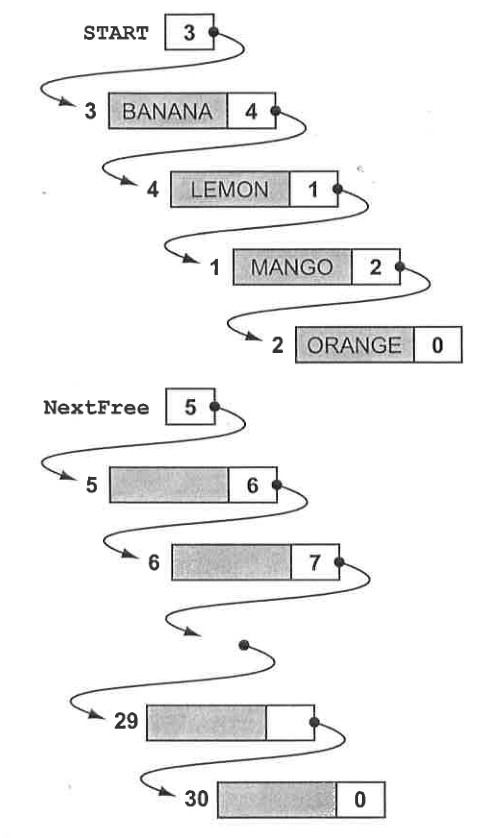
\includegraphics[width=0.25\paperwidth]{C:/Users/Admin/Desktop/Github/question_bank/LyX/static/img/9597-ALVL-2014-P1-Q3}
\par\end{center}

The diagram shows the linked list with: 
\begin{itemize}
\item the items MANGO, ORANGE, BANANA and LEMON (added in that order). 
\item the unused nodes linked together.
\end{itemize}
Each node is implemented as an instance of the class\texttt{ ListNode}.
The class \texttt{ListNode} has the following properties: 
\begin{center}
\begin{tabular}{|l|c|l|}
\hline 
\multicolumn{3}{|c|}{Class\texttt{: ListNode}}\tabularnewline
\hline 
\multicolumn{3}{|c|}{Properties}\tabularnewline
\hline 
\texttt{\hspace{0.01\columnwidth}}Identifier & \texttt{\hspace{0.01\columnwidth}}Data Type & \texttt{\hspace{0.01\columnwidth}}Description\tabularnewline
\hline 
\texttt{DataValue} & \texttt{STRING} & The node data\tabularnewline
\hline 
\texttt{PointerValue} & \texttt{INTEGER} & The node pointer\tabularnewline
\hline 
\end{tabular}
\par\end{center}

A linked list is implemented as an instance of the class \texttt{LinkedList}.
The class \texttt{LinkedList} has the following properties and methods: 
\begin{center}
\begin{tabular}{|l|c|>{\raggedright}p{0.25\columnwidth}|}
\hline 
\multicolumn{3}{|c|}{Class\texttt{: LinkedList}}\tabularnewline
\hline 
\multicolumn{3}{|c|}{Properties}\tabularnewline
\hline 
\texttt{\hspace{0.01\columnwidth}}Identifier & \texttt{\hspace{0.01\columnwidth}}Data Type & \texttt{\hspace{0.01\columnwidth}}Description\tabularnewline
\hline 
\texttt{Node} & \texttt{ARRAY{[}30{]} OF ListNode} & The linked list data structure --- data values and pointers.The array
index starts at 1.For testing purposes the dataset has a maximum of
30 items.\tabularnewline
\hline 
\texttt{Start} & \texttt{INTEGER} & Index position of the node at the start of the linked list\tabularnewline
\hline 
\texttt{NextFree} & \texttt{INTEGER} & Index position of the next unused node \tabularnewline
\hline 
\multicolumn{3}{|l|}{Methods}\tabularnewline
\hline 
\texttt{\hspace{0.01\columnwidth}}Identifier &  & \texttt{\hspace{0.01\columnwidth}}Description\tabularnewline
\hline 
\texttt{Initialise} & \texttt{PROCEDURE} & Sets all the node data values to \textquoteleft empty string\textquoteright .

Set pointers to indicate all nodes are unused and linked.

lnitialise values for \texttt{Start} and \texttt{NextFree}.\tabularnewline
\hline 
\texttt{AddNode} & \texttt{PROCEDURE} & Add a new data item to the linked list.\tabularnewline
\hline 
\texttt{Traversal} & \texttt{PROCEDURE} & Display the data items in order.\tabularnewline
\hline 
\texttt{ReverseTraversal} & \texttt{PROCEDURE} & Display the data items in reverse order.\tabularnewline
\hline 
\texttt{DisplayLinkedList} & \texttt{PROCEDURE} & Display the current state of pointers and the array contents.\tabularnewline
\hline 
\texttt{IsEmpty} & \texttt{FUNCTION RETURNS BOOLEAN} & Tests for empty linked list.\tabularnewline
\hline 
\texttt{IsFull} & \texttt{FUNCTION RETURNS BOOLEAN} & Tests for no unused nodes.\tabularnewline
\hline 
\end{tabular}
\par\end{center}

\subsubsection*{Task 3.1}

Write program code that repeatedly:
\begin{itemize}
\item displays a menu with the following choices: 
\begin{enumerate}
\item[1.]  Add an item 
\item[2.]  Traverse the linked list of used nodes and output the data values 
\item[3.]  Output all pointers and data values 
\item[4.]  Exit 
\end{enumerate}
\item calls an appropriate procedure depending on the user's choice. 
\end{itemize}

\subsubsection*{Evidence 8}

Program code for Task 3.1.\hfill{} {[}5{]}

\subsubsection*{Task 3.2}

Write program code for the classes \texttt{ListNode} and \texttt{LinkedList}
including the \texttt{IsEmpty} method. The code should follow the
specification given. 

Do not attempt to write the methods \texttt{AddNode}, \texttt{Traversal},
\texttt{ReverseTraversal} or \texttt{IsFull} at this stage. 

\subsubsection*{Evidence 9}

Program code for the \texttt{ListNode} and \texttt{LinkedList} classes
(Task 3.2).\hfill{} {[}12{]}

\subsubsection*{Task 3.3}

Write code to create a \texttt{LinkedList} object in the main program.

Run the program and select menu choice 3 to confirm the initial values
of the pointers and data values when the linked list is empty. {[}10{]}

\subsubsection*{Evidence 10}

Screenshot confirming all values after initialisation of the \texttt{LinkedList}
object (Task 3.3). 

\hfill{} {[}3{]}

\subsubsection*{Task 3.4}

Consider the \texttt{AddNode} method. The following algorithm will
add a new data item to the linked list. 

The algorithm uses the variables below:
\begin{center}
\begin{tabular}{|l|c|>{\raggedright}p{0.25\columnwidth}|}
\hline 
\texttt{\hspace{0.01\columnwidth}}Identifier & \texttt{\hspace{0.01\columnwidth}}Data Type & \texttt{\hspace{0.01\columnwidth}}Description\tabularnewline
\hline 
\texttt{NewItem} & \texttt{STRING} & New data item input by the user\tabularnewline
\hline 
\texttt{Found} & \texttt{BOOLEAN} & Flags to \texttt{TRUE} when the position at which to insert the new
item has been found\tabularnewline
\hline 
\texttt{Current} & \texttt{INTEGER} & Current array index position during list traversal\tabularnewline
\hline 
\texttt{Previous} & \texttt{INTEGER} & Previous array index position during list traversal\tabularnewline
\hline 
\texttt{Temp} & \texttt{INTEGER} & Temporary storage of pointer value\tabularnewline
\hline 
\end{tabular}
\par\end{center}

\noindent\fbox{\begin{minipage}[t]{1\columnwidth - 2\fboxsep - 2\fboxrule}%
\texttt{PROCEDURE AddNode }

\texttt{\qquad{}INPUT NewItem }

\texttt{\qquad{}Node{[}NextFree{]}.DataValue <\textemdash{} NewItem }

\texttt{\qquad{}IF Start = 0 }

\texttt{\qquad{}\qquad{}THEN }

\texttt{\qquad{}\qquad{}Start <\textemdash{} NextFree }

\texttt{\qquad{}\qquad{}Temp <\textemdash{} Node{[}NextFree{]}.PointerValue }

\texttt{\qquad{}\qquad{}Node{[}NextFree{]}.PointerValue <\textemdash{}
0 }

\texttt{\qquad{}\qquad{}NextFree <\textemdash{} Temp }

\texttt{\qquad{}ELSE }

\texttt{\qquad{}\qquad{}// traverse the list - starting at Start
to find }

\texttt{\qquad{}\qquad{}// the position at which to insert the new
item }

\texttt{\qquad{}\qquad{}Temp <\textemdash{} Node{[}NextFree{]}.PointerValue }

\texttt{\qquad{}\qquad{}IF NewItem < Node{[}Start{]}.DataValue }

\texttt{\qquad{}\qquad{}\qquad{}THEN }

\texttt{\qquad{}\qquad{}\qquad{}\qquad{}// new item will become
the start of the list }

\texttt{\qquad{}\qquad{}\qquad{}\qquad{}Node{[}NextFree{]}.PointerValue
<\textemdash{} Start }

\texttt{\qquad{}\qquad{}\qquad{}\qquad{}Start <\textemdash{} NextFree }

\texttt{\qquad{}\qquad{}\qquad{}\qquad{}NextFree <\textemdash{}
Temp }

\texttt{\qquad{}\qquad{}\qquad{}ELSE }

\texttt{\qquad{}\qquad{}\qquad{}\qquad{}// the new item is not
at the start of the list }

\texttt{\qquad{}\qquad{}\qquad{}\qquad{}Previous <\textemdash{}
0 }

\texttt{\qquad{}\qquad{}\qquad{}\qquad{}Current <\textemdash{}
Start }

\texttt{\qquad{}\qquad{}\qquad{}\qquad{}Found <\textemdash{} False }

\texttt{\qquad{}\qquad{}\qquad{}\qquad{}REPEAT }

\texttt{\qquad{}\qquad{}\qquad{}\qquad{}\qquad{}IF NewItem <=
Node{[}Current{]}.DataValue }

\texttt{\qquad{}\qquad{}\qquad{}\qquad{}\qquad{}\qquad{}THEN }

\texttt{\qquad{}\qquad{}\qquad{}\qquad{}\qquad{}\qquad{}\qquad{}Node{[}Previous{]}.PointerValue
<\textemdash{} NextFree }

\texttt{\qquad{}\qquad{}\qquad{}\qquad{}\qquad{}\qquad{}\qquad{}Node{[}NextFree{]}.PointerValue
<\textemdash{} Current }

\texttt{\qquad{}\qquad{}\qquad{}\qquad{}\qquad{}\qquad{}\qquad{}NextFree
<\textemdash{} Temp }

\texttt{\qquad{}\qquad{}\qquad{}\qquad{}\qquad{}\qquad{}\qquad{}Found
<\textemdash{} True }

\texttt{\qquad{}\qquad{}\qquad{}\qquad{}\qquad{}\qquad{}ELSE }

\texttt{\qquad{}\qquad{}\qquad{}\qquad{}\qquad{}\qquad{}\qquad{}//
move on to the next node }

\texttt{\qquad{}\qquad{}\qquad{}\qquad{}\qquad{}\qquad{}\qquad{}Previous
<\textemdash{} Current }

\texttt{\qquad{}\qquad{}\qquad{}\qquad{}\qquad{}\qquad{}\qquad{}Current
<\textemdash{} Node{[}Current{]}.PointerValue }

\texttt{\qquad{}\qquad{}\qquad{}\qquad{}\qquad{}ENDIF }

\texttt{\qquad{}\qquad{}\qquad{}\qquad{}UNTIL Found = True OR
Current = 0 }

\texttt{\qquad{}\qquad{}\qquad{}\qquad{}IF Current <\textemdash{}
0 }

\texttt{\qquad{}\qquad{}\qquad{}\qquad{}\qquad{}THEN }

\texttt{\qquad{}\qquad{}\qquad{}\qquad{}\qquad{}\qquad{}Node{[}Previous{]}.PointerValue
<\textemdash{} NextFree }

\texttt{\qquad{}\qquad{}\qquad{}\qquad{}\qquad{}\qquad{}Node{[}NextFree{]}.PointerValue
<\textemdash{} 0 }

\texttt{\qquad{}\qquad{}\qquad{}\qquad{}\qquad{}\qquad{}NextFree
<\textemdash{} Temp }

\texttt{\qquad{}\qquad{}\qquad{}\qquad{}ENDIF }

\texttt{\qquad{}\qquad{}ENDIF }

\texttt{\qquad{}ENDIF }

\texttt{ENDPROCEDURE }

Note: The above pseudocode is available in the text file \texttt{PSEUDOCODE\_TASK\_3\_4.TXT}%
\end{minipage}}

Write code to implement for the \texttt{LinkedList} class: 
\begin{itemize}
\item the \texttt{AddNode} method 
\item the \texttt{IsFull} method. 
\end{itemize}
You may use the text file \texttt{PSEUDOCODE\_TASK\_3\_4.TXT} as a
basis for the writing of your code. 

The main program should check each time that the \texttt{LinkedList}
object is not full before using the \texttt{AddNode} method. 

Run the program as follows: 
\begin{itemize}
\item Menu choice 1 four times, inputting the data values: 

MANGO, ORANGE. BANANA. LEMON in that order. 
\item Menu choice 3 to display. 
\end{itemize}

\subsubsection*{Evidence 11}

Program code for method \texttt{AddNode}. \hfill{}{[}8{]}

\subsubsection*{Evidence 12}

Screenshot showing the pointers and the addition of the four nodes
to the linked list.\hfill{} {[}3{]}

\subsubsection*{Task 3.5}

Write program code to implement the \texttt{LinkedList} class method
\texttt{Traversal} by calling the \texttt{TraversalInOrder} procedure
given below. 

\noindent %
\noindent\begin{minipage}[t]{1\columnwidth}%
\texttt{PROCEDURE TraversalInOrder(Index)}

\texttt{\qquad{}IF Index <> 0}

\texttt{\qquad{}\qquad{}THEN}

\texttt{\qquad{}\qquad{}\qquad{}OUTPUT Node{[}lndex{]}.DataValue}

\texttt{\qquad{}\qquad{}\qquad{}// follow the pointer to the next
data item in the linked list}

\texttt{\qquad{}\qquad{}\qquad{}TraversalInOrder(Node{[}Index{]}.PointerValue)}

\texttt{\qquad{}ENDIF}

\texttt{ENDPRCCEDURE}%
\end{minipage}

\subsubsection*{Evidence 13}

Program code for procedures \texttt{Traversal} and \texttt{TraversalInOrder}.\hfill{}
{[}2{]}

\subsubsection*{Task 3.6}

Run the program as follows: 
\begin{itemize}
\item Menu choice 1 four times, inputting the data values: 

MANGO, ORANGE, BANANA. LEMON in that order. 
\item Menu choice 2 to display. 
\end{itemize}

\subsubsection*{Evidence 14}

Screenshot showing the program execution to test the \texttt{Traversal}
method. \hfill{}{[}2{]}

\subsubsection*{Task 3.7}

Make a copy of the \texttt{TraversalInOrder} and \texttt{Traversal}
procedures.

Paste to form two new procedures \texttt{TraversalInReverseOrder}
and \texttt{ReverseTraversal}. 

Make the necessary changes/additions to these procedures in order
that the data items are output in reverse order by calling the new
method \texttt{ReverseTraversal}.

Run the program code from a new menu choice 4.

Test the method using the four items given in Task 3.6.

\subsubsection*{Evidence 15}

Program code for the new procedures. \hfill{}{[}2{]}

\subsubsection*{Evidence 16}

Screenshot showing option 4 selected and the resulting output. \hfill{}{[}1{]}

 \newpage 

\item \textbf{{[}ALVL/9597/2019/P1/Q4{]} }

Design and code a computer program to simulate the following: 

A garden has a rectangular fish pond measuring 15 metres by 8 metres. 

The pond is to be represented on the screen by a rectangular grid.
Each square metre of the pond is represented by an x-coordinate and
a y-coordinate. The top left square metre of the pond display has
x = 1 and y = 1. 

A boy throws a stone into the pond. The user will input the x-coordinate
and y-coordlnate of the stone impact position. 

A grid representing the pond is then displayed with the stone's impact
position: 

\texttt{X coordinate <1 to 15>? 9 }

\texttt{Y coordinate <1 to 8>? 3 }

\texttt{. . . . . . . . . . . . . . . }

\texttt{. . . . . . . . . . . . . . .}

\texttt{. . . . . . . . S . . . . . .}

\texttt{. . . . . . . . . . . . . . .}

\texttt{. . . . . . . . . . . . . . .}

\texttt{. . . . . . . . . . . . . . .}

\texttt{. . . . . . . . . . . . . . .}

\texttt{. . . . . . . . . . . . . . .}

\subsubsection*{Task 4.1}

The following are the suggested characters to use for the visual representation
of the pond: 
\begin{center}
\begin{tabular}{|c|c|l|}
\hline 
Character & ASCII code (decimal) & \texttt{\hspace{0.01\columnwidth}}Represents\tabularnewline
\hline 
. & 46 & One square metre of water\tabularnewline
\hline 
S & 83 & Stone impact position\tabularnewline
\hline 
\end{tabular}
\par\end{center}

Decide on the design to be used for: 
\begin{itemize}
\item The data structure to represent the grid
\item The contents of each square metre of the pond 
\item Procedure(s) and/or function(s)s to be used 
\end{itemize}

\subsubsection*{Evidence 17}

Show your program design (Task 4.1). \hfill{} {[}6{]}

\subsubsection*{Task 4.2}

Write program code to display the pond contents after a single stone
has been thrown. 

\subsubsection*{Evidence 18}

The program code. \hfill{} {[}7{]}

\subsubsection*{Evidence 19}

Screenshot for a single run of the program. \hfill{} {[}1{]}

\subsubsection*{Task 4.3}

The boy has been told to stop throwing stones into the pond because
the pond now has three fish. The fish randomly swim around. Each fish
will occupy a unique grid position.

Using a random number generator, simulate the positioning of the three
fish. 

Use the following character for a fish: 
\begin{center}
\begin{tabular}{|c|c|l|}
\hline 
Character & ASCII code (decimal) & \texttt{\hspace{0.01\columnwidth}}Represents\tabularnewline
\hline 
F & 70 & Fish\tabularnewline
\hline 
\end{tabular}
\par\end{center}

Write program code to show the pond containing the three fish at a
particular instance of time. The program will now only display the
pond and fish. 

\subsubsection*{Evidence 20}

The program code for Task 4.3. \hfill{} {[}6{]}

\subsubsection*{Evidence 21}

Screenshot for a single run of the program. \hfill{} {[}1{]}

\subsubsection*{Task 4.4}

The boy has been asked to feed the fish. He cannot see the fish in
the pond. He throws a food pellet into the pond which lands inside
one of the square metres. If one of the fish is in this square. it
eats the food and becomes a happy fish. 

Use character symbols for the pond\textquoteleft s grid display as
follows: 
\begin{center}
\begin{tabular}{|c|c|l|}
\hline 
Character & ASCII code (decimal) & \texttt{\hspace{0.01\columnwidth}}Represents\tabularnewline
\hline 
. & 46 & One square metre of water\tabularnewline
\hline 
P & 80 & Pellet (if not eaten by one of the fish)\tabularnewline
\hline 
H & 72 & Happy (fed) fish\tabularnewline
\hline 
F & 70 & Fish\tabularnewline
\hline 
\end{tabular}
\par\end{center}

Write program code to simulate the boy throwing one food pellet into
the pond. The user will input an x-coordinate and y-coordinate for
the food pellet position. You should consider the possible reuse of
any code from Tasks 4.2 and 4.3.

\subsubsection*{Evidence 22}

The program code.\hfill{} {[}6{]}

\subsubsection*{Evidence 23}

Screenshotevldence similar to that shown which shows: 
\begin{itemize}
\item one throw which did not feed a fish 

\texttt{X coordinate <1 to 15>? 2 }

\texttt{Y coordinate <1 to 8>? 5 }

\texttt{. . . . . . . . . . . . . . . }

\texttt{. . . . . . . . . . . . . . .}

\texttt{. . . . . . . . F . . . . . .}

\texttt{. . . . . . . . . . . . . . .}

\texttt{. P . . . . . . . . F . . . .}

\texttt{. . . . . . . . . . . . . . .}

\texttt{. . . . F . . . . . . . . . .}

\texttt{. . . . . . . . . . . . . . .}
\item a second throw where a fish was fed 

\texttt{X coordinate <1 to 15>? 1 }

\texttt{Y coordinate <1 to 8>? 5 }

\texttt{. . . . . . . . . . . . . . . }

\texttt{. . . . . . . . . . . . . . .}

\texttt{. . . . . . . . . . . . . . F}

\texttt{. . . . . . . . . . . . . . .}

\texttt{H . . . . . . . . . . . . . .}

\texttt{. . . . . . . . . . . . . . .}

\texttt{. . . . . . . F . . . . . . .}

\texttt{. . . . . . . . . . . . . . .}\hfill{} {[}3{]}
\end{itemize}

 \newpage 

\item \textbf{{[}ALVL/9597/2019/P2/Q1{]} }

A supermarket chain wants to encourage customers to return to its
store. They operate a scheme of rewards for customers based on how
much they spend over a period of time.

Customers are issued with a card that is readable by a Point of Sale
(POS) terminal. When a customer provides their card at the checkout,
the system identifies them and stores the products they purchased
and how much they spent.

Currently the only use of this data is to issue the customer with
vouchers every three months. Vouchers have a value based on the total
amount the customer has spent during the previous three months. The
vouchers can only be used in part payment for goods bought in the
supermarket.

The supermarket managers want to make more use of the customer purchase
data. They hire a software development company to produce software
that will implement new uses of the data.

Software developers have skills in developing software. The supermarket
managers have in depth knowledge of their business. At first, software
developers will have little knowledge of the business.
\begin{enumerate}
\item Explain how the supermarket managers can communicate to the software
developers what they require. \hfill{}{[}2{]}
\item Before designing the new software, the software developers need to
understand the content and structure of the customer purchase data.
Give two methods that can be used for this task, justifying the use
of each. \hfill{}{[}4{]}
\item Once the analysis phase has been completed, describe what decisions
software developers need to make before coding can begin. \hfill{}{[}6{]}
\end{enumerate}
The work to implement new uses of the customer data needs to be managed.
The following Program Evaluation and Review Technique (PERT) chart
is used as a management tool.

Time is measured in weeks. 
\begin{center}
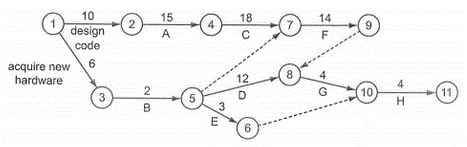
\includegraphics[width=0.7\paperwidth]{C:/Users/Admin/Desktop/Github/question_bank/LyX/static/img/9597-ALVL-2014-P2-Q1}
\par\end{center}
\begin{enumerate}
\item[(d)]  Each activity indicated by a dashed line on the PERT chart is a
dummy activity.
\begin{enumerate}
\item Explain the nature and purpose of a dummy activity.\hfill{} {[}2{]}
\item Each of the following activities matches one of the labels A-H on
the chart.
\begin{itemize}
\item write user documentation 
\item train users 
\item write code 
\item convert files
\item test code 
\item end-user testing 
\item test system 
\item install new hardware
\end{itemize}
Copy and complete the following table, 
\begin{center}
\begin{tabular}{|c|>{\centering}p{0.5\columnwidth}|}
\hline 
Label & Activity\tabularnewline
\hline 
A & \tabularnewline
\hline 
B & \tabularnewline
\hline 
C & \tabularnewline
\hline 
D & \tabularnewline
\hline 
E & \tabularnewline
\hline 
F & \tabularnewline
\hline 
G & \tabularnewline
\hline 
H & \tabularnewline
\hline 
\end{tabular}
\par\end{center}

\hfill{}{[}4{]}
\item Explain the significance of the dummy activity that leads into event
8. \hfill{}{[}3{]}
\end{enumerate}
\item[(e)]  From the PERT chart:
\begin{enumerate}
\item State the critical path.\hfill{} {[}1{]}
\item State the minimum time in which the new software can be developed
and implemented.\hfill{} {[}1{]}
\item The chart omits an activity: \textbf{write technical documentation}.
State a starting point and a finishing point for this activity. Justify
your choices. \hfill{}{[}4{]}
\end{enumerate}
\end{enumerate}
Management staff can already access the company network remotely for
other software applications. Management are to be given the facility
to access, and interact with, the customer data Via the company LAN.
However, a decision is made not to allow access to the customer data
remotely for this updated system.
\begin{enumerate}
\item[(f)]  Describe \textbf{two} methods which can be used to ensure that there
is no remote access to customer data by management staff. \hfill{}{[}4{]}
\end{enumerate}
ln the new system, customers will have access to information through
a web browser. Each customer will be able to see some information
about their purchase history.
\begin{enumerate}
\item[(g)]  Explain what software needs to be developed to provide this customer
facility. \hfill{}{[}5{]}
\item[(h)]  One of the software developers has the task of ensuring that social
issues are considered. This developer has to document these issues. 

Describe \textbf{two} issues that might be in the document with regard
to customers accessing their data. \hfill{}{[}4{]}
\end{enumerate}

 \newpage 

\item \textbf{{[}ALVL/9597/2019/P2/Q2{]} }

Consider the following binary tree:
\begin{center}
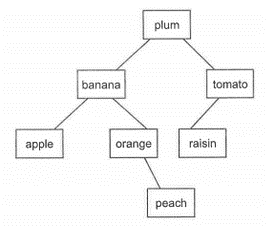
\includegraphics[width=0.35\paperwidth]{C:/Users/Admin/Desktop/Github/question_bank/LyX/static/img/9597-ALVL-2014-P2-Q2}
\par\end{center}
\begin{enumerate}
\item List the nodes, in order, that are visited for a post-order traversal.
\hfill{}{[}2{]}
\item List the nodes, in order, that are visited for an inorder traversal.
\hfill{}{[}2{]}
\item What property is exhibited by the list of items produced in \textbf{part
(b)}? \hfill{}{[}1{]}
\item Describe an algorithm, using pseudocode, to perform a binary tree
search. The output should state whether or not the item is present
in the tree. \hfill{}{[}5{]}
\end{enumerate}

 \newpage 

\item \textbf{{[}ALVL/9597/2019/P2/Q3{]} }

A network manager for a sales company types the following into his
computer:

\texttt{copy C:\textbackslash monthlysales\textbackslash{*}.dat
E\textbackslash :\textbackslash backup\textbackslash junesales
/V}
\begin{enumerate}
\item State the type of user interface being used. \hfill{}{[}1{]}
\item Describe, using the example, two benefits of the user interface named
in \textbf{(a)}. \hfill{}{[}4{]}
\end{enumerate}
The network manager has a disabled user who cannot use a keyboard
but can control a point-and-click device that moves a pointer on the
screen.
\begin{enumerate}
\item[(c)]  Describe a user interface that would allow this user to enter text
into a word processor. \hfill{}{[}3{]}
\item[(d)]  The sales company provides a special user interface for this user.
State\textbf{ two} benefits to the company. \hfill{}{[}2{]}
\end{enumerate}

 \newpage 

\item \textbf{{[}ALVL/9597/2019/P2/Q4{]} }

A small local area network (LAN) in a school consists of one switch,
one file server and ten computers.
\begin{enumerate}
\item Explain why circuit switching could be used in this LAN. \hfill{}{[}2{]}
\end{enumerate}
The network has a connection to the lnternet added.
\begin{enumerate}
\item[(b)] Explain how packet switching is used when a web page is downloaded
from the Internet. \hfill{}{[}3{]}
\end{enumerate}
A packet from the web server consists of 256 bytes. One of the bytes
is the checksum byte. In each byte one bit is the parity bit.
\begin{enumerate}
\item[(c)]  If the byte 0 0 1 1 0 1 0 1 results in a parity error, state the
type of parity being used. \hfill{}{[}1{]}
\item[(d)]  The receiving computer uses the checksum byte to check whether the
packet contains an error. Explain how it does this.\hfill{} {[}4{]}
\end{enumerate}

 \newpage 

\item \textbf{{[}ALVL/9597/2019/P2/Q5{]} }

A software developer is given the task of producing software for a
college. The software will help to manage information about what students
do after finishing at the college.

The destination of each student after college is classified in one
of three possible ways:
\begin{itemize}
\item University
\item Employment 
\item Other
\end{itemize}
The college wishes to store:
\begin{itemize}
\item name 
\item number of A Level passes 
\item destination (U / E / O) 
\item university attended 
\item main subject studied at university 
\item type of employment 
\item what students do when their destination is classified as 'O'
\end{itemize}
The software developer will use an objectoriented approach to developing
a solution.
\begin{enumerate}
\item Draw a class diagram which exhibits the following:
\begin{itemize}
\item suitable classes with appropriate properties and methods 
\item inheritance 
\item polymorphism \hfill{}{[}6{]}
\end{itemize}
\item Explain how your solution to (a) demonstrates software reuse.\hfill{}
{[}2{]}
\end{enumerate}
The data on the students is to be stored in a serial text file called
STUDENT.DAT. Each line of the file has the same structure:

\texttt{<Name><NoOfPasses><Destination><University><MainSubject><EmpType><Other>}

with the string NULL stored where appropriate.
\begin{enumerate}
\item[(c)]  Write an algorithm, in pseudocode, to read data from \texttt{STUDENT.DAT}
and to output the following:
\begin{itemize}
\item total number of students going to university 
\item average number of passes for the students going to university e total
number of students\hfill{} {[}7{]}
\end{itemize}
\end{enumerate}

 \newpage 

\item \textbf{{[}ALVL/9597/2019/P2/Q6{]} }

A function is to be written that returns the sum of all values held
in an array that are greater than a minimum value. The function will
be used with arrays of varying size, but never more than a maximum
of 50 000 elements.

A first attempt at writing the program code for the function is given
below:

\noindent %
\noindent\begin{minipage}[t]{1\columnwidth}%
\texttt{01 FUNCTION TotalSum(Results : ARRAY{[}50000{]} OF REAL, ArraySize
: INTEGER, MinValue : REAL) RETURNS REAL }

\texttt{02 \qquad{}DECLARE Sum, Counter : INTEGER }

\texttt{03 \qquad{}DECLARE Temp : Real }

\texttt{04 \qquad{}Sum = 0.0 }

\texttt{05 \qquad{}\qquad{}FOR Counter = 1 TOO ArraySize }

\texttt{06 \qquad{}\qquad{}\qquad{}Temp = Results{[}Counter{]} }

\texttt{07 \qquad{}\qquad{}\qquad{}IF Temp > MinValue THEN Sum
= Sum {*} Temp }

\texttt{08 \qquad{}\qquad{}ENDEOR }

\texttt{09 \qquad{}RETURN Sum }

\texttt{10 ENDFUNCTION}%
\end{minipage}

The function is included in a program specifically written to test
the function. The main program outputs the value returned by the function.
A compiler was used to compile the source program.
\begin{enumerate}
\item The compiler reported an error at line 5 in the function. Identify
the error and explain why it was flagged as a syntax error. \hfill{}{[}2{]}
\item The compiler also reported an error at line 8. State the type of error
reported by the compiler justifying your answer. \hfill{}{[}2{]}
\end{enumerate}
The errors indicated in \textbf{parts (a)} and \textbf{(b)} were corrected.
A successful compilation produces executable code. When the code was
executed, the program failed to complete and reports an error at line
7.
\begin{enumerate}
\item[(c)]  {} 
\begin{enumerate}
\item State the type of error that occurred. Justify your answer. \hfill{}{[}2{]}
\item The error described in \textbf{part (c) (i)} depends on the detection
of another type of error. Name this other type of error. How should
the code be changed to correct this error?\hfill{}{[}2{]}
\end{enumerate}
\end{enumerate}
When the program finally runs without error, the test plan needs to
be completed. The test plan uses data that tests different sizes of
array, different array values and different minimum values. 

The array \texttt{TempArray} is used in the main program as the array
to be processed.\quad{} 
\begin{enumerate}
\item[(d)]  Each element of \texttt{TempArray} stores a random value between
1.0 and 10.0.
\begin{enumerate}
\item Explain why the function call:

\texttt{TotalSum(TempArray, 1000, 5.0)}

is not an appropriate black box test. \hfill{}{[}2{]}
\item Explain why the function call:

\texttt{TotalSum(TempArray, 10, 10.5)}

is not an appropriate white box test. \hfill{}{[}2{]}
\end{enumerate}
\item[(e)] if each element of \texttt{TempArray} stores the value 1.0, state
a function call that will be an appropriate black box test. Justify
your answer. \hfill{}{[}3{]}
\end{enumerate}

 \newpage 

\item \textbf{{[}ALVL/9597/2015/P1/Q1{]} }

The file \texttt{ADMISSIONS-DATA.TXT} contains the daily total admissions
to a theme park over a period of 50 days. 

The task is to read the numbers from the file and display a sorted
list. 

You will program two different sort algorithms: 
\begin{enumerate}
\item A bubble sort. 
\item Either a quick sort or an insertion sort but not both. 
\end{enumerate}
Task 1.1

Write code for a procedure to display a menu with the following options: 
\begin{center}
\noindent\ovalbox{\begin{minipage}[t]{1\columnwidth - 2\fboxsep - 0.8pt}%
\begin{enumerate}
\item[1]  Read file data
\item[2] Bubble sort
\item[3] Quick sort/ Insertion sort
\item[4] End Task
\end{enumerate}
%
\end{minipage}}
\par\end{center}

\subsubsection*{Task 1.2}

Write the program code for a procedure to implement menu option 1.

\subsubsection*{Evidence 1}
\begin{itemize}
\item The program code for the menu. 
\item Program code for menu option 1. \hfill{}{[}5{]} 
\end{itemize}
Options 2 and 3 will sort and display the sorted data. The algorithm
for a bubble sort is given in file \texttt{BUBBLE.TXT}. 

Write program code as a procedure to implement the bubble sort. 

\subsubsection*{Evidence 2}
\begin{itemize}
\item The bubble sort code procedure. \hfill{}{[}1{]}
\end{itemize}
Write program code as a procedure to implement the quick sort or the
insertion sort. 

\subsubsection*{Evidence 3}
\begin{itemize}
\item Indicate the sort method used.
\item The program for the sort method used. \hfill{}{[}4{]}
\end{itemize}


\subsubsection*{Task 1.3}

Additional code is to be written for each sort procedure. The sort
methods will count and display the number of comparisons made in completing
the sort process. This will provide an indicator of the efficiency
of each algorithm.

Write the additional code to count and display the number of comparisons
made for each sort method.

\subsubsection*{Evidence 4}
\begin{itemize}
\item The output from menu option 2. \hfill{} {[}2{]}
\end{itemize}

\subsubsection*{Evidence 5}
\begin{itemize}
\item The output from menu option 3. \hfill{} {[}2{]}
\end{itemize}

 \newpage 

\item \textbf{{[}ALVL/9597/2015/P1/Q2{]} }

The pseudocode procedure below is given a denary number. The procedure
then outputs the binary equivalent of the denary number.

\noindent %
\noindent\begin{minipage}[t]{1\columnwidth}%
\texttt{PROCEDURE Converter(DenaryNumber : INTEGER) }

\texttt{\qquad{}IF DenaryNumber = 0 OR DenaryNumber = 1 }

\texttt{\qquad{}\qquad{}THEN }

\texttt{\qquad{}\qquad{}\qquad{}OUTPUT DenaryNumber }

\texttt{\qquad{}\qquad{}ELSE }

\texttt{\qquad{}\qquad{}\qquad{}OUTPUT DenaryNumber MOD 2 }

\texttt{\qquad{}\qquad{}\qquad{}Converter(DenaryNumber DIV 2) }

\texttt{\qquad{}ENDIF }

\texttt{ENDPROCEDURE}%
\end{minipage}

\subsubsection*{Task 2.1}

Write program code to implement the given procedure. 

Execute the procedure using 56 as the parameter. 

\subsubsection*{Evidence 6}
\begin{itemize}
\item Program code. 
\item Screenshot showing the output. \hfill{}{[}6{]}
\end{itemize}

\subsubsection*{Task 2.2}

There is an error with the given algorithm. 

Describe the error and the effect it created on the output in Evidence
6. 

\subsubsection*{Evidence 7}
\begin{itemize}
\item Statement(s) to answer Task 2.2. \hfill{}{[}1{]}
\end{itemize}

\subsubsection*{Task 2.3}

Make changes to the procedure Converter which will correct the error. 

Draw up a list of test cases for the testing of the amended code.
by completing a table with the following headings: 
\begin{center}
\begin{tabular}{|l|l|l|}
\hline 
\texttt{DenaryNumber} & Purpose of the test & Expected output\tabularnewline
\hline 
 &  & \tabularnewline
\hline 
$\vdots$ & $\vdots$ & $\vdots$\tabularnewline
\hline 
 &  & \tabularnewline
\hline 
\end{tabular}
\par\end{center}

\subsubsection*{Evidence 8}
\begin{itemize}
\item The amended PROCEDURE Converter program code.
\item The completed table. 
\item Screenshots for two of the tests. \hfill{}{[}11{]}
\end{itemize}

 \newpage 

\item \textbf{{[}ALVL/9597/2015/P1/Q3{]} }

When buying software. the purchaser is issued with a licence key.
The product licence can be purchased for either one or three computers.
A file is maintained of all the licence keys currently active and
whether the licence was for a single-user or 3-users.

The licence key is a 10 character code as follows: 
\begin{center}
\texttt{CCCCCCCCCD }
\par\end{center}
\begin{itemize}
\item \texttt{C} = a randomly generated uppercase letter. 
\item \texttt{D} = a check digit character calculated from the preceding
nine letters.
\end{itemize}
A new licence key is generated for each purchase. 

An example key is produced as follows: 
\begin{itemize}
\item randomly generated letters: \texttt{FGKWRDFTA} 
\item a set of products is calculated as shown: 
\begin{center}
\begin{tabular}{|>{\centering}p{0.1\columnwidth}|>{\centering}p{0.1\columnwidth}|c|c|}
\hline 
Randomly generated letter & ASCII code & Multiplier & Product\tabularnewline
\hline 
\texttt{F} & 70 & 1 & 70\tabularnewline
\hline 
\texttt{G} & 71 & 2 & 142\tabularnewline
\hline 
\texttt{K} & 75 & 3 & 225\tabularnewline
\hline 
\texttt{W} & 87 & 4 & 348\tabularnewline
\hline 
\texttt{R} & 82 & 5 & 410\tabularnewline
\hline 
\texttt{D} & 68 & 6 & 408\tabularnewline
\hline 
\texttt{F} & 70 & 7 & 490\tabularnewline
\hline 
\texttt{T} & 84 & 8 & 672\tabularnewline
\hline 
\texttt{A} & 65 & 9 & 585\tabularnewline
\hline 
\end{tabular}
\par\end{center}
\item Then the total of the products is calculated:
\begin{center}
\begin{tabular}{|c|c|}
\hline 
Total & 3350\tabularnewline
\hline 
\end{tabular}
\par\end{center}
\item The total 3350 is then divided by 11 to give remainder 6. which becomes
the check digit character. 
\item This gives the complete licence key: \texttt{FGKWRDFTA6 }
\item If the calculation gives remainder 10, the check digit character used
is \texttt{X}.
\end{itemize}

\subsubsection*{Task 3.1}

Design a function \texttt{LicenceKey} to generate a new licence key. 

Write program code to implement the function. 

Test the function for \textbf{three} new licence keys. 

\subsubsection*{Evidence 9}
\begin{itemize}
\item Program code for the \texttt{LicenceKey} function. 
\item Screenshot(s) showing the generation of the three new licence keys.
\hfill{}{[}10{]}
\end{itemize}

\subsubsection*{Task 3.2}

A file \texttt{LICENCE-KEYS.TXT} is maintained storing all licence
keys which are currently active. This test file has 20 licence records.You
will need this file for the programming which follows. 

Typical data for two licences are shown: 

\texttt{SYNCTKMMF8 1}

indicates this is a single-user licence. 

\texttt{SNPHHUATV7 3 1} 

purchased as a 3-user licence. but currently has only one registered
user. 

Write program code for a menu with the following options: 
\begin{center}
\noindent\ovalbox{\begin{minipage}[t]{1\columnwidth - 2\fboxsep - 0.8pt}%
\begin{enumerate}
\item[1]  Purchase of a new licence for either a single-user or a 3-user licence
\item[2] Register an additional user to an active 3-user licence
\item[3] End
\end{enumerate}
%
\end{minipage}}
\par\end{center}

\subsubsection*{Task 3.3}

Write code as a procedure for menu option 1.

The requirement will be: 
\begin{itemize}
\item input from the user the type of licence.
\item Generate the new licence key. 
\item Display licence key issued.
\item Save the data as a new record in the \texttt{LICENCE-KEYS.TXT} file. 
\item Display final contents of \texttt{LICENCE-KEYS.TXT} file. 
\end{itemize}

\subsubsection*{Evidence 10}
\begin{itemize}
\item Program code for menu option 1. 
\item Screenshot(s). showing evidence for the issue of the two types of
licence, displaying: 
\begin{itemize}
\item the licence key issued 
\item the final contents of \texttt{LICENCE-KEYS.TXT} file. \hfill{}{[}6{]}
\end{itemize}
\end{itemize}

\subsubsection*{Task 3.4}

Program menu option 2.

Carry out three relevant tests.

\subsubsection*{Evidence 11}
\begin{itemize}
\item Program code for menu option 2.
\item Screenshot evidence of three test cases. \hfill{}{[}5{]}
\end{itemize}
When a licence is purchased, the licence key, licence type (single-user
or 3-user), purchase date and name of the purchaser are recorded. 

A registration process then follows for each computer. 
\begin{itemize}
\item The computer to which a licence is registered has its MAC address
and the date of registration recorded. 
\end{itemize}
The program design to manage purchases and registrations is to be
implemented with object-oriented programming with the following three
classes: 
\begin{center}
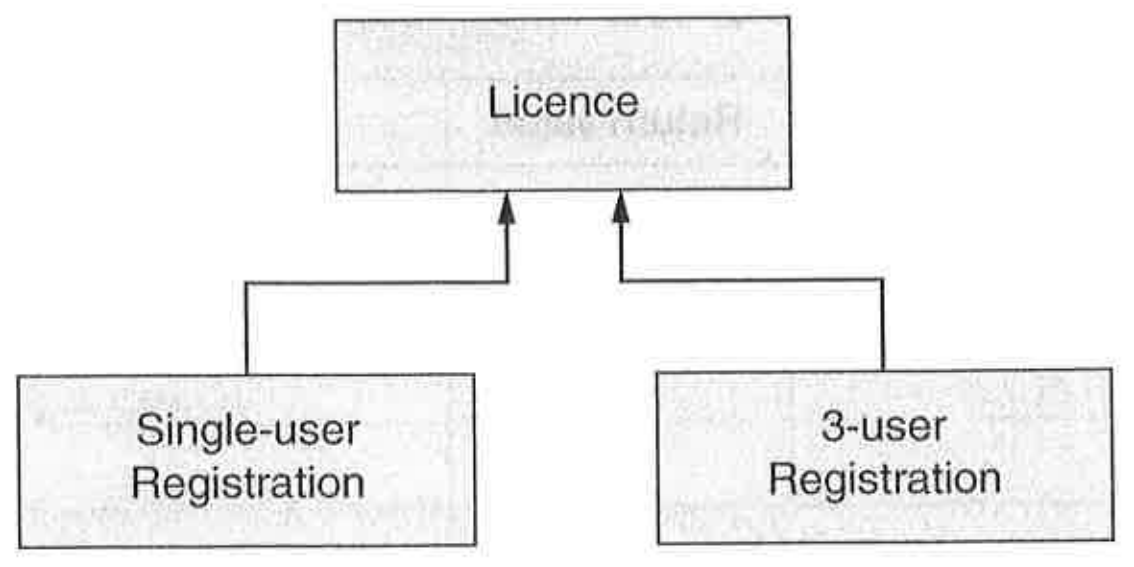
\includegraphics[width=0.5\paperwidth]{C:/Users/Admin/Desktop/Github/question_bank/LyX/static/img/9597-ALVL-2015-P1-Q3}
\par\end{center}

\subsubsection*{Task 3.5}

Write program code \textbf{only} for the three classes shown. 

Do not attempt to develop the application further.

\subsubsection*{Evidence 12}
\begin{itemize}
\item Program code for the three classes.\hfill{}{[}9{]}
\end{itemize}

 \newpage 

\item \textbf{{[}ALVL/9597/2015/P1/Q4{]} }

Users of a local area network each have a network account ID. The
IDs have the format 2015\_NNNN. where N is a digit. 

\subsubsection*{Task 4.1}

Complete the test case table with the addition of \textbf{three} more
invalid User IDs. The reasons for their invalidity should be different. 

The return value is a code as follows: 
\begin{itemize}
\item 0 - valid User lD 
\item 1 - the User ID was not 9 characters 
\item you will use other integer numbers for other invalid cases. 
\begin{center}
\begin{tabular}{|>{\centering}p{0.1\columnwidth}|>{\centering}p{0.1\columnwidth}|c|c|}
\hline 
Test Number & User ID & Return value & Explanation of the test case\tabularnewline
\hline 
1 & \texttt{2015\_0987} & \texttt{0} & Valid User ID\tabularnewline
\hline 
2 &  &  & \tabularnewline
\hline 
3 &  &  & \tabularnewline
\hline 
4 &  &  & \tabularnewline
\hline 
\end{tabular}
\par\end{center}

\end{itemize}
\hfill{}{[}10{]}

\subsubsection*{Evidence 13}
\begin{itemize}
\item The completed test case table. \hfill{}{[}6{]}
\end{itemize}

\subsubsection*{Task 4.2}

Write program code for a function to validate a User ID. The function
header has the format: 
\begin{center}
\texttt{FUNCTION ValidateUserID (ThisUserID : STRING) RETURNS INTEGER }
\par\end{center}

Write a program to:
\begin{itemize}
\item Input an ID entered by the user 
\item Validate the input using the function\texttt{ ValidateUserID }
\item Output a message describing the validity of the input. 
\end{itemize}
\hfill{}{[}10{]}

\subsubsection*{Evidence 14}
\begin{itemize}
\item Program code for the function \texttt{ValidateUserID} \hfill{}{[}4{]}
\item \textbf{Three} screenshots showing the testing of Test Numbers 2,
3, and 4. \hfill{}{[}3{]}
\end{itemize}
You are to design an object-oriented program which simulates a print
queue for a printer on a local area network (LAN).The print queue
consists at any time of none, one, or more print jobs. 

Each user can send a print job from any of the terminals on the LAN.
Each terminal on the network is identified by an integer number in
the range 1 to 172. 

The program you are to design will record for each printjob: 
\begin{itemize}
\item the user lD
\item the terminal number from which the print request was sent
\item the file size (integer in Kbytes).
\end{itemize}
In practice, there are several print queues each associated with a
different printer. Each printer is identified by a short name, such
as \texttt{Room16}. 

Task 4.3

Design and write program code to define one or more classes and other
appropriate data structures for this application. 

\subsubsection*{Evidence 15}

Program code for the class(es). \hfill{}{[}6{]} 

A print queue behaves as a queue data structure. 

Assume, for testing purposes: 
\begin{itemize}
\item there is a single printer on the LAN 
\item the maximum print queue size for the printer is five print jobs. 
\end{itemize}
The main program will simulate: 
\begin{itemize}
\item the sending of print jobs to the printer by different users 
\begin{itemize}
\item that is, the addition of a print job to the print queue 
\end{itemize}
\item the output of a job from the print queue 
\begin{itemize}
\item that is, the removal of a print job from the print queue 
\end{itemize}
\end{itemize}
The program design has the following menu: 
\begin{center}
\noindent\ovalbox{\begin{minipage}[t]{1\columnwidth - 2\fboxsep - 0.8pt}%
\begin{enumerate}
\item[1]  New print job added to print queue 
\item[2] Next print job output from printer
\item[3] Current print queue displayed
\item[4] End
\end{enumerate}
%
\end{minipage}}
\par\end{center}

The program simulates the working of the print queue as follows: 
\begin{enumerate}
\item[1.] The empty print queue is initialised. 
\item[2.]  The program user selects menu options 1, 2 and 3 in any order. 
\item[3.]  The program user selects menu opt\textbf{two}ion 4.
\end{enumerate}

\subsubsection*{Task 4.4}

Write program code to: 
\begin{itemize}
\item display the main menu 
\item input the choice by the user 
\item run the appropriate code for the choice made.
\end{itemize}

\subsubsection*{Evidence 16}

The program code. \hfill{}{[}3{]}

\subsubsection*{Task 4.5}

Write program code to initialise the print queue for the \texttt{Room16}
printer. 

Write program code to display the current state of the print queue.

\subsubsection*{Evidence 17}

The program code for:
\begin{itemize}
\item initialising the print queue
\item output of the current print queue. \hfill{}{[}6{]}
\end{itemize}

\subsubsection*{Task 4.6}

Write program code to add a new print job to the print queue.

The requirement will be:
\begin{itemize}
\item program user enters data for the new print job
\item print job is added to the print queue.
\end{itemize}
Test the code by adding one new print job.

\subsubsection*{Evidence 18}
\begin{itemize}
\item Program code to add a new print job.
\item Screenshot following menu option 1 then menu option 3. \hfill{}{[}4{]}
\end{itemize}

\subsubsection*{Task 4.7}

Write program code to output the next print job from the printer.

This code will execute from menu option 2.

Test the code by:
\begin{itemize}
\item adding three print jobs
\item outputting the next print job.
\end{itemize}

\subsubsection*{Evidence 19}
\begin{itemize}
\item Program code to output next print job.
\item Screenshot following menu option 1 three times. then menu option 2,
and menu option 3. \hfill{}{[}6{]}
\end{itemize}

 \newpage 

\item \textbf{{[}ALVL/9597/2015/P2/Q1{]} }

The management of a university is keen to implement changes which
will result in higher student attainment. The management believes
this is possible if it collects more data about its students which
is then analysed.

Possible data that might be collected includes: assignment grades,
books taken out of the library, attendance at lectures, attendance
at tutorials, meetings with personal tutor, email exchanges with university
staff. and participation in sporting and cultural activities.

University staff are classified as either academic or management.
All data about students will be available to academic staff for viewing
and editing. Summary information, which does not identify any individual
student. will be viewable by some management staff. Students have
no access to the data.

A project working party is to be set up consisting of representatives
from across the university. The working party will define the scope
of the project. It will consider what data is to be collected. it
will also decide what the data is to be used for and consider any
potential further use of the data.

If this project has a successful outcome, the university will market
its expertise to other universities. 
\begin{enumerate}
\item Give \textbf{three} different representative members of the working
party. Justify each choice. \hfill{}{[}6{]}
\item The working party has been asked to produce a list of issues that
will be considered by the Ethics Committee of the university.

State \textbf{two} issues that could be on the list.\hfill{} {[}2{]}
\end{enumerate}
After consideration of the reports from the working party and the
Ethics Committee the university management decide to proceed with
the project. A project team is put together to design and implement
a new software system.

The initial work of the project team involves an investigation process. 
\begin{enumerate}
\item[(c)] Name \textbf{two }techniques that can be used by the project team
in the investigation process. For each technique, explain how it can
be used in this project.\hfill{} {[}6{]}
\item[(d)] A detailed report is produced following the investigation.Thls report
will form the starting point of the design stage. Describe \textbf{two}
sections of the report.\hfill{} {[}4{]}
\end{enumerate}
The project team draw up a list of activities that will be required
for the completion of the software project:
\begin{center}
\begin{tabular}{|c|l|c|}
\hline 
Activity & \texttt{\hspace{0.01\columnwidth}}Activity Description  & Expected Duration (in weeks)\tabularnewline
\hline 
A & Design solution to project & 10\tabularnewline
\hline 
B & Development of solution to project & 25\tabularnewline
\hline 
C & Produce documentation & 12\tabularnewline
\hline 
D & Testing & 30\tabularnewline
\hline 
E & implement system & 8\tabularnewline
\hline 
F & Acceptance trials & 2\tabularnewline
\hline 
\end{tabular}
\par\end{center}

A first attempt to produce a Program Evaluation and Review Technique
(PERT) chart from the activity table is: 
\begin{center}
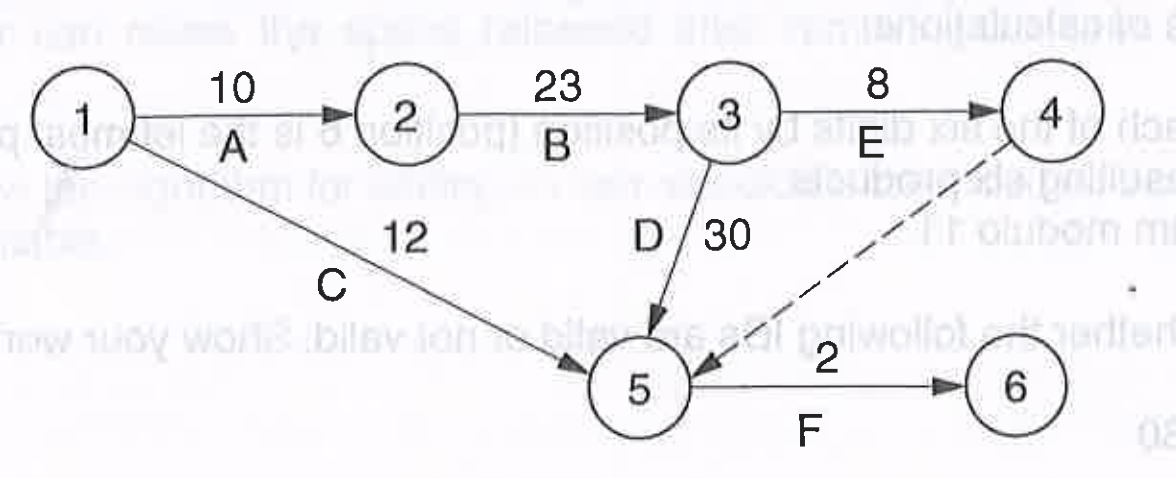
\includegraphics[width=0.5\paperwidth]{C:/Users/Admin/Desktop/Github/question_bank/LyX/static/img/9597-ALVL-2015-P2-Q1}
\par\end{center}
\begin{enumerate}
\item[(e)] {}
\begin{enumerate}
\item Describe \textbf{two} benefits that can be gained by producing a PERT
chart from the activity table. \hfill{}{[}2{]}
\item Explain the significance of the dashed line on the PERT chart. \hfill{}{[}2{]}
\item There are two errors on the PERT chart. identify these errors. Redraw
the PERT chart to show the changes needed to correct these errors.
\hfill{}{[}2{]}
\end{enumerate}
\item[(f)]  Using your PERT chart from part \textbf{(e)(iii)}: 
\begin{itemize}
\item State the minimum time in which the project could be completed.\hfill{}
{[}1{]}
\item By how many weeks can the start of the production of documentation
be delayed without delaying the whole project? \hfill{}{[}1{]}
\item Describe and give an example of concurrent activities.\hfill{} {[}2{]}
\item Describe and give an example of dependent activities. \hfill{}{[}2{]}
\end{itemize}
\end{enumerate}
Output from the system is made available to permitted staff via the
university intranet. However, the university intranet can be accessed
by all students and staff. both locally and remotely, via the lnternet.
The system needs security measures to prevent all types of unauthorised
access. 
\begin{enumerate}
\item[(g)]  Describe\textbf{ two} suitable physical security measures that could
be adopted. \hfill{}{[}4{]}
\item[(h)]  Describe \textbf{two} suitable software security measures that could
be adopted. \hfill{}{[}4{]}
\end{enumerate}
Following the success of the project, management decides that the
software system will be marketed to other universities. 
\begin{enumerate}
\item[(i)]  Explain how the university's investment in the software can be legally
protected. \hfill{}{[}2{]}
\end{enumerate}

 \newpage 

\item \textbf{{[}ALVL/9597/2015/P2/Q2{]} }

A stock control system requires that each stock item has a unique
ID consisting of six digits. The sixth digit is a check digit. This
check digit ensures that a value of 0 is the final result of the following
series of calculations:
\begin{itemize}
\item multiply each of the six digits by its position (position 6 is the
leftmost position)
\item sum the resulting six products
\item find the sum modulo 11.
\end{itemize}
\begin{enumerate}
\item Deduce whether the following IDs are valid or not valid. Show your
working. 
\begin{enumerate}
\item 810230 \hfill{}{[}2{]}
\item 371025 \hfill{}{[}2{]}
\end{enumerate}
\item The ID 483095 is a valid lD. Describe \textbf{one} typical data entry
error for this ID. Show how this error would be detected.\hfill{}
{[}3{]}
\item Describe a method of verification that can be used when an ID is entered
from a data entry form.\hfill{} {[}3{]}
\end{enumerate}

 \newpage 

\item \textbf{{[}ALVL/9597/2015/P2/Q3{]} }

A simple queue data structure is implemented using a one-dimensional
array and two pointers, Head and Tail, as shown:
\begin{center}
\begin{tabular}{r|l|l}
\multicolumn{1}{r}{} & \multicolumn{1}{l}{\texttt{Queue}} & \tabularnewline
\cline{2-2} 
\texttt{1} & \texttt{Mac} & \tabularnewline
\cline{2-2} 
\texttt{2} & \texttt{Ben} & $\impliedby$ \texttt{Head}\tabularnewline
\cline{2-2} 
\texttt{3} & \texttt{Dog} & \tabularnewline
\cline{2-2} 
\texttt{4} & \texttt{Can} & \tabularnewline
\cline{2-2} 
\texttt{5} & \texttt{Yog} & \tabularnewline
\cline{2-2} 
\texttt{6} & \texttt{Hur} & \tabularnewline
\cline{2-2} 
\texttt{7} &  & $\impliedby$ \texttt{Tail}\tabularnewline
\cline{2-2} 
\texttt{8} &  & \tabularnewline
\cline{2-2} 
\texttt{9} &  & \tabularnewline
\cline{2-2} 
\texttt{10} &  & \tabularnewline
\cline{2-2} 
\end{tabular}
\par\end{center}
\begin{enumerate}
\item Show the state of the above queue after: 
\begin{itemize}
\item two items, Dap and Eck, are added (in that order) 
\item one item is removed. \hfill{}{[}3{]}
\end{itemize}
When ten items have been added, this simple queue cannot accept any
further items. 
\item A first attempt at an algorithm for adding an item to this queue is:

\noindent\begin{minipage}[t]{1\columnwidth}%
\texttt{01 IF ..............................}

\texttt{02 \qquad{}THEN }

\texttt{03 \qquad{}\qquad{}OUTPUT \textquotedbl No more room to
add items\textquotedblright{} }

\texttt{04 \qquad{}ELSE }

\texttt{05 \qquad{}\qquad{}INPUT \textquotedbl New item to be added\textquotedbl ,
NewItem }

\texttt{06 \qquad{}\qquad{}Queue{[}..............................{]}
<- NewItem }

\texttt{O7 \qquad{}\qquad{}.............................. }

\texttt{O8 ENDIF }%
\end{minipage}

Write the pseudocode to show the completed lines 01, 06, and 07. \hfill{}{[}3{]}
\item Give the initial value for \texttt{Tail} when the queue is created
and justify your answer. \hfill{}{[}2{]}
\end{enumerate}
The programmer can reuse the space released after removing an item.
This maximises the available space.
\begin{enumerate}
\item[(d)]  Describe how the algorithm for adding an item should be amended
so that the released space is made available. \hfill{}{[}2{]}
\end{enumerate}

 \newpage 

\item \textbf{{[}ALVL/9597/2015/P2/Q4{]} }

An algorithm for converting a number n from denary to octal uses the
three built-in functions: 
\begin{center}
\begin{tabular}{|l|>{\raggedright}p{0.15\columnwidth}|>{\raggedright}p{0.25\columnwidth}|}
\hline 
\texttt{\hspace{0.01\columnwidth}}Function & \texttt{\hspace{0.01\columnwidth}}Description & \texttt{\hspace{0.01\columnwidth}}Example\tabularnewline
\hline 
\texttt{INTMOD(Number,Divisor)} & returns the remainder when the first parameter is divided by the second
parameter & \texttt{INTMOD(7,3) }returns 1\tabularnewline
\hline 
\texttt{INTDIV(Number,Divisor)} & returns the integer part when thefirst parameteris divided by the
second parameter. & \texttt{INTDIV(7,3) }returns 2\tabularnewline
\hline 
\texttt{SUBSTR(ThisString,Start,Length)} & forms a substring from ThisString, starting at Start (with first index
in string zero) and taking Length characters & \texttt{SUBSTR(``abcd'',1,2)} returns \texttt{``bc''}\tabularnewline
\hline 
\end{tabular}
\par\end{center}

Study the following pseudocode: 

\noindent %
\noindent\begin{minipage}[t]{1\columnwidth}%
\texttt{01 FUNCTION DenaryToOctal (n : INTEGER) RETURNS STRING }

\texttt{02 \qquad{}OctalDigits <- \textquotedbl 01234567\textquotedbl{} }

\texttt{03 \qquad{}IF n < 8 }

\texttt{04 \qquad{}\qquad{}THEN }

\texttt{05 \qquad{}\qquad{}\qquad{}TempString <- SUBSTR(OctalDigits,
n, 1) }

\texttt{06 \qquad{}\qquad{}ELSE }

\texttt{07 \qquad{}\qquad{}\qquad{}// '+' is the concatenation
operator }

\texttt{08 \qquad{}\qquad{}\qquad{}TempString <- DenaryToOctal(INTDIV(n,8))
+ SUBSTR(OctalDigits, INTMOD(n,8),1)) }

\texttt{09 \qquad{}ENDIF }

\texttt{10 \qquad{}RETURN TempString }

\texttt{11 ENDFUNCTION }%
\end{minipage}
\begin{enumerate}
\item Identify where and why this is a recursive function. \hfill{}{[}2{]}
\end{enumerate}
The diagram shows the execution of the call \texttt{DenaryToOctal(39)}. 
\begin{center}
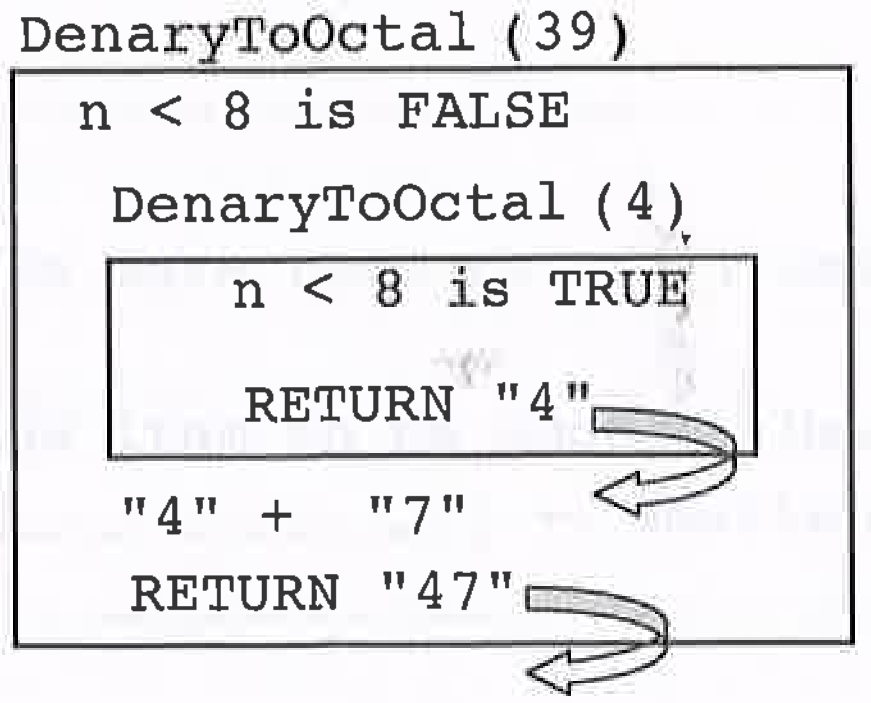
\includegraphics[width=0.5\paperwidth]{C:/Users/Admin/Desktop/Github/question_bank/LyX/static/img/9597-ALVL-2015-P2-Q4}
\par\end{center}
\begin{enumerate}
\item[(b)] Draw a similar diagram to show the execution of the call \texttt{DenaryToOctal(67)}.\hfill{}
{[}3{]}
\item[(c)] Changes are to be made to the function \texttt{DenaryToOctal()} so
that it converts denary numbers to hexadecimal.

Describe the changes: 
\begin{itemize}
\item that are essential to make the revised function work. 
\item that are non-essential but would help with the clarity of the pseudocode.\hfill{}
{[}5{]}
\end{itemize}
\end{enumerate}

 \newpage 

\item \textbf{{[}ALVL/9597/2015/P2/Q5{]} }

A program is to be written to test an insertion sort algorithm. A
top-down approach was used in the design of the program. The program,
\texttt{InsertionSortTester}, has a number of parts: 
\begin{itemize}
\item input integer values into the array 
\item output the initial values in the array 
\item output the sorted values in the array
\item perform the insertion sort 
\item validate the values 
\end{itemize}
\begin{enumerate}
\item Draw a diagram, which exhibits top-down design, for the \texttt{InsertionSortTester}
program. \hfill{}{[}3{]}

A list of data items is stored in the array \texttt{Values}. The pseudocode
for the insertion sort algorithm is: 

\noindent\begin{minipage}[t]{1\columnwidth}%
\texttt{01 FOR i <- 2 TO Arraysize }

\texttt{02 \qquad{}Temp <- Values{[}i{]} }

\texttt{03 \qquad{}j <- i\textemdash l }

\texttt{04 \qquad{}WHILE (j > 0) AND (Values {[}j{]} > Temp) }

\texttt{05 \qquad{}\qquad{}Values{[}j+1{]} <\textemdash{} Values
{[}j{]} }

\texttt{06 \qquad{}\qquad{}j <- j\textemdash l }

\texttt{07 \qquad{}\qquad{}ENDWHILE }

\texttt{08 \qquad{}\qquad{}Values {[}j+1{]} <- Temp }

\texttt{09 ENDFOR }%
\end{minipage}
\item The sort algorithm is to be tested using the sequence of numbers:
6, 8, 2 and 1. Copy and complete the trace table given below. 
\begin{center}
\begin{tabular}{|c|c|c|c||c|c|c|}
\hline 
\multicolumn{4}{|c||}{\texttt{Values}} &  &  & \tabularnewline
\hline 
\texttt{{[}1{]}} & \texttt{{[}2{]}} & \texttt{{[}3{]}} & \texttt{{[}4{]}} & \texttt{i} & \texttt{j} & \texttt{Temp}\tabularnewline
\hline 
\hline 
6 & 8 & 2 & 1 &  &  & \tabularnewline
\hline 
 &  &  &  &  &  & \tabularnewline
\hline 
 &  &  &  &  &  & \tabularnewline
\hline 
 &  &  &  &  &  & \tabularnewline
\hline 
 &  &  &  &  &  & \tabularnewline
\hline 
 &  &  &  &  &  & \tabularnewline
\hline 
 &  &  &  &  &  & \tabularnewline
\hline 
 &  &  &  &  &  & \tabularnewline
\hline 
 &  &  &  &  &  & \tabularnewline
\hline 
 &  &  &  &  &  & \tabularnewline
\end{tabular}
\par\end{center}

\hfill{}{[}6{]}
\item Explain why this particular algorithm is inefficient for an array
where the initial values are already in order.\hfill{} {[}2{]}
\item Give \textbf{two} different test cases for the program. Justify your
selection in each case.\hfill{} {[}4{]}
\end{enumerate}

 \newpage 

\item \textbf{{[}ALVL/9597/2015/P2/Q6{]} }

Students from several schools are entered for examinations in different
subjects. 

A relational database is to be used by the examination board to store
data about examination entries and results. Four tables present in
the database are STUDENT, SCHOOL, SUBJECT and STUDENT-SUBJECT.

Every time a student registers for a subject examination. a new row
is created in the STUDENT-SUBJECT table. When the result becomes available,
this is added to the appropriate row.

Each student, each school, and each subject has a unique identification
code.
\begin{enumerate}
\item {}
\begin{enumerate}
\item Draw an Entity-Relationship (E-R) diagram to show the relationship
between the STUDENT table and the SUBJECT table. \hfill{}{[}1{]}
\item State the type of relationship that exists between the STUDENT and
SUBJECT tables. \hfill{}{[}1{]}
\end{enumerate}
\item Draw an E-R diagram to show the relationship between the four tables
that provides for a fully normalised database design.\hfill{} {[}3{]}
\end{enumerate}
A table description can be expressed as: 

\texttt{TableName(Attribute1, Attribute2, Attribute3, ...)} 

The primary key is indicated by underlining one or more attributes. 

An incomplete STUDENT table is: 

\texttt{STUDENT(}\texttt{\uline{StudentID}}\texttt{, StudentName,
DateOfBirth) }
\begin{enumerate}
\item[(c)]  Give a table description for the SUBJECT table. Ensure there are
\textbf{two} attributes in addition to the primary key. \hfill{}{[}3{]}
\item[(d)]  Give a table description for the STUDENT-SUBJECT table. Ensure there
is \textbf{one} non-key attribute.\hfill{} {[}3{]}
\item[(e)] {} 
\begin{enumerate}
\item State the type of relationship that exists between the STUDENT and
the SCHOOL tables.\hfill{} {[}1{]}
\item Explain how the relationship between the STUDENT table and the SCHOOL
table is established. \hfill{}{[}3{]}
\end{enumerate}
\end{enumerate}

 \newpage 

\item \textbf{{[}ALVL/9597/2016/P1/Q1{]} }

High-level programming languages usually have libraries of commonly
used routines. These include random number generators. 

\subsubsection*{Task 1.1}

Write program code to generate 1000 random integers in the range 1
to 20. 

The program will:
\begin{itemize}
\item Maintain a count of how many times each number is produced 
\item Print out a frequency table. 

Example output:

\begin{tabular}{ll}
Integer & Frequency\tabularnewline
1: & 54\tabularnewline
2: & 48\tabularnewline
3: & 52\tabularnewline
4: & 43\tabularnewline
5: & 48\tabularnewline
6: & 51\tabularnewline
7: & 41\tabularnewline
8: & 48\tabularnewline
9: & 53\tabularnewline
10: & 51\tabularnewline
11: & 45\tabularnewline
12: & 54\tabularnewline
13: & 44\tabularnewline
14: & 40\tabularnewline
15: & 54\tabularnewline
16: & 59\tabularnewline
17: & 47\tabularnewline
18: & 49\tabularnewline
19: & 66\tabularnewline
20: & 53\tabularnewline
\end{tabular}
\end{itemize}

\subsubsection*{Evidence 1}

Your program code. 

Screenshot of the program output.\hfill{}{[}7{]}

Random numbers generated by computers are usually referred to as pseudo-random
numbers because they are generated by executing program code. 

One criterion of a good pseudo-random number generator is that every
number in the range has an equal chance of being generated. This means
if 200 numbers are generated in the range 1 to 10, the expected frequency
value of every number in this range is 20. 

The program code is to be amended to check how well the given pseudo-random
number generator meets this requirement.

\subsubsection*{Task 1.2}

Amend your program code to:
\begin{itemize}
\item Calculate the expected frequency
\item Output this expected frequency
\item Output the difference between the actual and the expected frequency
for each number in the range as a third column of the frequency table.
\end{itemize}

\subsubsection*{Evidence 2}

Your program code.

Screenshot of the program output.\hfill{}{[}5{]}

 \newpage 

\item \textbf{{[}ALVL/9597/2016/P1/Q2{]} }

Customers are identified by ID numbers. These ID numbers are to be
stored in a hash table. The hashing function to be used is 
\begin{center}
\texttt{Address <- IDnumber MOD Max }
\par\end{center}

The hash table is implemented as a one-dimensional array with elements
indexed 0 to \texttt{(Max-1)}. 

\subsubsection*{Task 2.1}

Write program code to: 
\begin{itemize}
\item Read ID numbers from a text file and store them in a hash table. For
the purpose of testing the program. Max is to be set to the value
20. 

Assume different IDs will hash to different addresses (no collisions). 
\item Print out the contents of the hash table in the order in which the
elements are stored in the array.
\end{itemize}
Use \texttt{KEYS.TXT} to test your program code.

\subsubsection*{Evidence 3}

Your program code. 

Screenshot of the program output.\hfill{} {[}7{]}

\subsubsection*{Task 2.2}

Amend your program code so that collisions can be managed using open
hashing. This means a collision is resolved by searching sequentially
from the hashed address for an empty location and storing the ID at
this empty location. 

Use \texttt{KEYS2.TXT} to test your program code. 

\subsubsection*{Evidence 4}

Your program code.

Screenshot of the program output. \hfill{}{[}4{]}

\subsubsection*{Task 2.3}

Add code to your Task 2.2 program. 

The program is to: 
\begin{itemize}
\item Take as input an ID number 
\item Search the hash table and output the address (index number) of the
hash table where the ID was found. 
\end{itemize}
Use \texttt{KEYS2.TXT} to test your program code. 

Run the program three times. Use the following inputs: 37, 77 and
97.

\subsubsection*{Evidence 5}

Your program code.

Screenshot of the program output. \hfill{}{[}7{]}

 \newpage 

\item \textbf{{[}ALVL/9597/2016/P1/Q3{]} }

A binary tree Abstract Data Type (ADT) has commands to create a new
tree, add unique data items to the tree and print the tree.

The sequence of commands: 

\noindent %
\noindent\begin{minipage}[t]{1\columnwidth}%
\texttt{CreateNewTree }

\texttt{AddToTree(\textquotedbl Dave\textquotedbl ) }

\texttt{AddToTree(\textquotedbl Fred\textquotedbl ) }

\texttt{AddToTree(\textquotedbl Ed\textquotedbl ) }

\texttt{AddToTree(\textquotedbl Greg\textquotedbl ) }

\texttt{AddToTree(\textquotedbl Bob\textquotedbl ) }

\texttt{AddToTree(\textquotedbl Cid\textquotedbl ) }

\texttt{AddToTree(\textquotedbl Ali\textquotedbl )}%
\end{minipage}

would create the following binary tree:
\begin{center}
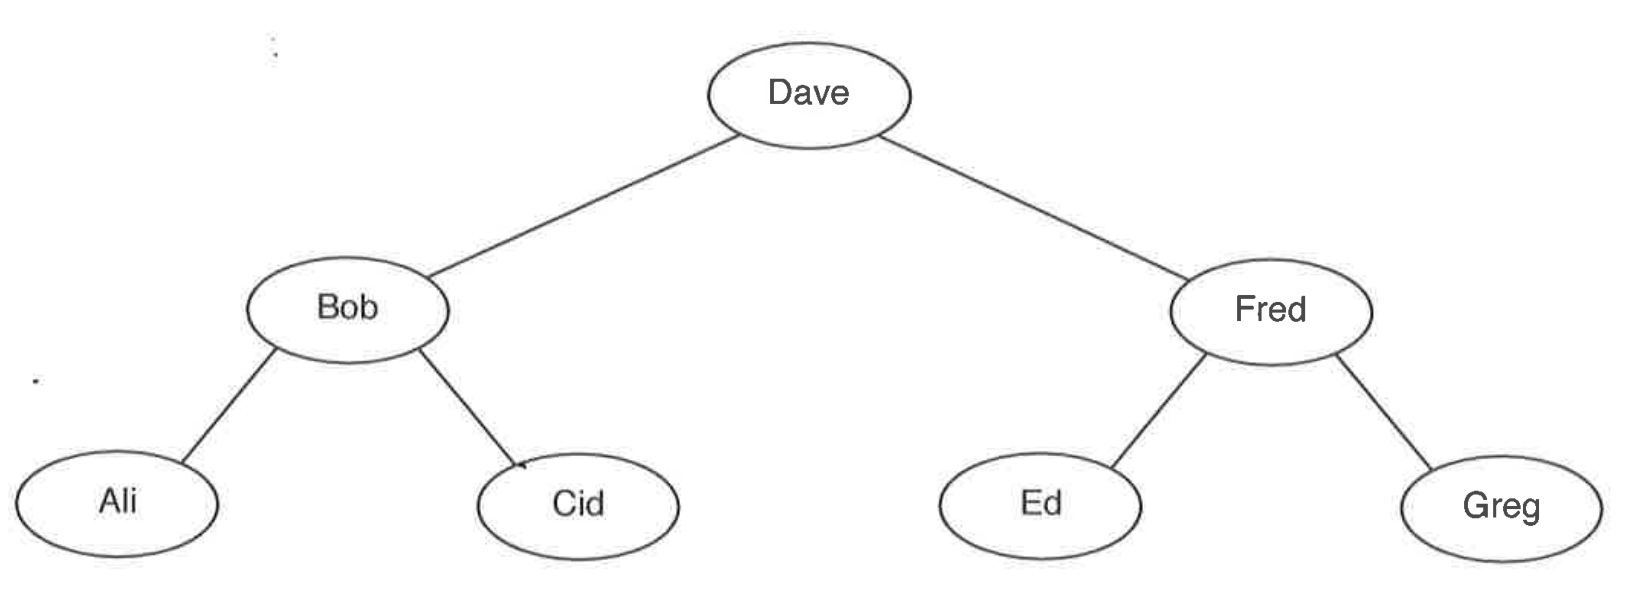
\includegraphics[width=0.5\paperwidth]{C:/Users/Admin/Desktop/Github/question_bank/static/img/9597-ALVL-2016-P1-Q3}
\par\end{center}

The program to implement this ADT will use the classes \texttt{Tree}
and \texttt{Node} designed as follows:
\begin{center}
\begin{tabular}{|l|}
\hline 
\texttt{\hspace{0.25\columnwidth}Tree}\tabularnewline
\hline 
\texttt{tree : ARRAY OF Node}\tabularnewline
\texttt{root : INTEGER}\tabularnewline
\tabularnewline
\hline 
\texttt{constructor()}\tabularnewline
\texttt{add(newItem)}\tabularnewline
\texttt{print() }\tabularnewline
\tabularnewline
\tabularnewline
\tabularnewline
\tabularnewline
\tabularnewline
\hline 
\end{tabular}%
\begin{tabular}{|l|}
\hline 
\hspace{0.25\columnwidth}\texttt{Node}\tabularnewline
\hline 
\texttt{data : STRING}\tabularnewline
\texttt{leftPtr : INTEGER}\tabularnewline
\texttt{rightPtr : INTEGER}\tabularnewline
\hline 
\texttt{constructor()}\tabularnewline
\texttt{setData(s : STRING)}\tabularnewline
\texttt{setLeftPtr(x : INTEGER)}\tabularnewline
\texttt{setRightPtr(y : INTEGER)}\tabularnewline
\texttt{getData() : STRING}\tabularnewline
\texttt{summary() : STRING}\tabularnewline
\texttt{getLeftPtr() : INTEGER}\tabularnewline
\texttt{getRightPtr() : INTEGER}\tabularnewline
\hline 
\end{tabular}
\par\end{center}

The program code must:
\begin{itemize}
\item Create a new tree, which has: 
\begin{itemize}
\item no nodes 
\item the root set to -1 
\end{itemize}
\item Use the root as a pointer to the first node in the tree 
\item Add a new node to the tree in the appropriate position 
\item Use the \texttt{print()} method to output, for each node, in array
order: 
\begin{itemize}
\item the data item 
\item the left pointer 
\item the right pointer. 
\end{itemize}
\end{itemize}

\subsubsection*{Task 3.1}

Write program code to define the classes \texttt{Tree} and \texttt{Node}. 

\subsubsection*{Evidence 6}

Your program code. \hfill{}{[}30{]}

\subsubsection*{Task 3.2}

The program is to be tested. 

Write a sequence of program statements to: 
\begin{itemize}
\item Create a tree 
\item Add the data items shown in the original list of ADT commands 
\item Print the array contents. 
\end{itemize}
Execute your program to test it. 

\subsubsection*{Evidence 7}

Your program code. 

Screenshot of test run.\hfill{} {[}3{]}

\subsubsection*{Task 3.3}

A method \texttt{inOrderTraversal()} is to be added, which outputs
the data stored in the tree in alphabetical order. 

Write program code to: 
\begin{itemize}
\item Implement this method 
\item Test the program code with the data from Task 3.2. 
\end{itemize}

\subsubsection*{Evidence 8}

Your program code. 

Screenshot of test run. \hfill{}{[}7{]}

 \newpage 

\item \textbf{{[}ALVL/9597/2016/P1/Q4{]} }

Numbers in Computing are often represented in hexadecimal form. 

A program is required to convert a hexadecimal number into a denary
number and vice versa. 

\subsubsection*{Task 4.1}

Write program code with the following specification: .
\begin{itemize}
\item Input a hexadecimal number as a string 
\item Validate the input 
\item Calculate the denary value of each hexadecimal digit (write this code
as a function)
\item Calculate the denary value of the hexadecimal number input
\item Output the denary value. 
\end{itemize}

\subsubsection*{Evidence 9}

Your program code. \hfill{}{[}10{]}

\subsubsection*{Task 4.2}

Draw up a list of \textbf{three} suitable test cases. Complete a table
with the following headings: 
\begin{center}
\begin{tabular}{|l|l|l|}
\hline 
Hexadecimal Number & Purpose of the test & Expected output\tabularnewline
\hline 
 &  & \tabularnewline
\hline 
 &  & \tabularnewline
\hline 
 &  & \tabularnewline
\hline 
\end{tabular}
\par\end{center}

Provide screenshot evidence for your testing. 

\subsubsection*{Evidence 10}

The completed table. 

Screenshots for each test data run. \hfill{}{[}5{]} 

\subsubsection*{Task 4.3}

Write additional code to convert a denary number into a hexadecimal
number. 

\subsubsection*{Evidence 11}

Your program code. \hfill{}{[}10{]}

\subsubsection*{Task 4.4}

Draw up a list of\textbf{ three} suitable test cases. Complete a table
with the following headings:
\begin{center}
\begin{tabular}{|l|l|l|}
\hline 
Denary Number & Purpose of the test & Expected output\tabularnewline
\hline 
 &  & \tabularnewline
\hline 
 &  & \tabularnewline
\hline 
 &  & \tabularnewline
\hline 
\end{tabular}
\par\end{center}

Provide screenshot evidence for your testing.

\subsubsection*{Evidence 12}

The completed table.

Screenshots for each test data run. \hfill{}{[}5{]}

 \newpage 

\item \textbf{{[}ALVL/9597/2016/P2/Q1{]} }

Many elderly people spend later life in a nursing home. The Ministry
of Health (MOH) requires each nursing home to keep detailed care records
for each resident. Care staff make daily entries in the care records
about all aspects of resident care. These care records are currently
paper-based documents. There is no common format for the documents
that different nursing homes use. 

Care staff do not have computer access to medical records that each
resident\textquoteleft s doctor holds. Nurses at a nursing home need
to keep their own medical records and to consult with residents\textquoteleft{}
doctors.

The MOH is planning an initiative to computerise all care records
and would like all nursing homes to use a common design for care records.

The MOH will send a project proposal which is to be circulated to
all nursing homes. This is to find out which homes would consider
taking part in a pilot project. The MOH's aim is to introduce a pilot
system into a single nursing home.

The MOH needs to find a software house to design and implement the
computerised care record system. It will send the project proposal
to software houses.

At a later date, all nursing homes will use the new computer system.
\begin{enumerate}
\item {} 
\begin{enumerate}
\item State \textbf{four} topics you would expect to find in this project
proposal.\hfill{} {[}4{]}
\item Describe the purpose of this project proposal. \hfill{}{[}2{]}
\end{enumerate}
Following production of the project proposal. the initial activities
with their expected times are as follows:
\begin{center}
\begin{tabular}{|c|>{\raggedright}p{0.5\columnwidth}|c|}
\hline 
\textbf{Label} & \texttt{\textbf{\hspace{0.01\columnwidth}}}\textbf{Activity } & \textbf{Time (weeks)}\tabularnewline
\hline 
A & Send the project proposal document to all nursing homes. & 5\tabularnewline
\hline 
B & Circulate the project proposal document to a number of software houses. & 6\tabularnewline
\hline 
C & Review the feedback. Note which nursing homes and software houses
have expressed interest.  & 2\tabularnewline
\hline 
D & identify doctors who look after residents in homes that have expressed
interest. Hold a presentation meeting to explain the proposed project
to these doctors. & 5\tabularnewline
\hline 
E & Presentation event for the chosen nursing home. & 2\tabularnewline
\hline 
\end{tabular}
\par\end{center}

\end{enumerate}
The Program Evaluation and Review Technique (PERT) chart for these
initial activities is shown below. 
\begin{center}
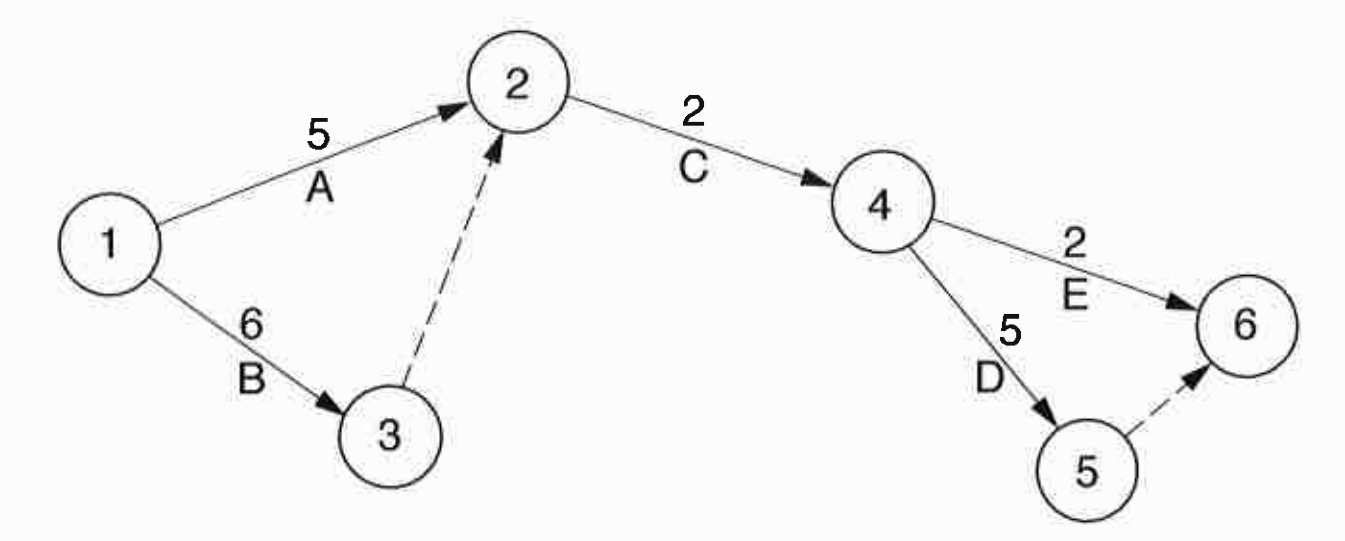
\includegraphics[width=0.5\paperwidth]{C:/Users/Admin/Desktop/Github/question_bank/static/img/9597-ALVL-2016-P2-Q1-1}
\par\end{center}
\begin{enumerate}
\item[(b)] {}
\begin{enumerate}
\item State the critical path for the initial activities. \hfill{}{[}1{]}
\item Calculate the minimum time these initial activities will take.\hfill{}
{[}1{]}
\end{enumerate}
\item[(c)] In activity E, the MOH presented more details about the project to
the manager and care staff of the chosen nursing home. The manager
and care staff raised a number of points about both social and ethical
issues associated with the project. 

Describe \textbf{three} points that could have been raised.\hfill{}
{[}6{]}
\end{enumerate}
Following activity E, the MOH decided the software house to which
it would award the contract. 

Following the initial project proposal. activities which make up the
system development cycle are shown below:
\begin{center}
\begin{tabular}{|c|>{\raggedright}p{0.5\columnwidth}|c|}
\hline 
\textbf{Label} & \texttt{\textbf{\hspace{0.01\columnwidth}}}\textbf{Activity} & \textbf{Time (weeks)}\tabularnewline
\hline 
F & Analysis & 12\tabularnewline
\hline 
G & Design & 15\tabularnewline
\hline 
H & Data entry of current care record data & 4\tabularnewline
\hline 
I & Initial testing & 10\tabularnewline
\hline 
J & Program development  & 14\tabularnewline
\hline 
K & Install new hardware in nursing home  & 3\tabularnewline
\hline 
L & Alpha testing & 2\tabularnewline
\hline 
M & Beta testing & 1\tabularnewline
\hline 
N & Implementation & 3\tabularnewline
\hline 
\end{tabular}
\par\end{center}

\begin{center}
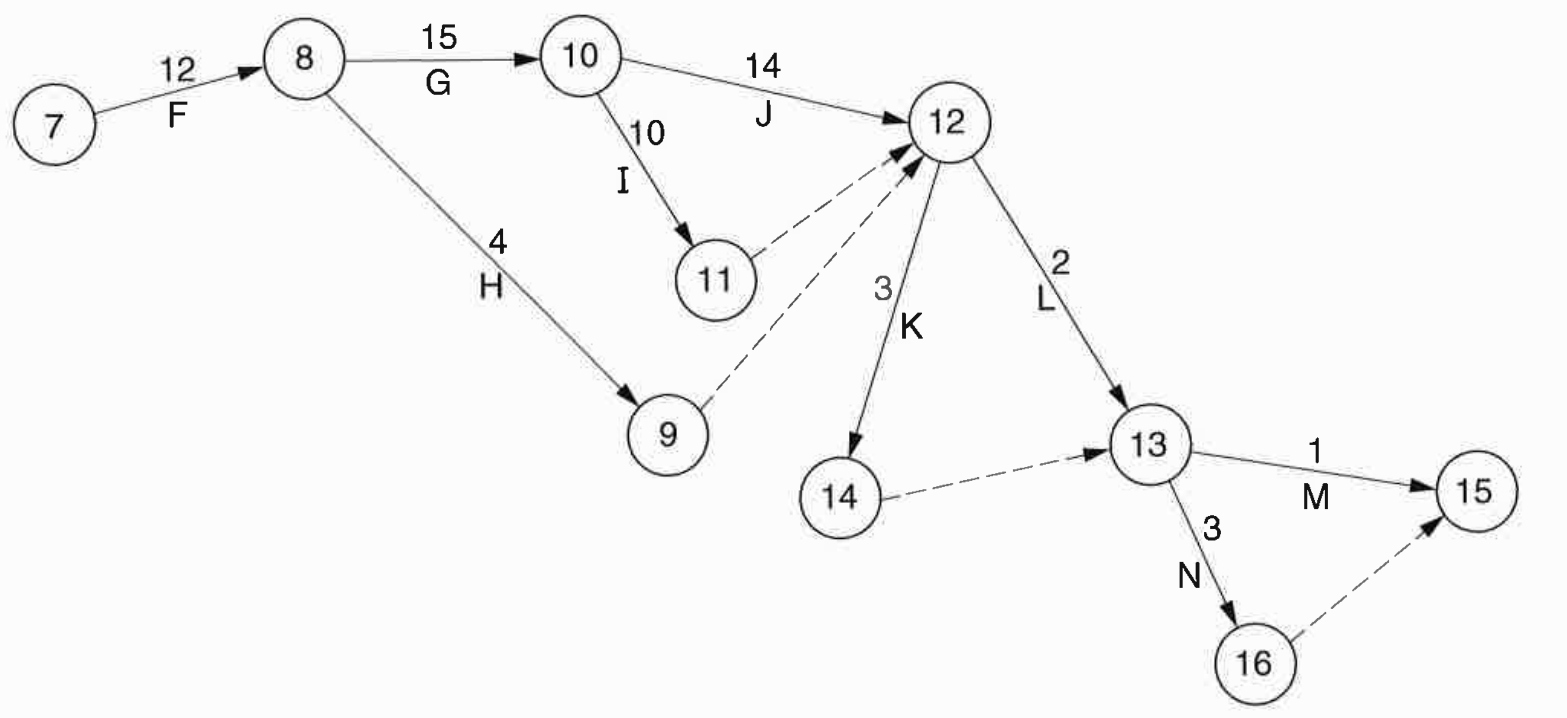
\includegraphics[width=0.5\paperwidth]{C:/Users/Admin/Desktop/Github/question_bank/static/img/9597-ALVL-2016-P2-Q1-2}
\par\end{center}
\begin{enumerate}
\item[(d)] The system development cycle starts at node (time point) 7.
\begin{enumerate}
\item The PERT chart shows four activities with dashed lines. Explain the
significance of the dashed lines.\hfill{} {[}1{]}
\item Explain the meanings of a dependent stage and concurrent stages in
a PERT chart. Give an example of each for this project. \hfill{}{[}4{]}
\item The table describes activity I as \textquoteleft initial testing'.
One category of initial testing is white-box testing.

Name and describe two other categories of initial testing. \hfill{}{[}4{]}
\item The PERT chart indicates that some testing can commence almost as
soon as program development does. Describe the type of program development
that would allow for this.\hfill{} {[}2{]}
\end{enumerate}
\item[(e)] An analyst from the software house carried out the analysis for the
project. 

Describe \textbf{three} examples of people whom the analyst consulted.
For each example. state: 
\begin{itemize}
\item the fact finding technique used 
\item the nature of the information that the analyst obtained. 
\end{itemize}
Each fact finding technique should be different.\hfill{} {[}6{]}
\item[(f)]  When the analysis stage was completed. the following decisions were
taken: 
\begin{itemize}
\item Each nursing home will store and manage its own care records data. 
\item Each nursing home will be provided with a local area network (LAN). 
\item The care record system on each LAN will use a client-server model
with a web interface for client computers. 
\end{itemize}
\begin{enumerate}
\item Explain the meaning of the term client-server model. \hfill{}{[}3{]}
\item State the \textbf{two} items of software that the LAN will use to
implement this client-server design. \hfill{}{[}2{]}
\end{enumerate}
\end{enumerate}
During the presentation event to doctors (part of activity D). the
doctors gave feedback. They said that they would like to have access
to the new computerised care records from their own offices. 
\begin{enumerate}
\item[(g)] A second phase of the project is to allow each nursing home access
to the medical data stored by doctors. This will involve connecting
the LAN for each nursing home to a number of doctors' surgery LANs. 
\begin{enumerate}
\item (l) State \textbf{two} methods for ensuring the security of access
to the care record network application. \hfill{}{[}2{]}
\item (ll) Give \textbf{two} methods for protecting the security of the
LAN. \hfill{}{[}2{]}
\end{enumerate}
\end{enumerate}

 \newpage 

\item \textbf{{[}ALVL/9597/2016/P2/Q2{]} }

A firm hires vehicles to customers. A customer usually makes a booking
a number of weeks before the start of the hire period. The customer
pays a deposit at the time of the booking and the balance when they
return the vehicle from hire.

At the time of the booking, the firm records the following data:
\begin{itemize}
\item customer data, including a customer reference code
\item booking date
\item hire start date
\item hire return date
\item type of vehicle
\item deposit taken
\end{itemize}
Vehicle types are coded as follows:
\begin{itemize}
\item Small car - SC
\item Large car - LC
\item Utility vehicle - UV
\end{itemize}
Each vehicle type has its own daily charge, for each day of the hire
period.

Each vehicle has a unique registration.

Customers may make more than one booking. The software will not allow
a customer to make more than one booking for the same start date.

The document below is an example of an invoice printed for the customer
when they return the vehicle and pay the balance due.
\begin{center}
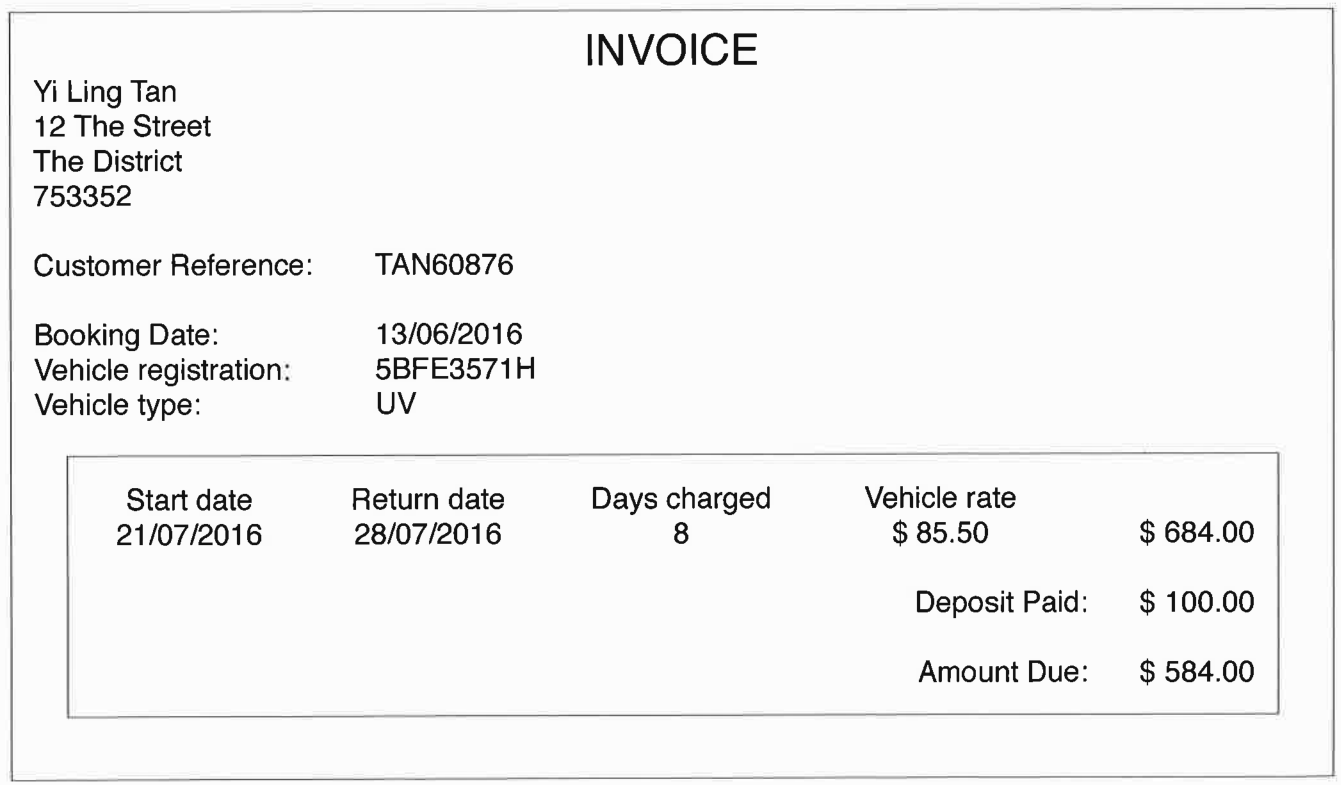
\includegraphics[width=0.5\paperwidth]{C:/Users/Admin/Desktop/Github/question_bank/static/img/9597-ALVL-2016-P2-Q2}
\par\end{center}
\begin{enumerate}
\item The firm wants to model this application using a relational database.
\begin{enumerate}
\item A database needs a number of tables to store the data for this application.
Draw the Entity-Relationship (E-R) diagram showing the tables and
the relationships between them. \hfill{}{[}6{]}
\item A table description can be expressed as: 

\texttt{TableName (}\texttt{\uline{Attributel}}\texttt{ , Attribute2
, Attribute3 , ....) }

The primary key is indicated by underlining one or more attributes. 

Write table descriptions for the tables you identified in \textbf{part
(i)}. \hfill{}{[}6{]}
\end{enumerate}
\item The firm implements the relational database using a Database Management
System (DBMS). It writes programs to access the data using a Graphical
User Interface (GUI). 

One program is for recording a new booking. 

The firm uses different types of components in a GUI for the display
and entry of data. 

Name \textbf{three} types of component that the booking form could
use and give the types of data it is used to capture. \hfill{} {[}3{]}
\end{enumerate}

 \newpage 

\item \textbf{{[}ALVL/9597/2016/P2/Q3{]} }

The recursive procedure \texttt{X} was two parameters, \texttt{Value}
and \texttt{Index}. The procedure processes the contents of an array,
\texttt{T}.

\noindent %
\noindent\begin{minipage}[t]{1\columnwidth}%
\texttt{01 PROCEDURE X(Value, Index)}

\texttt{02 \qquad{}IF T{[}Index{]} > 0}

\texttt{03 \qquad{}\qquad{}THEN}

\texttt{04 \qquad{}\qquad{}\qquad{}IF T{[}Index{]} > Value}

\texttt{05 \qquad{}\qquad{}\qquad{}\qquad{}THEN}

\texttt{06 \qquad{}\qquad{}\qquad{}\qquad{}\qquad{}X(Value, Index
{*} 2) }

\texttt{07 \qquad{}\qquad{}\qquad{}ENDIF}

\texttt{08 \qquad{}\qquad{}\qquad{}IF T{[}Index{]} < Value}

\texttt{09 \qquad{}\qquad{}\qquad{}\qquad{}THEN}

\texttt{10 \qquad{}\qquad{}\qquad{}\qquad{}\qquad{}X(Value, Index
{*} 2 + 1) }

\texttt{11 \qquad{}\qquad{}\qquad{}ENDIF}

\texttt{12 \qquad{}\qquad{}\qquad{}IF T{[}Index{]} = Value}

\texttt{13 \qquad{}\qquad{}\qquad{}\qquad{}THEN}

\texttt{14 \qquad{}\qquad{}\qquad{}\qquad{}\qquad{}OUTPUT \textquotedbl True\textquotedbl}

\texttt{15 \qquad{}\qquad{}\qquad{}ENDIF}

\texttt{l6 \qquad{}ENDIF}

\texttt{17 ENDPROCEDURE}%
\end{minipage}
\begin{enumerate}
\item {}
\begin{enumerate}
\item State what is meant by a recursive procedure. \hfill{}{[}1{]}
\item Give the two line numbers which indicate that procedure x is recursive.
\hfill{} {[}1{]}
\end{enumerate}
\item An array T is used to store the data for a binary tree. A program
places items in the array in the order in which they joined the tree
structure. 
\begin{center}
\begin{tabular}{|c|c|c|c|c|c|c|c|c|c|c|c|c|c|c|}
\hline 
1 & 2 & 3 & 4 & 5 & 6 & 7 & 8 & 9 & 10 & 11 & 12 & 13 & 14 & 15\tabularnewline
\hline 
17 & 11 & 19 & 9 & 12 & 18 & 23 & 0 & 4 & 0 & 0 & 0 & 0 & 0 & 0\tabularnewline
\hline 
\end{tabular}
\par\end{center}
\begin{enumerate}
\item Draw the binary tree for the array \texttt{T} dataset. \hfill{} {[}3{]}
\item Copy and then complete the trace table for the procedure call \texttt{X(18,
1)}.
\begin{center}
\begin{tabular}{|c|c|c|c|}
\hline 
Procedure call & \texttt{Value} & \texttt{Index} & Output\tabularnewline
\hline 
\texttt{1} & \texttt{18} & \texttt{1} & \tabularnewline
\hline 
 &  &  & \tabularnewline
\hline 
 &  &  & \tabularnewline
\hline 
 &  &  & \tabularnewline
\hline 
 &  &  & \tabularnewline
\hline 
\end{tabular} 
\par\end{center}

\begin{center}
\hfill{}{[}3{]}
\par\end{center}
\item Describe the purpose of procedure \texttt{X}. \hfill{}{[}2{]}
\end{enumerate}
\end{enumerate}

 \newpage 

\item \textbf{{[}ALVL/9597/2016/P2/Q4{]} }

Data is to be transmitted in packets between two computers. 

Each packet message can consist of: 
\begin{itemize}
\item upper case letters 
\item the <Space> character. 
\end{itemize}
Each packet has a start character (\#) and an end character (\#). 

A typical packet would be: 
\begin{center}
\texttt{\#ETA FROM SRE\#}
\par\end{center}
\begin{enumerate}
\item Describe\textbf{ two} checks that the receiving computer should make
for the integrity of:
\begin{itemize}
\item the individual bytes which make up a packet
\item the collection of bytes which makes up the packet. \hfill{} {[}4{]}
\end{itemize}
\item Describe \textbf{three} validation checks that the receiving computer
should pertorm on the packet. \hfill{}{[}6{]}
\end{enumerate}

 \newpage 

\item \textbf{{[}ALVL/9597/2016/P2/Q5{]} }

A programmer implements a linked list of surnames with a start pointer,
\texttt{StartPtr} and two one-dimensional arrays: 
\begin{itemize}
\item Array \texttt{Data} stores the surnames. 
\item Array \texttt{Ptr} stores the link pointers.
\item Both arrays have lower bound 1 and upper bound 3000. 
\end{itemize}
The purpose of procedure \texttt{InsertListItem} is to insert a new
surname to the linked list. 

Assume a function \texttt{NextFree()} is available and returns: 
\begin{itemize}
\item the index position for the array \texttt{Data} at which the new surname
is to be inserted 
\item -1 when the \texttt{Data} array is full. 
\end{itemize}
The programmer designs the algorithm as follows:

\noindent %
\noindent\begin{minipage}[t]{1\columnwidth}%
\texttt{01 PROCEDURE InsertListItem(NewSurname : STRING) }

\texttt{02 \qquad{}IF NextFree() = \textemdash 1 }

\texttt{03 \qquad{}\qquad{}THEN }

\texttt{04 \qquad{}\qquad{}\qquad{}OUTPUT \textquotedbl List is
full\textquotedbl{} }

\texttt{05 \qquad{}\qquad{}ELSE }

\texttt{O6 \qquad{}\qquad{}\qquad{}// input the surname }

\texttt{07 \qquad{}\qquad{}\qquad{}IF StartPtr = 0 }

\texttt{08 \qquad{}\qquad{}\qquad{}\qquad{}THEN }

\texttt{09 \qquad{}\qquad{}\qquad{}\qquad{}\qquad{}StartPtr w
NextFree() }

\texttt{10 \qquad{}\qquad{}\qquad{}\qquad{}\qquad{}Data{[}StartPtr{]}
e NewSurname }

\texttt{11 \qquad{}\qquad{}\qquad{}\qquad{}ELSE }

\texttt{12 \qquad{}\qquad{}\qquad{}\qquad{}\qquad{}// traverse
the linked list to find the position }

\texttt{13 \qquad{}\qquad{}\qquad{}\qquad{}\qquad{}// at which
to insert NewSurname}

$\vdots$

\texttt{\qquad{}\qquad{}\qquad{}\qquad{}ENDIF }

\texttt{\qquad{}\qquad{}ENDIF }

\texttt{\qquad{}ENDPROCEDURE}%
\end{minipage}
\begin{enumerate}
\item Describe the state of the linked list. if the condition \texttt{StartPtr
= 0} in line \texttt{07} is \texttt{True}. {[}1{]} 
\item It is now necessary to complete the design for procedure \texttt{InsertListItem}. 
\begin{enumerate}
\item The pseudocode already uses some variables. 

Copy the table below and complete it to show any extra variables that
you will need to use. 
\begin{center}
\begin{tabular}{|c|c|c|}
\hline 
\textbf{Variable} & \textbf{Data Type} & \textbf{Description}\tabularnewline
\hline 
 &  & \tabularnewline
\hline 
 &  & \tabularnewline
\hline 
 &  & \tabularnewline
\hline 
 &  & \tabularnewline
\hline 
 &  & \tabularnewline
\hline 
\end{tabular}
\par\end{center}

\hfill{}{[}3{]}
\item Write the pseudocode for line \texttt{14} onwards to complete the
procedure. \hfill{}{[}6{]}
\end{enumerate}
\end{enumerate}

 \newpage 

\item \textbf{{[}ALVL/9597/2016/P2/Q6{]} }

A real-estate management company owns a number of residential and
business units. When the company first acquires a unit, it often requires
renovation work. The company records the renovation cost.

A residential unit will be a house or an individual flat within a
building. A business unit will be either an office building, a storage
unit or a factory.

A residential unit is either advertised for sale, with the company
looking to make a profit, or retained for rental. If the unit is sold,
the sale price is recorded. If the unit is retained, the monthly rental
charged, the start date and length of the rental (in months) are recorded.

A business unit has a long term lease, which is usually 10 years or
longer. The company records the nature of the business. it does not
offer any of its business units for sale. 

Other data recorded for a unit include: purchase price, purchase date,
number of rooms, floor space, whether or not a lift is present. The
company records whether the house has a garage and whether it has
a garden. 

A programmer will develop an application, using object-oriented programming
to store and process the company\textquoteright s data. 
\begin{enumerate}
\item Draw a class diagram, with base class \texttt{UNIT}, showing: 
\begin{itemize}
\item appropriate sub-class(es)
\item inheritance 
\item the properties required 
\item appropriate methods, including \textbf{one} pair of \textquoteleft get\textquoteright{}
and \textquoteleft set\textquoteleft{} methods for \textbf{one} of
the properties.\hfill{} {[}8{]}
\end{itemize}
\item The company has recently purchased a number of units that they want
to renovate as a \textquoteleft block of flats\textquoteright{} (a
number of self-contained flats in the same building). Once the renovation
is complete, the company may offer a block of flats for sale. Alternatively,
it may retain the unit and advertise each individual flat for rental. 

Explain how this would affect the design in \textbf{part (a)}. \hfill{}{[}3{]}
\item {}
\begin{enumerate}
\item Explain the meaning of the term encapsulation. \hfill{}{[}2{]}
\item Explain the meaning of the term polymorphism. \hfill{}{[}2{]}
\end{enumerate}
\end{enumerate}

 \newpage 

\item \textbf{{[}ALVL/9597/2017/P1/Q1{]} }

A role-playing computer game includes a list of items called the inventory.
This inventory can be represented using a one-dimensional (1 -D) array
or a list structure. 

\texttt{INVENTORY.TXT} is a text file containing the items from the
computer game inventory. Each item type can have many occurrences.
For example: 

\begin{tabular}{lll}
\textbf{Inventory} &  & \textbf{ItemType}\tabularnewline
Iron Ore &  & Iron Ore\tabularnewline
Stone &  & Stone\tabularnewline
Sticky Piston &  & Sticky Piston\tabularnewline
Glass &  & Glass \tabularnewline
Stone &  & Sand \tabularnewline
Stone &  & \tabularnewline
Sand &  & \tabularnewline
Sticky Piston &  & \tabularnewline
Iron Ore &  & \tabularnewline
\end{tabular}

\subsubsection*{Task 1.1}

Design and write program code to: 
\begin{itemize}
\item read the entire contents of \texttt{INVENTORY.TXT} to an appropriate
data structure called Inventory 
\item find each item type in this inventory and write these into a second
similar data structure called \texttt{ItemTypes} 
\item count the number of each item type in the inventory and store this
in a third similar data structure called \texttt{ItemCounts }
\item display the contents of the ItemTypes and ItemCounts data structures
using the format given below. 
\end{itemize}
Example run of the program: 

\begin{tabular}{lllll}
\textbf{Inventory} &  & \multicolumn{3}{l}{The output generated from this input would be:}\tabularnewline
Iron Ore &  &  &  & \tabularnewline
Stone &  & \textbf{ItemType} &  & \textbf{Count}\tabularnewline
Sticky Piston &  &  &  & \tabularnewline
Glass &  & Iron Ore &  & 2\tabularnewline
Stone &  & Stone &  & 3\tabularnewline
Stone &  & Sticky Piston &  & 2\tabularnewline
Sand &  & Glass &  & 1\tabularnewline
Sticky Piston &  & Sand &  & 1\tabularnewline
Iron Ore &  &  &  & \tabularnewline
\end{tabular}

\subsubsection*{Evidence 1}

Your program code.\hfill{}{[}14{]}

\subsubsection*{Evidence 2}

Screenshot of your output. \hfill{}{[}1{]}

 \newpage 

\item \textbf{{[}ALVL/9597/2017/P1/Q2{]} }

Every published book has an international Standard Book Number (ISBN).
This ISBN is a 9-digit number plus a check digit which is calculated
and added to the end of the number. A weighted-modulus method is used
to calculate the check digit. 

This method uses a weighted modulus 11. If the check digit is calculated
as 10. it is replaced with the character 'X'. Where the check digit
is calculated as 11, it will be replaced with 0. 

\noindent %
\begin{tabular}{l}
184146208 will be calculated as\tabularnewline
$1\times10=10$\tabularnewline
$8\times9=72$\tabularnewline
$4\times8=32$\tabularnewline
$1\times7=7$\tabularnewline
$4\times6=24$\tabularnewline
$6\times5=30$\tabularnewline
$2\times4=8$\tabularnewline
$0\times3=0$\tabularnewline
$8\times2=16$\tabularnewline
Total = 199\tabularnewline
$199/11=18$ remainder 1\tabularnewline
$11-1=10$\tabularnewline
Therefore, 10 is replaced with X:\tabularnewline
ISBN is 184146208\textbf{X}\tabularnewline
\end{tabular}%
\begin{tabular}{l}
034085045 will be calculated as\tabularnewline
$0\times10=0$\tabularnewline
$7\times9=63$\tabularnewline
$5\times8=40$\tabularnewline
$1\times7=7$\tabularnewline
$5\times6=30$\tabularnewline
$4\times5=20$\tabularnewline
$9\times4=36$\tabularnewline
$2\times3=6$\tabularnewline
$6\times2=12$\tabularnewline
Total = 154\tabularnewline
$154/11=14$ remainder 0\tabularnewline
$11-0=11$\tabularnewline
Therefore, 11 is replaced with 0:\tabularnewline
ISBN is 034085045\textbf{0}\tabularnewline
\end{tabular}%
\begin{tabular}{l}
075154926 will be calculated as\tabularnewline
$0\times10=0$\tabularnewline
$3\times9=27$\tabularnewline
$4\times8=32$\tabularnewline
$0\times7=0$\tabularnewline
$8\times6=48$\tabularnewline
$5\times5=25$\tabularnewline
$0\times4=0$\tabularnewline
$4\times3=12$\tabularnewline
$5\times2=10$\tabularnewline
Total = 214\tabularnewline
$214/11=19$ remainder 5\tabularnewline
$11-5=6$\tabularnewline
Therefore, 6 is added to the\tabularnewline
end of the ISBN: 075154926\textbf{6} \tabularnewline
\end{tabular}

\subsubsection*{Task 2.1}

Study the identifier table and the incomplete recursive algorithm
on the opposite page. 

The missing lines in the algorithm are labelled \textbf{A}, \textbf{B}
and \textbf{C}. 

Write the\textbf{ three} missing lines of code. Label each as \textbf{A},
\textbf{B} or \textbf{C}. \hfill{} {[}3{]}

\subsubsection*{Evidence 3}

The three missing lines of code. \hfill{}{[}3{]}
\begin{center}
\begin{tabular}{|l|c|l|}
\hline 
\textbf{Identifier} & \textbf{Data Type} & \textbf{Description}\tabularnewline
\hline 
\texttt{Number} & \texttt{STRING} & The ISBN to be processed\tabularnewline
\hline 
\texttt{Digit} & \texttt{lNTEGER} & A digit from the iSBN to be processed\tabularnewline
\hline 
\texttt{Total} & \texttt{INTEGER} & Running total for modulus calculation\tabularnewline
\hline 
\texttt{NewNumber} & \texttt{STRING} & A version of the list string shortened by removing the first character\tabularnewline
\hline 
\texttt{CheckDigit} & \texttt{STRING} & The calculated check digit value\tabularnewline
\hline 
\texttt{CalcModulus} & \texttt{INTEGER} & Used to store the result of \texttt{(Total MOD 11)}\tabularnewline
\hline 
\texttt{CheckValue} & \texttt{INTEGER} & Used to store the result of \texttt{(11 - CalcModulus)}\tabularnewline
\hline 
\end{tabular}
\par\end{center}

\noindent %
\noindent\begin{minipage}[t]{1\columnwidth}%
\texttt{FUNCTION CalCheckDigit(Number AS STRING, Total AS INTEGER)
RETURNS STRING }

\texttt{\qquad{}IF LENGTH(Number) > 1 THEN }

\texttt{\qquad{}\qquad{}Digit <- INTEGER(LEFT(Number,1)) }

\texttt{\qquad{}\qquad{}Total <- Total + (Digit {*} (LENGTH(Number)+1)) }

\texttt{\qquad{}\qquad{}NewNumber <- RIGHT(Number, LENGTH(Number)-1) }

\texttt{\qquad{}\qquad{}CheckDigit <- .................. A ................. }

\texttt{\qquad{}ELSE }

\texttt{\qquad{}\qquad{}Digit <- INTEGER(LEFT(Number,1)) }

\texttt{\qquad{}\qquad{}Total <- Total + (Digit 1 (LENGTH(Number)+1)) }

\texttt{\qquad{}\qquad{}CalcModulus <- Total MOD 11 }

\texttt{\qquad{}\qquad{}CheckValue <- 11 - CalcModulus }

\texttt{\qquad{}\qquad{}IF CheckValue = 11 THEN }

\texttt{\qquad{}\qquad{}\qquad{}RETURN STRING(O) }

\texttt{\qquad{}\qquad{}ELSE }

\texttt{\qquad{}\qquad{}\qquad{}IF CheckValue = 10 THEN }

\texttt{\qquad{}\qquad{}\qquad{}....................... B .......................... }

\texttt{\qquad{}\qquad{}\qquad{}ELSE }

\texttt{\qquad{}\qquad{}\qquad{}RETURN STRING(CheckValue) }

\texttt{\qquad{}\qquad{}\qquad{}ENDIF }

\texttt{\qquad{}\qquad{}ENDIF }

\texttt{\qquad{}ENDIF }

\texttt{\qquad{}IF LENGTH(Number) = 9 THEN }

\texttt{\qquad{}\qquad{}RETURN .................... C .................... }

\texttt{\qquad{}ELSE }

\texttt{\qquad{}\qquad{}RETURN CheckDigit; }

\texttt{\qquad{}ENDIF }

\texttt{END FUNCTION}

\bigskip{}

\texttt{// Calculate ISBN, an example of how the function is called. }

\texttt{// Second parameter is always 0. }

\texttt{ISBN = CalCheckDigit(\textquotedbl 184146208\textquotedbl ,0)}%
\end{minipage}

\subsubsection*{Task 2.2}

Write a program to implement the ISBN program using the \texttt{CalCheckDigit}
function.

The program will:
\begin{itemize}
\item read the entire contents of the file \texttt{ISBNPRE.TXT} (seven 9-digit
lSBNs without check digits) into an appropriate data structure
\item use the function \texttt{CalCheckDigit} to calculate the result (ISBN
with check digit) for each entry in the file
\item write each result (ISBN with check digit) to the screen.
\end{itemize}

\subsubsection*{Evidence 4}

Your program code for Task 2.2. \hfill{}{[}11{]}

\subsubsection*{Evidence 5}

Screenshot of the results of processing the \texttt{ISBNPRE.TXT} file.\hfill{}{[}1{]}

 \newpage 

\item \textbf{{[}ALVL/9597/2017/P1/Q3{]} }

A data structure is required to store 25 nodes. A linked list is maintained
of all the nodes. A node contains a data value and two pointers: a
left pointer and a right pointer. 

Items in the list are initially linked using their \texttt{LeftChild}
pointers. 

Each node ls implemented as an instance of the class \texttt{ConnectionNode}.
The class ConnectionNode has the following properties: 
\begin{center}
\begin{tabular}{|l|l|l|}
\hline 
\multicolumn{3}{|c|}{\texttt{Class: Connection Node}}\tabularnewline
\hline 
\multicolumn{3}{|c|}{Attributes}\tabularnewline
\hline 
\texttt{\hspace{0.01\columnwidth}}Identifier & \texttt{\hspace{0.01\columnwidth}}Data Type & \texttt{\hspace{0.05\columnwidth}}Description\tabularnewline
\hline 
\texttt{DataValue} & \texttt{STRING} & The node data\tabularnewline
\hline 
\texttt{LeftChild} & \texttt{INTEGER} & The left node pointer \tabularnewline
\hline 
\texttt{RightChild} & \texttt{INTEGER} & The right node pointer\tabularnewline
\hline 
\end{tabular}
\par\end{center}

The structure for the linked list is implemented as follows: 
\begin{center}
\begin{tabular}{|l|c|l|}
\hline 
\texttt{\hspace{0.01\columnwidth}}Identifier & Data Type & \texttt{\hspace{0.05\columnwidth}}Description\tabularnewline
\hline 
\texttt{RobotData} & \texttt{ARRAY {[}l : 25{]} OF ConnectionNode} & An array used to store the\tabularnewline
 &  & 25 nodes.\tabularnewline
\hline 
\texttt{Root} & \texttt{INTEGER} & Index for the root position \tabularnewline
 &  & of the \texttt{RobotData} array\tabularnewline
\hline 
\texttt{NextFreeChild} & \texttt{INTEGER} & Index for the next \tabularnewline
 &  & available empty node\tabularnewline
\hline 
\end{tabular}
\par\end{center}

The first available node Is indicated by \texttt{NextFreeChild}. The
initial value of \texttt{Root} is 1 and the initial value of \texttt{NextFreeChild}
is 1.

The diagram shows the empty data structure with the linked list to
record the unused nodes. 
\begin{center}
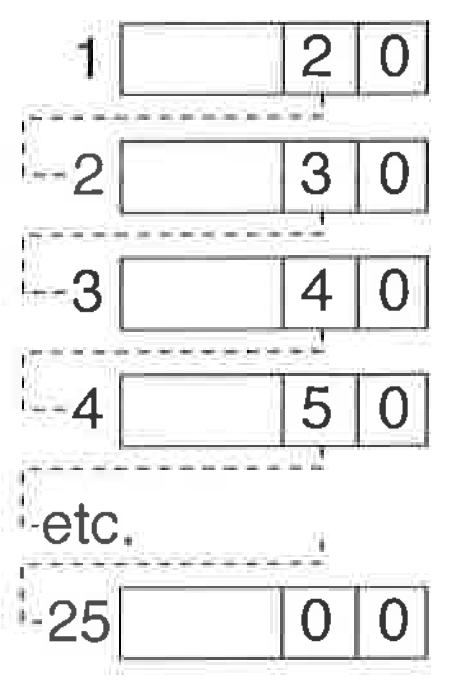
\includegraphics[width=0.125\paperwidth]{C:/Users/Admin/Desktop/Github/question_bank/LyX/static/img/9597-ALVL-2017-P1-Q3-1}
\par\end{center}

\subsubsection*{Task 3.1}

Write the program code to declare the \textbf{empty} data structure
and linked list of 25 unused nodes. Add statement(s) to initiallse
the empty data structure.

\subsubsection*{Evidence 6}

Your program code for Task 3.1. \hfill{}{[}12{]}

This data structure is used to record the possible routes for a robot
to travel from a node A to a node Z. The following data structure
illustrates many possible routes, for example, A$\rightarrow$D$\rightarrow$K$\rightarrow$L$\rightarrow$M$\rightarrow$Z.
It is only possible to move to one of two possible nodes; for example,
from node A, the only move is to node B or node D.
\begin{center}
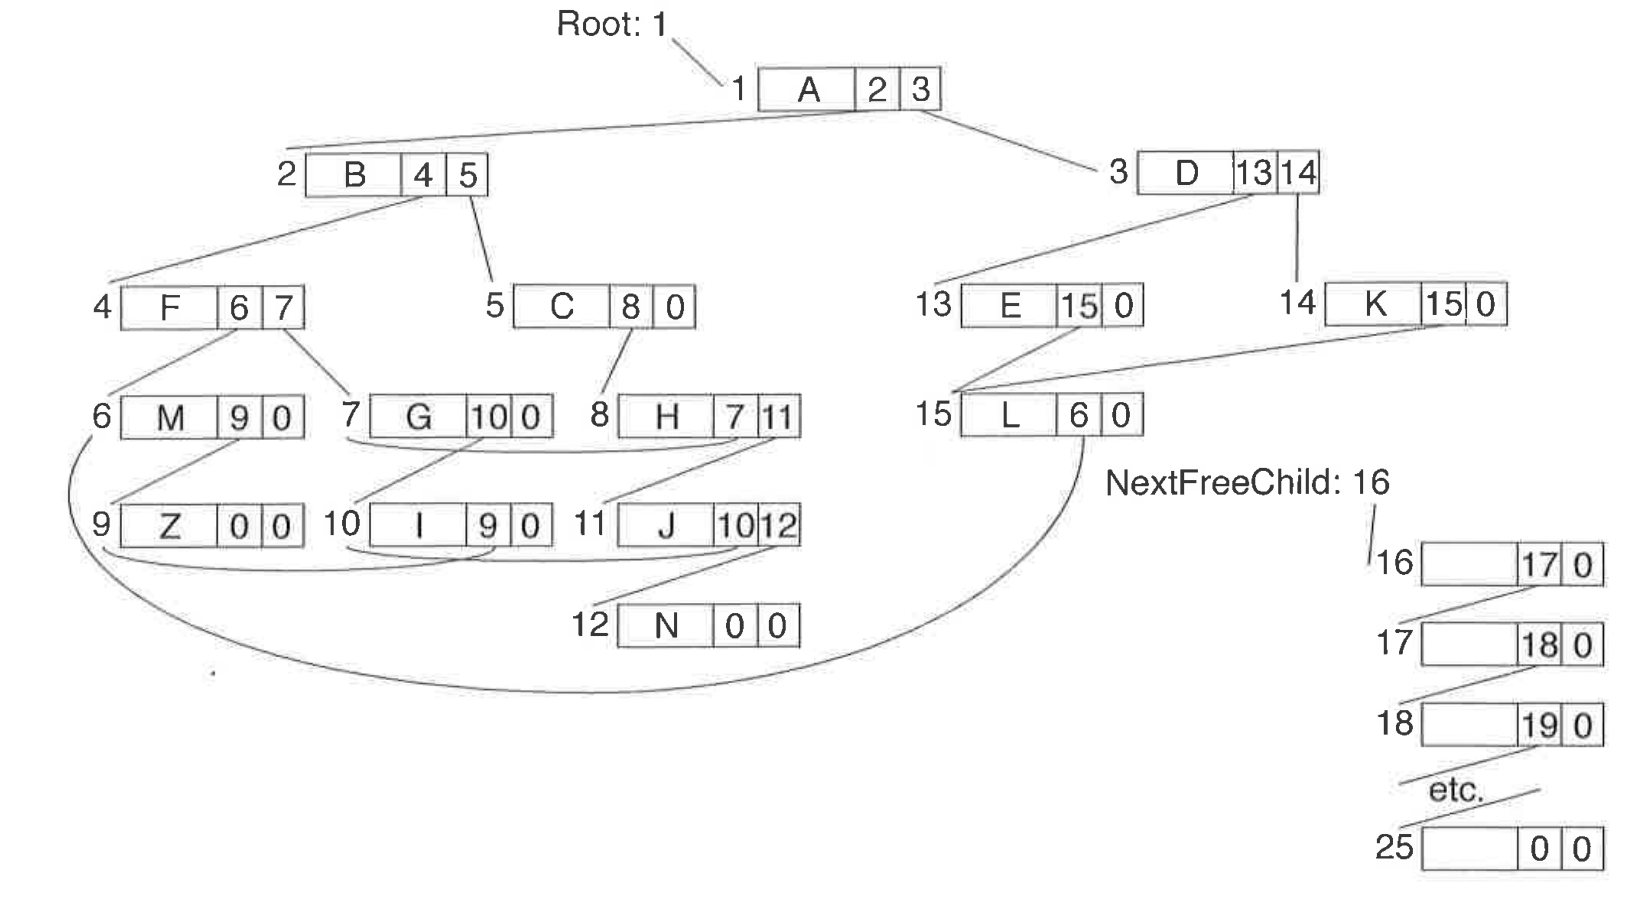
\includegraphics[width=0.5\paperwidth]{C:/Users/Admin/Desktop/Github/question_bank/LyX/static/img/9597-ALVL-2017-P1-Q3-2}
\par\end{center}

This data structure has 15 nodes (A to N and Z) but for future development
a maximum of 25 nodes is specified. All nodes are unique.

The pseudocode on the next page can be used to add a node to the data
structure. The procedure \texttt{AddToRobotData} uses the parameters
\texttt{NewDataItem}, \texttt{ParentItem} and \texttt{ThisMove}.

The parameter \texttt{ThisMove} holds the move made to create this
new item (\textquoteleft L' for LeftChild, \textquoteleft R' for RightChild,
\textquoteleft X\textquoteright{} for initial state/root), and the
\texttt{ParentItem} parameter holds the value of the parent item which
points to this \texttt{NewDataItem}.
\begin{center}
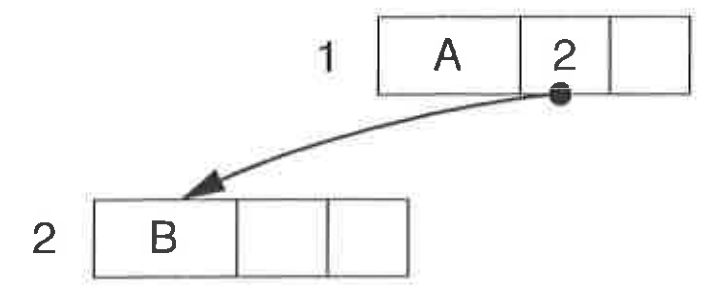
\includegraphics[width=0.25\paperwidth]{C:/Users/Admin/Desktop/Github/question_bank/LyX/static/img/9597-ALVL-2017-P1-Q3-3}
\par\end{center}

To add node B as shown, the procedure call would be \texttt{AddToRobotData
('B', \textquoteleft A', 'L')} . The parameters used would be: 

\texttt{B}, the new node 

\texttt{A}, the parent node 

\texttt{L}, the location of the child (which has an index of 2) is
recorded in \texttt{LeftChild} of A.

The following pseudocode (available in PS EUDOCODE\_TASK\_3\_2 . TXT)
can be used to add a node to the data structure.

\noindent %
\noindent\begin{minipage}[t]{1\columnwidth}%
\texttt{FUNCTION FindNode(NodeValue) RETURNS INTEGER }

\texttt{\qquad{}Found <- FALSE}

\texttt{\qquad{}CurrentPosition <- Root }

\texttt{\qquad{}REPEAT }

\texttt{\qquad{}\qquad{}IF RobotData{[}CurrentPosition{]}.DataValue
= NodeValue THEN }

\texttt{\qquad{}\qquad{}\qquad{}Found <- TRUE }

\texttt{\qquad{}\qquad{}ELSE }

\texttt{\qquad{}\qquad{}\qquad{}CurrentPosition <- CurrentPosition
+ 1 }

\texttt{\qquad{}\qquad{}ENDIF }

\texttt{\qquad{}UNTIL Found = TRUE OR CurrentPosition > 25 }

\texttt{\qquad{}IF CurrentPOSition > 25 THEN }

\texttt{\qquad{}\qquad{}RETURN 0}

\texttt{\qquad{}ELSE }

\texttt{\qquad{}\qquad{}RETURN CurrentPosition }

\texttt{\qquad{}ENDIF }

\texttt{ENDFUNCTION}

\bigskip{}

\texttt{PROCEDURE AddToRobotData(NewDataItem, ParentItem, ThisMove) }

\texttt{\qquad{}\qquad{}IF Root = 1 AND NextFreeChild = 1 THEN }

\texttt{\qquad{}\qquad{}\qquad{}NextFreeChild <- RobocData{[}NextFreeChild{]}.LeftChild }

\texttt{\qquad{}\qquad{}\qquad{}RobotDataIRoot{]}.LeftChild <-
0 }

\texttt{\qquad{}\qquad{}\qquad{}RobotData{[}Root{]}.DataValue <-
NewDataItem }

\texttt{\qquad{}\qquad{}ELSE }

\texttt{\qquad{}\qquad{}\qquad{}// does the parent exist? . }

\texttt{\qquad{}\qquad{}\qquad{}ParentPosition <- FindNode(ParentItem) }

\texttt{\qquad{}\qquad{}\qquad{}IF RarentPosition > 0 THEN // parent
exists }

\texttt{\qquad{}\qquad{}\qquad{}\qquad{}// does the child exist? }

\texttt{\qquad{}\qquad{}\qquad{}\qquad{}ExistingChild <- FindNode(NewDataItem)
' }

\texttt{\qquad{}\qquad{}\qquad{}\qquad{}IF ExistingChild > 0 THEN
// child exists }

\texttt{\qquad{}\qquad{}\qquad{}\qquad{}\qquad{}ChildPointer
<- ExistingChild }

\texttt{\qquad{}\qquad{}\qquad{}\qquad{}ELSE }

\texttt{\qquad{}\qquad{}\qquad{}\qquad{}ChildPointer <- NextFreeChild }

\texttt{\qquad{}\qquad{}\qquad{}\qquad{}NextFreeChild <- RobotDataINextFreeChild\}.LeftChild }

\texttt{\qquad{}\qquad{}\qquad{}\qquad{}RobotData{[}ChildPointer{]}.LeftChild
<- 0 }

\texttt{\qquad{}\qquad{}\qquad{}\qquad{}RobotData{[}ChildPointer{]}.DataValue
<- NewDataItem }

\texttt{\qquad{}\qquad{}\qquad{}\qquad{}ENDIF }

\texttt{\qquad{}\qquad{}\qquad{}\qquad{}IF ThisMove = 'L' THEN }

\texttt{\qquad{}\qquad{}\qquad{}\qquad{}\qquad{}RobotData{[}ParentPosition{]}.LeftChild
<- ChildPointer }

\texttt{\qquad{}\qquad{}\qquad{}\qquad{}ELSE }

\texttt{\qquad{}\qquad{}\qquad{}\qquad{}\qquad{}RobotData{[}ParentPosition{]}.RightChild
<- ChildPointer }

\texttt{\qquad{}\qquad{}\qquad{}\qquad{}ENDIF }

\texttt{\qquad{}\qquad{}\qquad{}ENDIF}\textbf{ }

\texttt{\qquad{}\qquad{}ENDIF }

\texttt{ENDPROCEDURE}%
\end{minipage}

\subsubsection*{Task 3.2}

Write code to implement \texttt{AddToRobotData} and \texttt{FindNode}
from this pseudocode.

You may use the text file \texttt{PSEUDOCODE\_TASK\_3\_2.TXT} as a
basis for writing your code.

\subsubsection*{Evidence 7}

Your program code for Task 3.2. \hfill{}{[}7{]}

\subsubsection*{Task 3.3}

Write a procedure \texttt{OutputData} which displays the value of
\texttt{Root}, the value of \texttt{NextFreeChild} and the contents
of \texttt{RobotData} in index order.

\subsubsection*{Evidence 8}

Your program code for Task 3.3.\hfill{} {[}6{]}

\subsubsection*{Task 3.4}

The file \texttt{SEARCHTREE.TXT} contains the data for the search
tree. Each row of the file contains three comma separated values,
for example, the first row contains '\texttt{A}', '\texttt{0}' and
'X'. The file is organised as: \texttt{NewDataltem, ParentItem, ThisMove}

\texttt{NewDataItem, ParentItem, ThisMove}

\texttt{$\dots$}

\texttt{<End of File>}

There are a total of 20 lines in the \texttt{SEARCHTREE.TXT} file
representing possible routes.

Write a main program to read the contents of this file and use \texttt{AddToRobotData}
and \texttt{FindNode} to insert these routes into \texttt{RobotData}.
Your program will then call the \texttt{OutputData} procedure. 

\subsubsection*{Evidence 9}

Your program code for Task 3.4. \hfill{}{[}6{]}

\subsubsection*{Evidence 10}

Screenshot showing the output from running the program in Task 3.4.\hfill{}
{[}2{]}

\subsubsection*{Task 3.5}

Write a recursive pre-order tree traversal that will display all valid
routes from A to Z by following the routes described in \texttt{RobotData}.

\subsubsection*{Evidence 11}

Your program code for Task 3.5.\hfill{} {[}6{]}

\subsubsection*{Evidence 12}

Screenshot showing the output from running the program in Task 3.5.\hfill{}
{[}1{]}

 \newpage 

\item \textbf{{[}ALVL/9597/2017/P1/Q4{]} }

A computer program can generate a simple Sudoku puzzle using a 4 x
4 two-dimensional array. 

An example of this puzzle is: 
\begin{center}
\begin{tabular}{|c|c|c|c|}
\hline 
4 & 3 & 2 & 1\tabularnewline
\hline 
1 & 2 & 4 & 3\tabularnewline
\hline 
3 & 4 & 1 & 2\tabularnewline
\hline 
2 & 1 & 3 & 4\tabularnewline
\hline 
\end{tabular}
\par\end{center}

The first step to creating this puzzle is to develop a program to
display the 4 x 4 twodimensional array as a grid. This program will
display the grid as: 
\begin{center}
\begin{tabular}{cccc}
4 & 3 & 2 & 1\tabularnewline
1 & 2 & 4 & 3\tabularnewline
3 & 4 & 1 & 2\tabularnewline
2 & 1 & 3 & 4\tabularnewline
\end{tabular}
\par\end{center}

\subsubsection*{Task 4.1}

Create a program design that will declare, initialise and display
the example puzzle shown. This design will: 
\begin{itemize}
\item make use of top-down design 
\item include the data structure to represent the puzzle as a grid 
\item initialise the grid using the values shown
\item make use of appropriate procedures and/or functions. 
\end{itemize}

\subsubsection*{Evidence 13}

Your program design for Task 4.1. \hfill{}{[}6{]}

\subsubsection*{Task 4.2}

Write program code to display the puzzle designed in Task 4.1. 

\subsubsection*{Evidence 14}

Your program code.\hfill{} {[}5{]}

\subsubsection*{Evidence 15}

Screenshot of the displayed grid. \hfill{}{[}1{]}

The puzzle is said to be valid if it follows these rules:
\begin{itemize}
\item It consists of tour quadrants.
\item The numbers in each quadrant must add up to ten.
\item Each horizontal and vertical row of the puzzle must also add up to
ten.
\item No number can be repeated in the same row, same column or same quadrant
of the puzzle. 
\end{itemize}
A good strategy tor creating puzzles is to start with a valid \textquoteleft base'
puzzle and perform transformations on it to create new puzzles.

You will write program code to create new valid puzzles. 

Each puzzle created will have two randomly selected transformations.
from a possible four, performed on it. The following are the four
possible transformations that can be carried out. 
\begin{center}
\begin{tabular}{|c|>{\raggedright}p{0.3\columnwidth}|l|}
\hline 
\textbf{Transformation} & \texttt{\hspace{0.05\columnwidth}}Explanation & \multicolumn{1}{l}{}\tabularnewline
\hline 
\textbf{1} & Swaps two rows in the same quadrants & \tabularnewline
 &  & 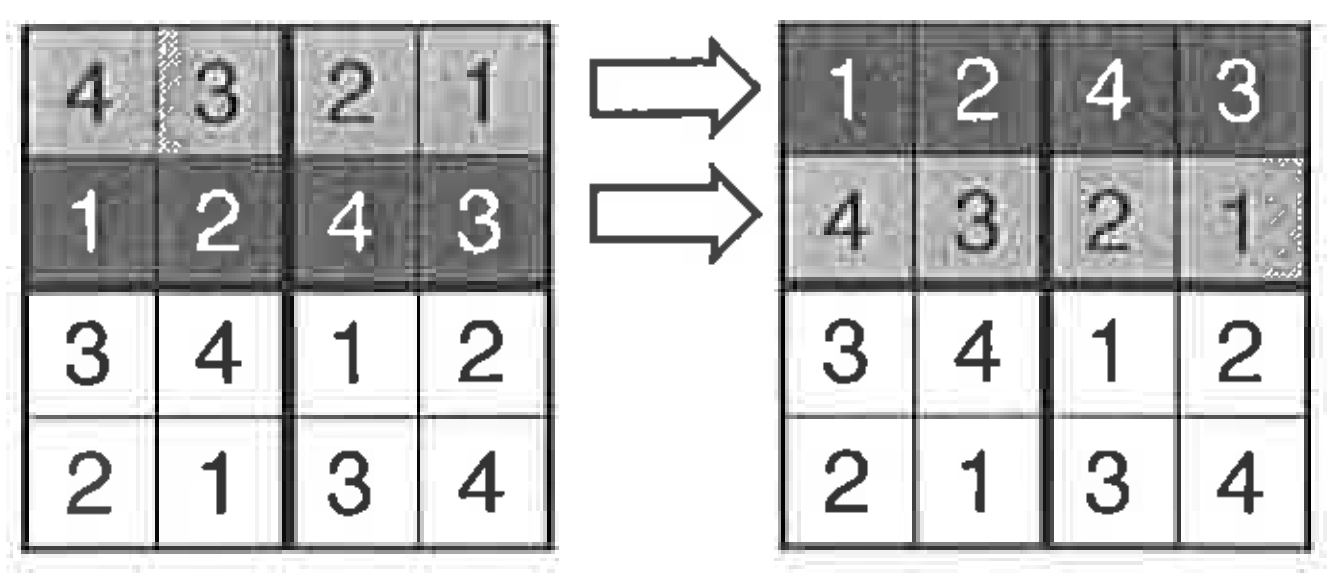
\includegraphics[width=0.3\paperwidth]{C:/Users/Admin/Desktop/Github/question_bank/LyX/static/img/9597-ALVL-2017-P1-Q4-1}\tabularnewline
\hline 
\textbf{2} & Swaps two columns in the same quadrants & \tabularnewline
 &  & 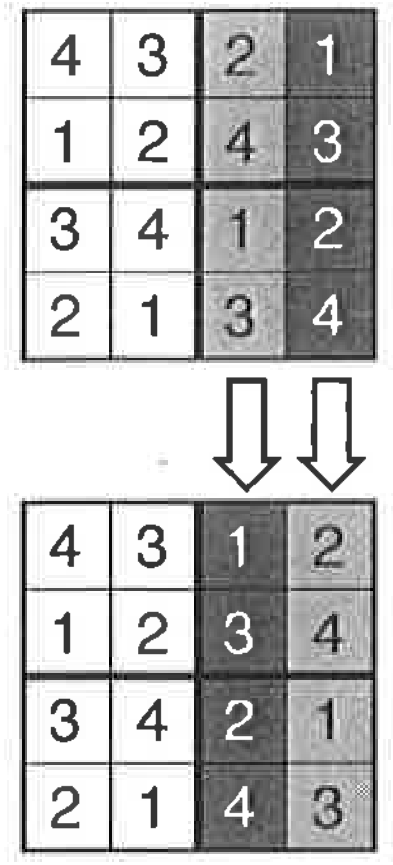
\includegraphics[width=0.15\paperwidth]{C:/Users/Admin/Desktop/Github/question_bank/LyX/static/img/9597-ALVL-2017-P1-Q4-2}\tabularnewline
\hline 
\textbf{3} & Swaps the top and bottom quadrant rows entirely & \tabularnewline
 &  & 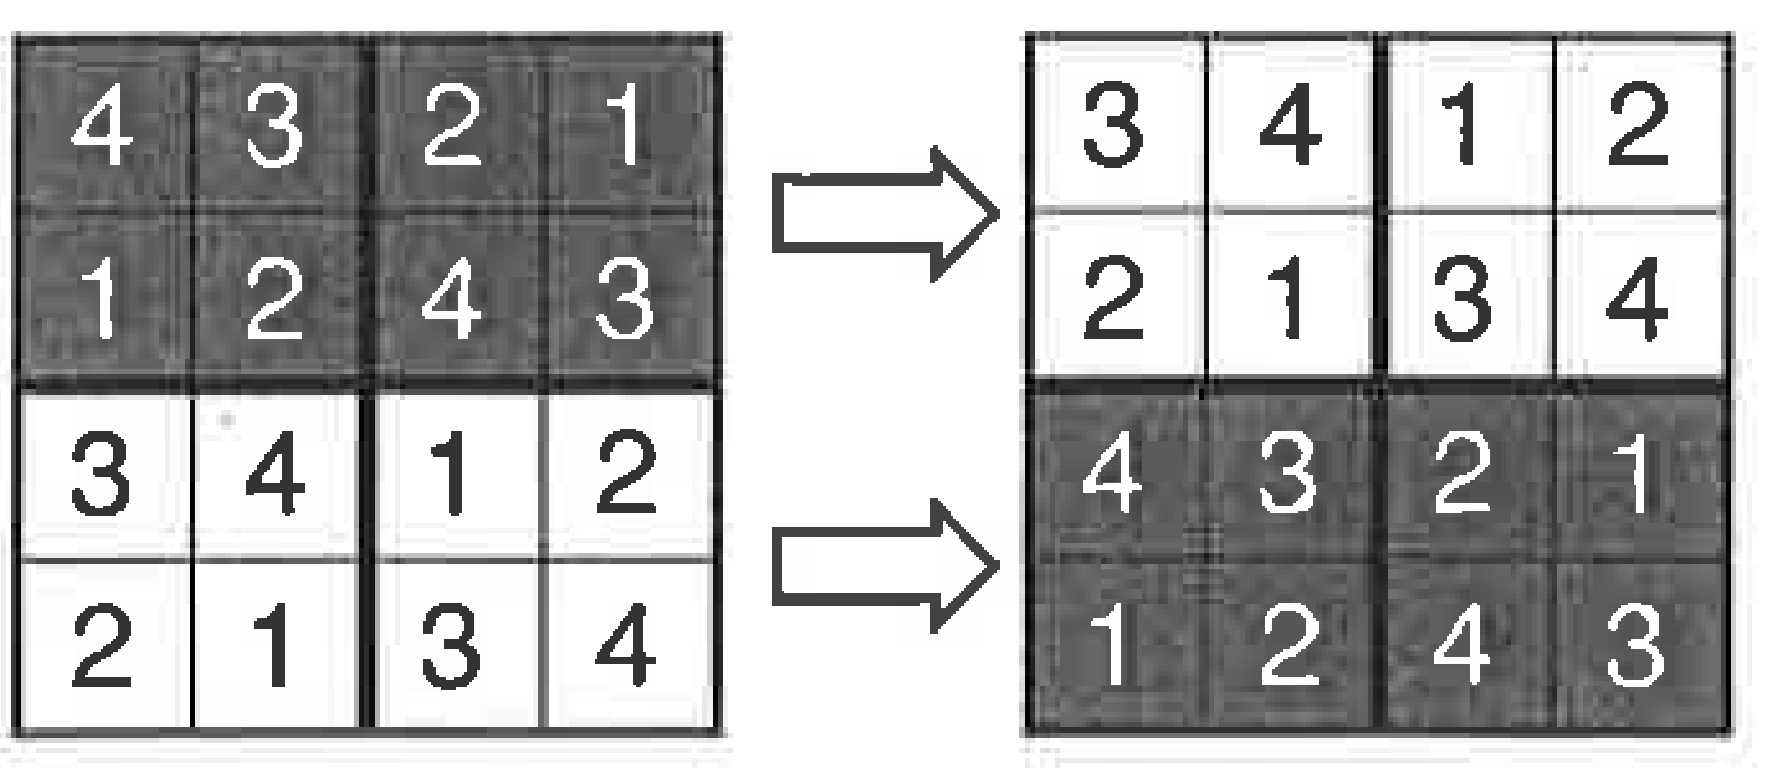
\includegraphics[width=0.3\paperwidth]{C:/Users/Admin/Desktop/Github/question_bank/LyX/static/img/9597-ALVL-2017-P1-Q4-3}\tabularnewline
\hline 
\textbf{4} & Swaps the left and right quadrant columns entirely & \tabularnewline
 &  & 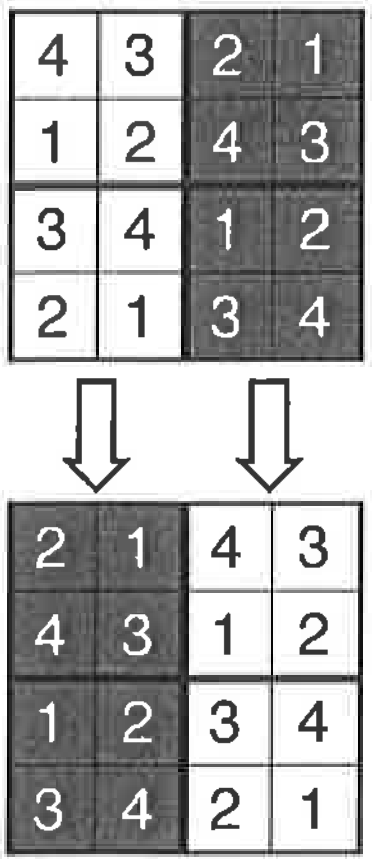
\includegraphics[width=0.15\paperwidth]{C:/Users/Admin/Desktop/Github/question_bank/LyX/static/img/9597-ALVL-2017-P1-Q4-4}\tabularnewline
\hline 
\end{tabular}
\par\end{center}

\subsubsection*{Task 4.3}

Write additional program code with brief \textbf{internal commentary}
to identify each transformation. 

The program code will: 
\begin{itemize}
\item create a method of selecting. at random, two of the four possible
transformations to be applied to the puzzle 
\item call a sub-program for each of the required transformations 
\item randomly select which rows will be transformed for transformations
1 and 2. for example. either the top or bottom two rows (for transformation
1) OR either the left-most or right-most two columns (for transformation
2) respectively 
\item display the puzzle before each transformation is applied and after
the final transformation. Before each transformation. it will also
display the name of the transformation being carried out. 

For example: 

\texttt{4321 }

\texttt{1243 }

\texttt{3412 }

\texttt{2134 }

\texttt{Transformation 1: Swaps two rows in the same quadrants }

\texttt{1243 }

\texttt{4321 }

\texttt{3412 }

\texttt{2134 }

\texttt{Transformation 4: Swaps the left and right quadrant columns
entirely }

\texttt{4312 }

\texttt{2143 }

\texttt{1234 }

\texttt{3421 }
\end{itemize}

\subsubsection*{Evidence 16}

Your program code that includes internal commentary.\hfill{} {[}14{]}

\subsubsection*{Evidence 17}

Screenshots of the output that shows each of the four transformations
applied. \hfill{}{[}4{]}

 \newpage 

\item \textbf{{[}ALVL/9597/2017/P2/Q1{]} }

The principal of a college decides to improve security access. Currently,
the staff use keys to enter classrooms and laboratories. One of the
principal\textquoteright s suggested improvements is to replace the
existing locks and keys with a swipe card system. The principal plans
to purchase swipe card readers for every room, and staff will be issued
with their own swipe card. if a valid card is swiped through a particular
reader, the corresponding door will be unlocked.

Software for controlling the system is required to: 
\begin{itemize}
\item define the rooms that can be entered by each card. The office staff
will make any changes. 
\item produce a pop-up screen on the office staff's computer if an unauthorised
card is used to attempt an entry into a room. 
\item produce reports. Some of the reports will be confidential and can
only be viewed by the principal. 
\end{itemize}
A local software company is selected to produce the software. The
company assigns a development team to the project. 
\begin{enumerate}
\item A systems analyst from the team makes an initial visit to the college. 

State two groups of staff that the systems analyst would need to interview.
Justify your answer. \hfill{}{[}4{]}
\item As a result of the analysis carried out. a diagram is used to show
entities and data flow. Draw a suitable diagram. \hfill{}{[}6{]}
\item The next stage of system development is software design.
\begin{enumerate}
\item Describe the checks that the team needs to make at the end of this
stage. \hfill{}{[}2{]}
\item Describe two methods that could be used to check this design. For
each method, identify the members of the development team involved
other than the systems analyst. {[}6{]}
\end{enumerate}
\item The swipe card system will need to be fully tested. The company carries
out white box and black box testing. 

Explain \textbf{three} differences between black box and white box
testing. \hfill{}{[}6{]}
\item User documentation will be produced during the development process. 

Describe \textbf{three} sections that should be included in the user
guide for this system.\hfill{} {[}6{]}
\item After the system is implemented, maintenance will be required. 

Name and describe \textbf{two} types of maintenance. For each type,
give an example for the swipe card system. \hfill{}{[}6{]}
\item Describe a method that can be used to ensure that only the office
staff can change the system and only the principal can view confidential
reports. \hfill{}{[}2{]}
\item The principal is considering expanding the use of the swipe card system
to record attendance in classes. 

Describe \textbf{one} disadvantage of this proposal and suggest a
more reliable method.\hfill{} {[}2{]}
\end{enumerate}

 \newpage 

\item \textbf{{[}ALVL/9597/2017/P2/Q2{]} }

A multinational company has many local branches in various parts of
the country that are linked using a wide area network (WAN). 
\begin{enumerate}
\item The company's network transfers data using asynchronous data transmission. 
\begin{enumerate}
\item State which of the following diagrams represents asynchronous data
transmission. Explain your answer. \hfill{}{[}2{]}
\begin{center}
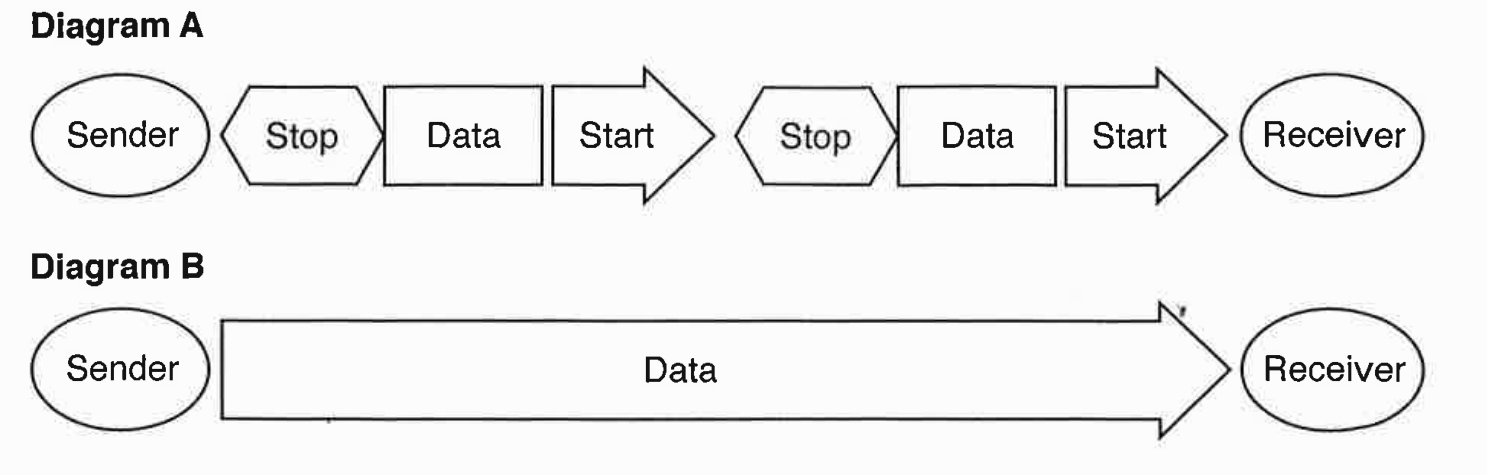
\includegraphics[width=0.5\paperwidth]{C:/Users/Admin/Desktop/Github/question_bank/LyX/static/img/9597-ALVL-2017-P2-Q2-1}
\par\end{center}
\item Explain why asynchronous data transmission affects network performance.\hfill{}
{[}2{]}
\end{enumerate}
\end{enumerate}
An employee works from home on her wireless laptop. The following
diagram shows the configuration of the employee's home network.
\begin{center}
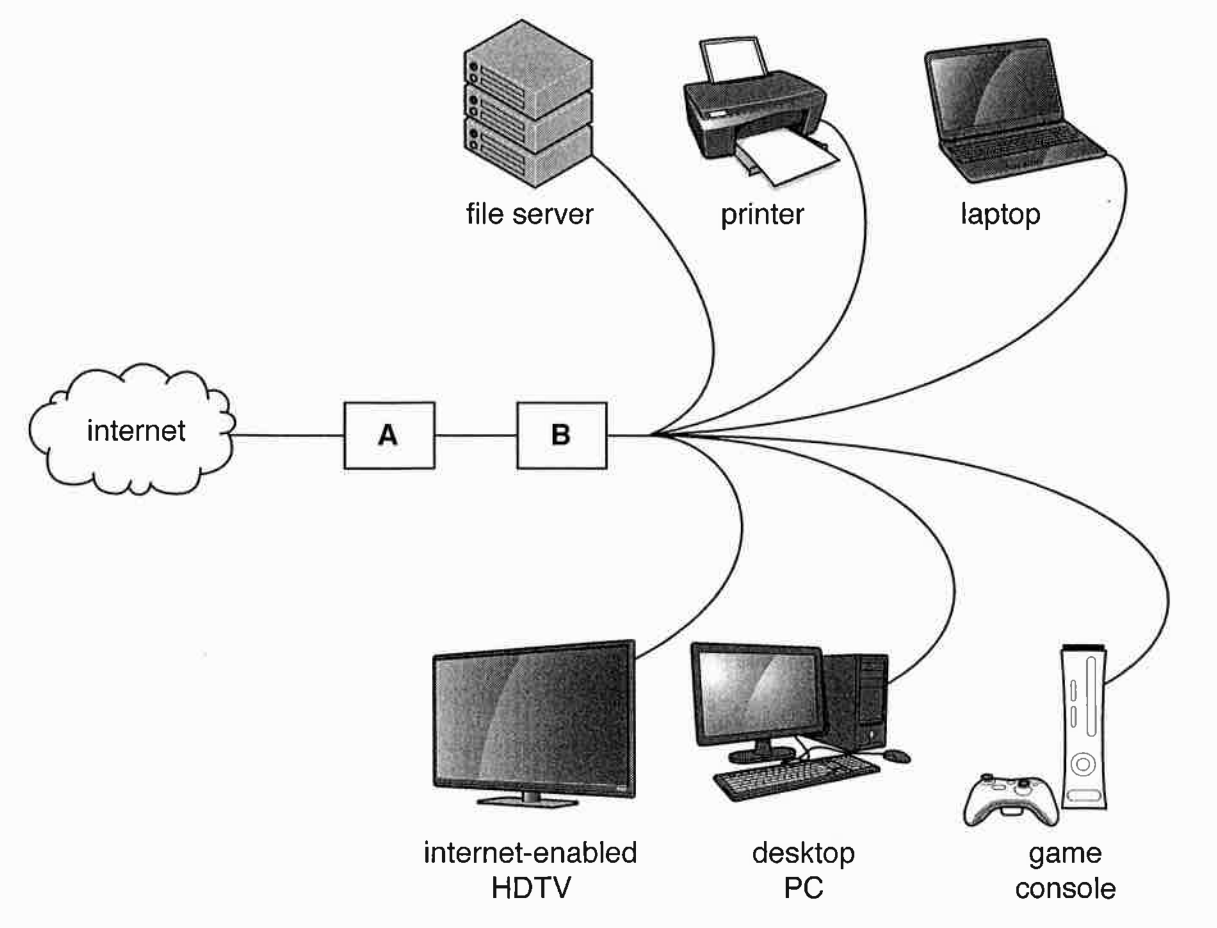
\includegraphics[width=0.5\paperwidth]{C:/Users/Admin/Desktop/Github/question_bank/LyX/static/img/9597-ALVL-2017-P2-Q2-2}
\par\end{center}
\begin{enumerate}
\item[(b)] This network uses both a switch and a router to transfer data. State
which of the pieces of equipment labelled \textbf{A} and \textbf{B}
is the switch. Explain your answer. \hfill{}{[}2{]}
\item[(c)] Describe \textbf{two} features of a router.\hfill{} {[}2{]}
\item[(d)] Describe \textbf{one} advantage and \textbf{one} disadvantage. for
the employee, of working from home.\hfill{} {[}2{]}
\end{enumerate}

 \newpage 

\item \textbf{{[}ALVL/9597/2017/P2/Q3{]} }
\begin{enumerate}
\item Explain what is meant by an object in object-oriented programming.
.\hfill{}{[}2{]} 
\item {} 
\begin{enumerate}
\item A student is writing a program to represent people in a university.
Tutors, office workers, lecturers and professors are all employed
by the university. A professor is a senior lecturer. The university
educates both undergraduate and graduate students. 

The student\textquoteright s program contains a class with the identifier
\texttt{Person}. Sub-classes share the characteristics of this class. 

Copy and complete the following inheritance diagram by adding sub-classes
\texttt{Professor}, 

\texttt{OfficeWorker}, \texttt{Lecturer}, \texttt{Undergraduate},
\texttt{Staff}, \texttt{Graduate}, \texttt{Student} and \texttt{Tutor}.
\hfill{}{[}2{]} 
\begin{center}
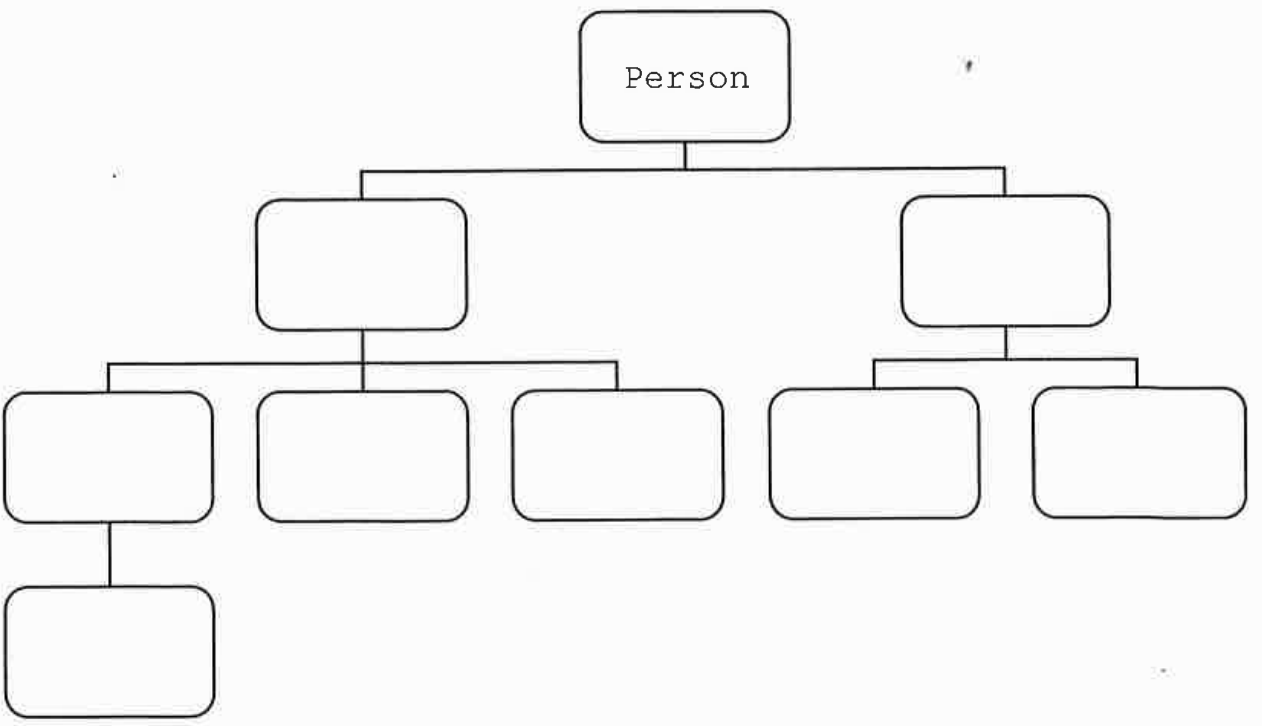
\includegraphics[width=0.5\paperwidth]{C:/Users/Admin/Desktop/Github/question_bank/LyX/static/img/9597-ALVL-2017-P2-Q3}
\par\end{center}
\item Explain why inheritance is an important feature of object-oriented
programming.\hfill{}{[}2{]} 
\end{enumerate}
\item A stack is a data structure that can be implemented in object-oriented
programming. The implementation of a stack requires an integer variable
and an array. 
\begin{enumerate}
\item Describe the purpose of the integer variable in the implementation
of a stack class.\hfill{} {[}1{]}
\item Describe the purpose of the array in the implementation of a stack
class.\hfill{} {[}1{]}
\item Explain how to use the stack data structure to compute the following
expression: 
\noindent \begin{center}
$\left(\text{A}+\text{B}\right)\times\left(\text{C}+\text{D}\right)$\hfill{}
{[}2{]}
\par\end{center}

\end{enumerate}
\end{enumerate}

 \newpage 

\item \textbf{{[}ALVL/9597/2017/P2/Q4{]} }
\begin{enumerate}
\item A local area network (LAN) can be set up as either client-server or
peer-to-peer. 
\begin{enumerate}
\item State where data are stored on a client-server network. \hfill{}
{[}1{]}
\item State where data are stored on a peer-to-peer network. \hfill{} {[}1{]}
\item Describe \textbf{one} benefit of a client-server network over a peer-to-peer
network. \hfill{} {[}2{]}
\item Describe \textbf{one} drawback of a client-server network compared
to a peer-to-peer network.\hfill{} {[}2{]}
\end{enumerate}
\item A college has five IT rooms. Each room has 20 computers which can
only print to a single printer in the room. At busy times in the year,
there can be up to 100 students printing their coursework at the same
time. \textquoteleft 0

Explain how all these print jobs are controlled and sent to the printer.\hfill{}
{[}2{]}
\item A 30 megabyte file is transferred over a network to a printer in 5
seconds. 

Calculate the transfer rate, in megabits per second, used to transfer
this file. Show all of your working. \hfill{} {[}2{]}
\end{enumerate}

 \newpage 

\item \textbf{{[}ALVL/9597/2017/P2/Q5{]} }The following grid shows the initial
state of a popular puzzle.
\begin{center}
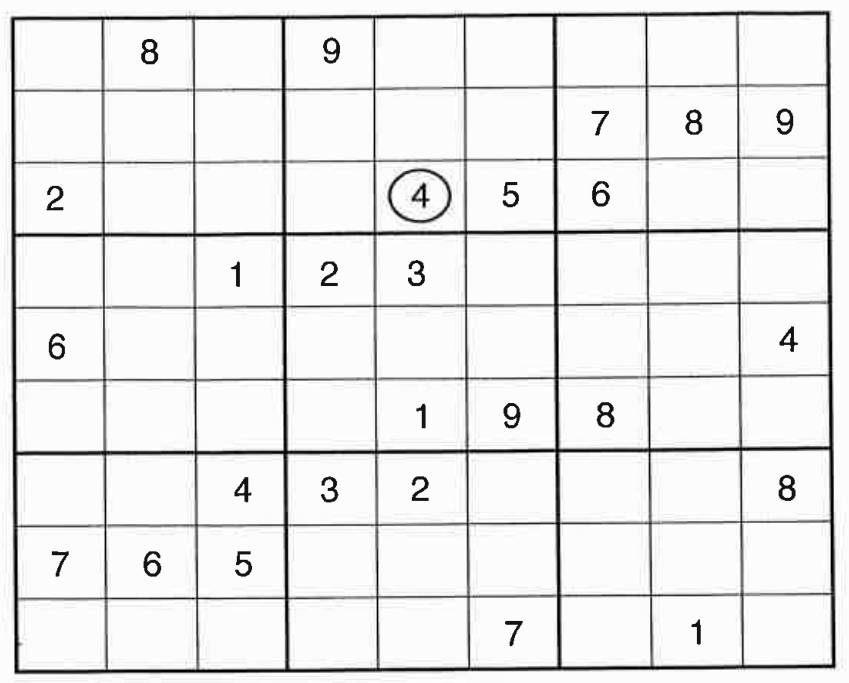
\includegraphics[width=0.5\paperwidth]{C:/Users/Admin/Desktop/Github/question_bank/LyX/static/img/9597-ALVL-2017-P2-Q5}
\par\end{center}

The aim of the puzzle is to fill the whole grid so that every row,
every column and every $3\times3$ mini-grid contains a number between
1 and 9. No number should be repeated in any row, column or 3 x 3
minigrid. 

A software company is creating an online version of the puzzle. A
programmer is asked to create the puzzle software. 
\begin{enumerate}
\item The programmer decides to use a 2D array to store the puzzle.
\begin{enumerate}
\item Copy and complete the following line of pseudocode. 

\texttt{DECLARE Puzzle ARRAY{[}1 : ...., .... : ....{]} OF ......................}
\hfill{}{[}2{]}

The circled value in the diagram above needs to be assigned to the
appropriate array element. 
\item Copy and complete the following line of pseudocode. 

\texttt{Puzzle{[}...., ....{]} <- ...............................}
\hfill{}{[}2{]}
\item Explain why a 2D array is more suitable than a single 1D array to
represent this puzzle. \hfill{}{[}2{]}
\end{enumerate}
\item The puzzle grid can be saved by writing the array \texttt{Puzzle}
to a file. 

Design an algorithm, using pseudocode, to write the array to the file.
\hfill{} {[}5{]}
\item During the testing of the puzzle software, several errors are discovered. 

Describe \textbf{two} debugging techniques that could be used to locate
these errors. \hfill{}{[}4{]}
\end{enumerate}

 \newpage 

\item \textbf{{[}ALVL/9597/2017/P2/Q6{]} }

A computer company has several offices throughout the country, each
with several salespersons. A record of the sales made by each salesperson
has been set up using a relational database. There is a minimum amount
of \$150 for each sale.

The following tables hold the data. 

\texttt{CUSTOMER (}\texttt{\uline{CustomerID}}\texttt{, CustomerName,
CustomerEmail, CustomerTelephone) }

\texttt{OFFICE (}\texttt{\uline{OfficeID}}\texttt{, Address, Telephone) }

\texttt{SALE (}\texttt{\uline{CustomerID{*}}}\texttt{, }\texttt{\uline{SalesPersonID{*}}}\texttt{,
SaleDate, Amount) }

\texttt{SALESPERSON (}\texttt{\uline{SalesPersonID}}\texttt{, SalespersonName,
OfficeID{*}) }

\textbf{Note:} underline indicates primary key. An asterisk ({*})
indicates a foreign key. 
\begin{enumerate}
\item Draw an Entity-Relationship (E-Fl) diagram to represent the data model.
\hfill{} {[}3{]} 
\item (b) The following is a section of the data dictionary for the data
model. it has three missing entries labelled \textbf{A}, \textbf{B
}and \textbf{C}.
\begin{center}
\begin{tabular}{|l|l|l|c|}
\hline 
\texttt{\textbf{\hspace{0.01\columnwidth}}}\textbf{Table} & \texttt{\textbf{\hspace{0.01\columnwidth}}}\textbf{Field} & \textbf{Data type} & \textbf{Validation}\tabularnewline
\hline 
\texttt{CUSTOMER} & \texttt{CustomerID} & Integer & Unique\tabularnewline
\hline 
\texttt{SALE} & \texttt{CustomerID} & Integer & \textbf{A}\tabularnewline
\hline 
\texttt{SALE} & \texttt{SaleData} & Date & \tabularnewline
\hline 
\texttt{SALE} & \texttt{Amount} & \texttt{\textbf{\hspace{0.01\columnwidth}}}\textbf{B} & \textbf{C}\tabularnewline
\hline 
\end{tabular}
\par\end{center}

State a suitable entry for \textbf{A}, \textbf{B} and \textbf{C}.
\hfill{}{[}3{]} 
\item There is an address field in this database.

Explain why storing the address as a single field is not good database
design. \hfill{}{[}3{]}
\end{enumerate}
Each month, a report is produced to show the sales for each salesperson.
The following is a report for salesperson, B Chin. 
\begin{center}
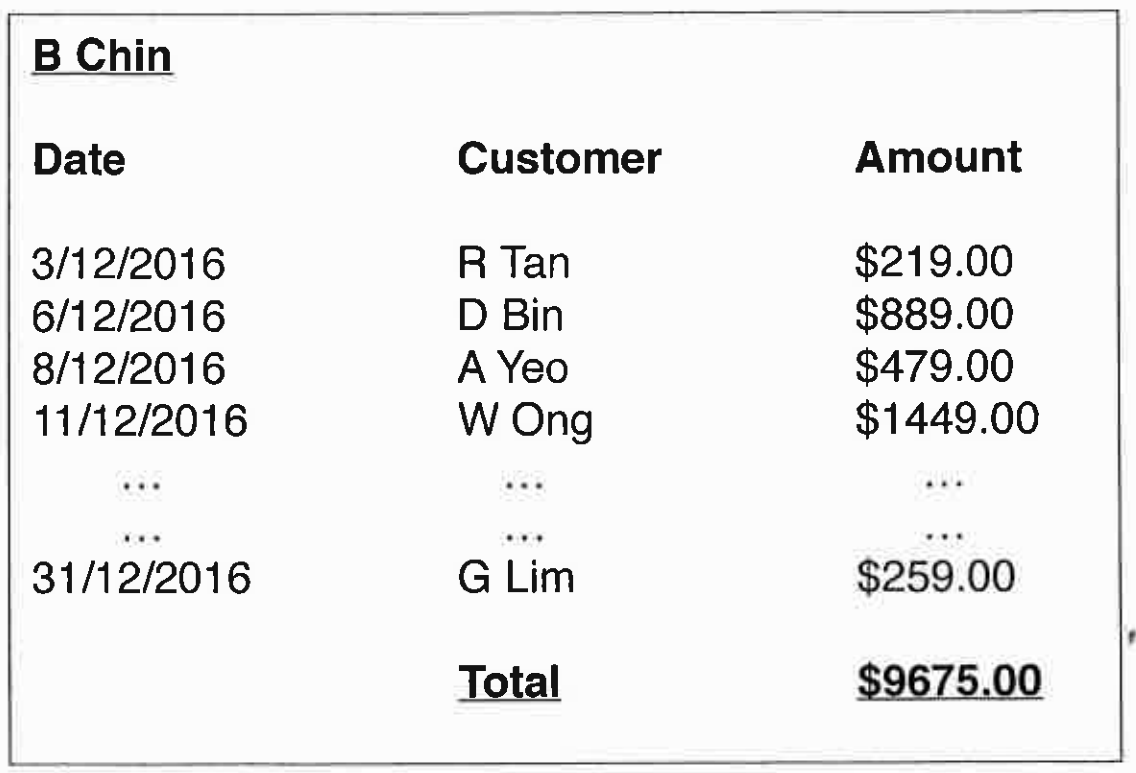
\includegraphics[width=0.5\paperwidth]{C:/Users/Admin/Desktop/Github/question_bank/LyX/static/img/9597-ALVL-2017-P2-Q6}
\par\end{center}
\begin{enumerate}
\item[(d)] {}
\begin{enumerate}
\item To produce the report, the database uses the \texttt{SaleDate} and
\texttt{Amount} fields in the \texttt{SALE} table. 

Name \textbf{four }other fields that the database uses to produce
this report.\hfill{} {[}4{]}
\item State \textbf{two} features of a relational database management system
which would be used to calculate and display the total for this salesperson.\hfill{}
{[}2{]}
\end{enumerate}
\end{enumerate}

 \newpage 

\item \textbf{{[}ALVL/9597/2018/P1/Q1{]} }

A program is required to input and process the number of steps taken
by members of a walking club each week. The number of steps taken
by each member is an integer in the range 0 to 100000. 

Each week, the \textquotedblleft Star of the Week\textquotedbl{} is
the member who has taken the greatest number of steps. 

The name and number of steps taken by the \textbf{previous} week's
\textquotedbl Star of the Week\textquotedbl{} are stored in the text
file, \texttt{STAR.TXT}. 

The program specification is as follows: 
\begin{itemize}
\item Input \textbf{up to} 10 names and the number of steps each has taken.
Assume that each number of steps is unique. 
\item Find the walker who has taken the greatest number of steps from this
data. 
\item Read the data about the previous \textquotedblleft Star of the Week\textquotedblright{}
from the text file \texttt{STAR. TXT}. 
\item Display a message on screen to show the previous star of the week
\textbf{and} the new star of the week, each with their number of steps.
For example, 

\texttt{Last week, Jenny Smith was 'Star of the Week' with 75827 steps
taken. }

\texttt{This week, Vanessa Lim is 'Star of the Week' with 67152 steps
taken. }
\item Update the text file, \texttt{STAR.TXT}, with the details of the new
\textquotedbl Star of the Week\textquotedblright . 
\end{itemize}

\subsubsection*{Task 1.1}

Write program code for this task that includes validation of data
entered.

\subsubsection*{Evidence 1}

Your program code. \hfill{}{[}8{]}

The program needs to be tested with different test cases. Consider
carefully, test cases for input of names and steps. 

\subsubsection*{Task 1.2}

Copy the table with the following headings. Add other test cases to
the table. One type of test case has already been added to the table.
\begin{center}
\begin{tabular}{|l|l|l|}
\hline 
\hspace{0.05\columnwidth}\textbf{Test case} & \textbf{Purpose of test data} & \textbf{Expected results}\tabularnewline
\hline 
Yi Ling Aw, 10232 & Test the maximum of 10 values & 10 values entered and star of\tabularnewline
Ryan Batisah, 42231 & entered into the program. & the week is Vanessa Lim with\tabularnewline
Lee Casmir, 35020 &  & 67152 steps taken.\tabularnewline
Daniel Bennett, 60192 &  & \tabularnewline
Sarah Heng Chee, 29389 &  & \tabularnewline
Vanessa Lim, 67152 &  & \tabularnewline
Wong Yip, 53231 &  & \tabularnewline
Rin Xie, 34200 &  & \tabularnewline
Tin Wee, 49480 &  & \tabularnewline
David Bala, 32010 &  & \tabularnewline
\hline 
\end{tabular}
\par\end{center}

\subsubsection*{Evidence 2}

Completed table with other test cases added. \hfill{}{[}4{]}

\subsubsection*{Task 1.3}

Use \textbf{three} of the test cases in the table, and produce a screenshot
for each.

\subsubsection*{Evidence 2}

Three screenshots of test cases.\hfill{}{[}3{]}

 \newpage 

\item \textbf{{[}ALVL/9597/2018/P1/Q2{]} }

The following algorithm is an implementation of a quick sort that
operates on an array \texttt{Scores}. 

This algorithm assumes that the first element of an array is the zeroth
element. This means that \texttt{Scores{[}0{]}} is the first element
in the array.

This pseudocode is available in the file \texttt{QUICKSORT.TXT}

\noindent\begin{minipage}[t]{1\columnwidth}%
\noindent \texttt{FUNCTION QuickSort(Scores)}

\noindent \texttt{\qquad{}QuickSortHelper(Scores, 0, LENGTH(Scores)
- 1)}

\noindent \texttt{\qquad{}RETURN Scores}

\noindent \texttt{ENDFUNCTION}

\bigskip{}

\noindent \texttt{FUNCTION QuickSortHelper(Scores, First, Last)}

\noindent \texttt{\qquad{}IF First < Last}

\noindent \texttt{\qquad{}THEN}

\noindent \texttt{\qquad{}\qquad{}SplitPoint <- PartitioniScores,
First, Last)}

\noindent \texttt{\qquad{}\qquad{}QuickSortHelper(Scores, First,
SplitPoint \textemdash{} 1)}

\noindent \texttt{\qquad{}\qquad{}QuickSoRtHelper(Scores, SplitPoint
+ 1, Last)}

\noindent \texttt{\qquad{}ENDIF}

\noindent \texttt{\qquad{}RETURN Scores}

\noindent \texttt{ENDFUNCTION }\bigskip{}

\noindent \texttt{FUNCTION Partition(Scores, First, Last)}

\noindent \texttt{\qquad{}PivotValue <- ScoresiFirst{]}}

\noindent \texttt{\qquad{}Lefthark <- First + 1}

\noindent \texttt{\qquad{}RightMark <- Last}

\noindent \texttt{\qquad{}Done <- FALSE}

\noindent \texttt{\qquad{}WHILE (Done = FALSE)}

\noindent \texttt{\qquad{}\qquad{}WHILE LeftMark <= RightMark AND
Scores{[}LeftMark{]} <= PivotValue}

\noindent \texttt{\qquad{}\qquad{}\qquad{}LeftMark <- LeftMark
+ 1}

\noindent \texttt{\qquad{}\qquad{}ENDWHILE}

\noindent \texttt{\qquad{}\qquad{}WHILE Scores{[}RightMark{]} >=
PivotValue AND RightMark >= LeftMark}

\noindent \texttt{\qquad{}\qquad{}\qquad{}RightMark <- RightMark
\textemdash{} 1}

\noindent \texttt{\qquad{}\qquad{}ENDWHILE}

\noindent \texttt{\qquad{}\qquad{}IF RightMark < LeftMark}

\noindent \texttt{\qquad{}\qquad{}\qquad{}THEN}

\noindent \texttt{\qquad{}\qquad{}\qquad{}\qquad{}Done <- TRUE}

\noindent \texttt{\qquad{}\qquad{}ELSE}

\noindent \texttt{\qquad{}\qquad{}\qquad{}Temp <- Scores{[}LeftMark{]}}

\noindent \texttt{\qquad{}\qquad{}\qquad{}Scores{[}LeftMark{]}
<- Scores{[}RightMark{]}}

\noindent \texttt{\qquad{}\qquad{}\qquad{}Scores{[}RightMark{]}
<- Temp}

\noindent \texttt{\qquad{}ENDIF}

\noindent \texttt{ENDWHILE }\bigskip{}

\noindent \texttt{\textbf{\emph{<swap Scores{[}First{]} with Scores{[}RightMark{]}>}}}\texttt{
}\bigskip{}

\noindent \texttt{\qquad{}RETURN RightMark}

\noindent \texttt{ENDFUNCTION}%
\end{minipage}

\subsubsection*{Task 2.1}

Write program code to implement this algorithm. Ensure that you add
the missing code to complete the algorithm. The area of missing code
is highlighted as:
\begin{center}
\texttt{\textbf{\emph{<swap Scores {[}First{]} with Scores {[}RightMark{]}>}}}
\par\end{center}

Copy the sample data available in the \texttt{SCORES.TXT} file. Paste
this into your programming code to set up the data to be sorted.

\subsubsection*{Evidence 4}

Your program code. \hfill{}{[}12{]}

\subsubsection*{Task 2.2}

Add a function to your code to output Scores. Call this function before
and after the operation of the quick sort so that the unsorted and
sorted data is displayed.

\subsubsection*{Evidence 5}

Your program code. \hfill{}{[}2{]}

\subsubsection*{Evidence 6}

Screenshot showing the unsorted and sorted \texttt{Scores} data.\hfill{}
{[}1{]}

 \newpage 

\item \textbf{{[}ALVL/9597/2018/P1/Q3{]} }

The file,\texttt{ HASHEDDATA.TXT}, holds details of the names and
telephone numbers of 250 people. 

There are a total of 500 lines in the file, and a number of these
lines are empty of name and telephone number.

An index is stored for each line of the file. 

The format of the data in the file is: 
\begin{center}
<Index>,<PersonName>,<TelephoneNumber> 
\par\end{center}

The first 10 lines from the file are shown as follows: 

\noindent\fbox{\begin{minipage}[t]{1\columnwidth - 2\fboxsep - 2\fboxrule}%
0, ,

1, ,

2, ,

3, Boon Keng V., 07492 546415

4, ,

5, ,

6, Ahmad Yusof, 07439 778665

7, Durno Peter, 07662 863518

8, Batisah Wong, 07362 156265

9, ,%
\end{minipage}}

The values in the file are separated by the comma character. 

A record structure is used to store a name and telephone number. A
data structure of 500 records is needed to store all the names and
telephone numbers. Each line in the file is written to a corresponding
position in the data structure.

The records with index six to eight from the data structure are: 
\begin{center}
\begin{tabular}{r|c|c|}
\cline{2-3} \cline{3-3} 
\textbf{Index} & \textbf{PersonName} & \textbf{TelephoneNumber}\tabularnewline
\cline{2-3} \cline{3-3} 
6 & Ahmad Yusof & 07439 778665\tabularnewline
\cline{2-3} \cline{3-3} 
7 & Durno Peter & 07662 863518\tabularnewline
\cline{2-3} \cline{3-3} 
\texttt{8} & Batisah Wong & 07362 156265\tabularnewline
\cline{2-3} \cline{3-3} 
\end{tabular}
\par\end{center}

\subsubsection*{Task 3.1}

Use program code to create a:
\begin{itemize}
\item record structure to hold the name and telephone number for one person
\item data structure, using this record structure to store 500 records.
\end{itemize}

\subsubsection*{Evidence 7}

Your program code. \hfill{}{[}6{]}

\subsubsection*{Task 3.2}

Write program code to:
\begin{itemize}
\item read the lines from the file
\item extract the <Index>, <PersonName> and <TelephoneNumber> values
\item store these values in the data structure.
\end{itemize}
Create a procedure called \texttt{DisplayValues} that will loop though
the data structure and display the index, name and telephone number
for every record where the name is present.

Ensure your procedure uses headings to identify the data displayed.

\subsubsection*{Evidence 8}

Your program code. \hfill{}{[}13{]}

\subsubsection*{Evidence 9}

A Screenshot showing the output.\hfill{} {[}1{]}

A hashing function was used to create the file. The same hashing function
can be used to search the data structure for a particular name. The
hashing function generates a hash. This is calculated as follows:

\noindent\begin{minipage}[t]{1\columnwidth}%
\texttt{Get SearchName}

\texttt{Set HashTotal to 0}

\texttt{FOR each Character in SearchName}

\texttt{\qquad{}Get the ASCII code for Character}

\texttt{\qquad{}Multiply the ASCII code by the position of Character
in SearchName}

\texttt{\qquad{}Add the result to the HashTotal}

\texttt{Calculate Hash as HashTotal MOD 500}

\texttt{RETURN Hash}%
\end{minipage}

\subsubsection*{Task 3.3}

Add the program code for the hashing function. Use the following specification:
\begin{center}
\texttt{FUNCTION GenerateHash(SearchName : STRING) : INTEGER}
\par\end{center}

The function has a single parameter \texttt{SearchName} and returns
an integer value.

Write additional code for your program to allow you to test the implementation
of this function.

The following test data will assist you.

\qquad{}\textquotedblleft Tait Davinder\textquotedblright{} should
return a hash of 87

\qquad{}\textquotedblleft Anandan Yeo\textquotedbl{} should return
a hash of 156

\subsubsection*{Evidence 10}

Your program code. \hfill{}{[}8{]}

\subsubsection*{Evidence 11}

A screenshot (or screenshots) of your program to show the results
of the hash calculation for both the given test data values.\hfill{}{[}2{]}

The hash calculated from the \texttt{SearchName} can be used to find
a corresponding record in the data structure.

If the \texttt{SearchName} is not found in the record given by the
hash \textbf{and} the record is not empty:
\begin{itemize}
\item compare \texttt{SearchName} with the next record
\item until the \texttt{SearchName} is found or an empty record is found.
\end{itemize}
If an empty record is found then the program will report that the
name is \textquotedblleft NOT FOUND\textquotedblright .

If the record is found, the program will output the index, name and
telephone number.

\subsubsection*{Task 3.4}

Add the program code to implement the search as described.

\subsubsection*{Evidence 12}

Your program code. \hfill{}{[}7{]}

\subsubsection*{Evidence 11}

A screenshot (or screenshots) of your program to show the results
of the following searches:

Search 1: Charlie Love

Search 2: Chin Tan

Search 3: John Barrowman\hfill{}{[}3{]}

 \newpage 

\item \textbf{{[}ALVL/9597/2018/P1/Q4{]} }

In a computer game, a player (\textquotedbl\texttt{O}\textquotedbl )
moves around a maze measuring 10 metres by 11 metres to collect a
prize (\textquotedbl\texttt{P}\textquotedbl ). The prize is placed
at a random position within the maze. The prize position is not where
a wall (\textquotedbl\texttt{X}\textquotedbl ) appears in the maze.
An empty position is indicated with a full-stop (\textquotedbl\texttt{.}\textquotedbl ). 

The maze is represented on the screen by a rectangular grid. Each
square metre of the maze is represented by an x-coordinate and a y-coordinate.
The top left square metre of the puzzle display has x = \texttt{0}
and y = \texttt{0}.

The player moves left, right, up or down according to a direction
entered by the user. The game is turn-based; a user enters the direction,
their player moves one position in that direction. lithe direction
would place the player on a well, then the player does not move. The
maze is displayed after each move.
\begin{center}
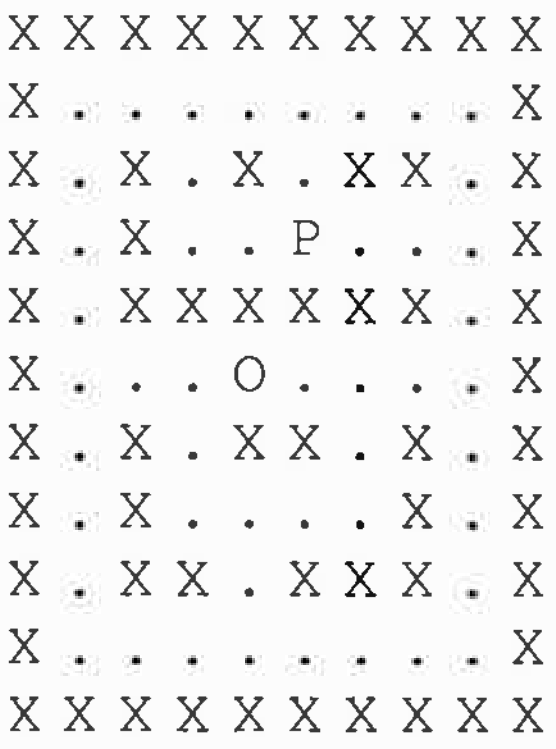
\includegraphics[width=0.25\paperwidth]{C:/Users/Admin/Desktop/Github/question_bank/LyX/static/img/9597-ALVL-2018-P1-Q4}
\par\end{center}

\subsubsection*{Task 4.1}

Write a program to display the maze as shown.
\begin{itemize}
\item The maze should be stored in a suitable data structure.
\item The data structure will allow fixed loop(s) to be used to display
the maze.
\end{itemize}
The maze is given in the text file \texttt{MAZE.TXT}. You may read
in the data from this file or place the data in your program using
any suitable method.

\subsubsection*{Evidence 14}

Your program code. \hfill{} {[}6{]}

\subsubsection*{Task 4.2}

The prize is placed randomly on the maze. It cannot appear in the
same grid position as a wall (\textquotedbl\texttt{X}\textquotedbl ).

Add to your program code to place the prize at a random position.

Take a screenshot of the maze with the prize displayed in it.

\subsubsection*{Evidence 15}

Your program code. \hfill{}{[}4{]}

\subsubsection*{Evidence 16}

A screenshot of the maze as output by your program. \hfill{} {[}1{]}

The player is represented by the character \textquotedbl\texttt{O}\textquotedbl .
The character starts the game in a central position on the grid, for
example, x = \texttt{4} and y = \texttt{5}. 

To move the character, the user is prompted for a direction. The following
are valid inputs:
\begin{center}
\begin{tabular}{|c|l|}
\hline 
\textbf{Input character} & \hspace{0.05\columnwidth}\textbf{Action}\tabularnewline
\hline 
\texttt{``U''} & Player moves up\tabularnewline
\hline 
\texttt{``D''} & Player moves down\tabularnewline
\hline 
\texttt{``L''} & Player moves left\tabularnewline
\hline 
\texttt{``R''} & Player moves right\tabularnewline
\hline 
\texttt{``''} & Continue with previous move.\tabularnewline
 & If no previous move, do nothing\tabularnewline
\hline 
\end{tabular}
\par\end{center}

If the next position for the player (\textquotedbl\texttt{O}\textquotedbl )
is a wall (\textquotedbl\texttt{X}\textquotedbl ), then the player
stays in their current position; this is called collision detection.

When the player enters the move, a new position for the player (\textquotedbl\texttt{O}\textquotedbl )
is calculated and the maze is displayed. The previous position is
changed back to a \textquotedbl .\textquotedbl{} when the player
has a new position. The moves are repeated until the player is at
the same position as the prize.

\subsubsection*{Task 4.3}

Add to your program code to:
\begin{itemize}
\item place the player on the grid at a central position on the grid
\item take in and validate a direction
\item calculate a new position
\item check this position is not a wall
\item update the grid so that the previous position of \textquotedbl\texttt{O}\textquotedbl{}
is replaced with a \textquotedbl{} . \textquotedbl{} and \textquotedbl\texttt{O}\textquotedbl{}
is located in its new position
\item continue this until the player is at the same position as the prize.
\end{itemize}

\subsubsection*{Evidence 17}

Your program code. \hfill{} {[}16{]}

When the player and the prize are at the same position, the message
\textquotedblleft Player has reached the prize\textquotedblright{}
is displayed and the game ends.

\subsubsection*{Task 4.4}

Add to your program, code to end the game when this condition is met,
and display the required message. Produce screenshots to show key
elements of your program are functioning.

The screenshots required are:
\begin{itemize}
\item entering each direction
\item player changing position
\item end of game
\end{itemize}

\subsubsection*{Evidence 18}

Your program code. \hfill{} {[}1{]}

\subsubsection*{Evidence 19}

Screenshots of:
\begin{itemize}
\item entering each direction
\item player changing position
\item end of game (player wins) \hfill{} {[}2{]}
\end{itemize}

 \newpage 

\item \textbf{{[}ALVL/9597/2018/P2/Q1{]} }

A mobile phone company has an option for Pay As You Go usage. Customers
have to purchase credit in advance. The credit is used to pay for
texts, calls and data. Customers can buy additional credit at any
time. 

The company requires software to allow their Pay As You Go customers
to do the following tasks online: 
\begin{itemize}
\item check credit balance 
\item check data usage 
\item check call usage 
\item pay for credit 
\end{itemize}
A software company was employed to put together a project team to
produce the software. 
\begin{enumerate}
\item State \textbf{three} members of the project team. Describe the role
of each of these members. \hfill{}{[}6{]}
\item The initial phase of the system development cycle required that a
specification be created for the system. 
\begin{enumerate}
\item State \textbf{two} techniques that could have been used to gather
the information for this specification. \hfill{} {[}2{]}
\item Explain how each technique would have been used in this project. \hfill{}
{[}4{]}
\end{enumerate}
\item The specification is a detailed report.

Describe \textbf{two} sections of this report. \hfill{}{[}4{]}
\item The software could have been designed using different techniques. 
\begin{enumerate}
\item Name \textbf{and} describe \textbf{two} design techniques that may
have been used. \hfill{} {[}4{]}
\item Explain why it is important for each member of the design team to
use the same technique. \hfill{} {[}2{]}
\item A customer's mobile phone number needs to be validated on entry. 

Draw a flowchart to represent an algorithm for this validation. \hfill{}
{[}4{]}
\end{enumerate}
\item (e) The work to implement the new software needs to be managed. The
following Program Evaluation and Review Technique (PERT) chart is
used as a management tool. 

\texttt{A} --- Specification 

\texttt{B} --- Analysis 

\texttt{C} --- Design of software 

\texttt{D} --- Design of Interface 

\texttt{E} --- Documentation 

\texttt{F}--- Implementation 

\texttt{G} --- Testing 

\texttt{H} --- Acceptance testing

\texttt{I} --- Hand over to phone company 

Time is measured in weeks. 
\begin{center}
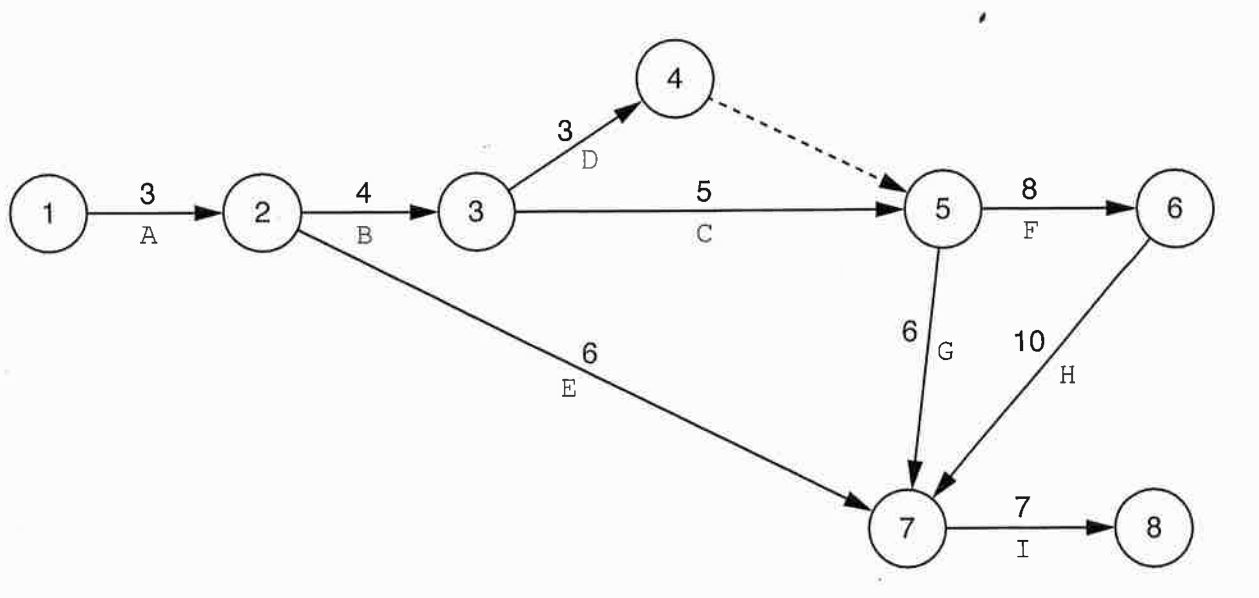
\includegraphics[width=0.5\paperwidth]{C:/Users/Admin/Desktop/Github/question_bank/LyX/static/img/9597-ALVL-2018-P2-Q1}
\par\end{center}
\begin{enumerate}
\item State the critical path for the given activities \texttt{A} to \texttt{I}.
\hfill{}{[}2{]}
\item Calculate the minimum time these activities will take. \hfill{}{[}1{]}
\item The member of the project team who worked on activity 0 fold the project
manager he could not start work until one week after the scheduled
start date. 

Explain any impact this would have on the completion date of the project.\hfill{}
{[}3{]}
\end{enumerate}
\item The software is intended for use on hand-held devices. 

Describe \textbf{two} ways that users can keep their data secure on
these devices.\hfill{} {[}4{]}
\item A member of the project team had the task of ensuring that social
and ethical issues were considered. 

Describe \textbf{one} example of each of these Issues that this member
of the team might have considered. \hfill{}{[}4{]}
\end{enumerate}

 \newpage 

\item \textbf{{[}ALVL/9597/2018/P2/Q2{]} }

The following algorithm calculates the average mark for a group of
students. 

\noindent\begin{minipage}[t]{1\columnwidth}%
\texttt{01 FOR Counter <- 1 TO NumberOfStudents}

\texttt{02 \qquad{}Total <- O}

\texttt{03 \qquad{}INPUT Mark}

\texttt{04 \qquad{}Total <- Total + Mark}

\texttt{05 ENDFOR}

\texttt{06 Average <- Total / NumberOfStudents}

\texttt{07 OUTPUT Average}%
\end{minipage}
\begin{enumerate}
\item There is an error in this algorithm causing an incorrect result. Describe
the error and explain the change required to correct this error. \hfill{}{[}3{]}
\item State the name of this type of error.\hfill{} {[}1{]}
\item The lowest mark in the exam is 0 and the highest is 100. Give an example
from each of the appropriate test cases which could be used to test
the algorithm. \hfill{}{[}4{]}
\item Name and describe a suitable technique that could be used to manually
identify errors in the algorithm. \hfill{}{[}2{]}
\end{enumerate}

 \newpage 

\item \textbf{{[}ALVL/9597/2018/P2/Q3{]} }
\begin{enumerate}
\item A binary tree is as follows: 
\begin{center}
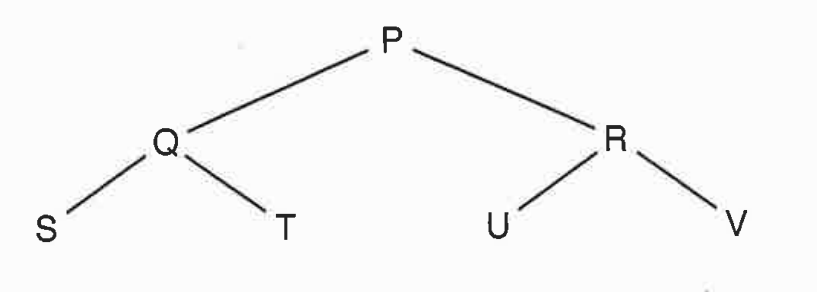
\includegraphics[width=0.5\paperwidth]{C:/Users/Admin/Desktop/Github/question_bank/LyX/static/img/9597-ALVL-2018-P2-Q3}
\par\end{center}
\begin{enumerate}
\item State the in-order sequence. \hfill{}{[}1{]}
\item State the pre-order sequence. \hfill{} {[}1{]}
\end{enumerate}
\item A 1D array, \texttt{Value}, stores a list of scores as follows:
\begin{center}
\begin{tabular}{|c|c|c|c|c|c|c|c|c|c|c|c|c|c|c|c|}
\hline 
Index & 0 & 1 & 2 & 3 & 4 & 5 & 6 & 7 & 8 & 9 & 10 & 11 & 12 & 13 & 14\tabularnewline
\hline 
Score & 2 & 6 & 15 & 23 & 36 & 48 & 50 & 58 & 64 & 69 & 74 & 79 & 86 & 92 & 99\tabularnewline
\hline 
\end{tabular}
\par\end{center}
\begin{enumerate}
\item Using a linear search, state how many comparisons will be required
to find the score of 64. \hfill{}{[}1{]}
\end{enumerate}
The following binary search algorithm could be used to search the
list of scores.

\noindent\begin{minipage}[t]{1\columnwidth}%
\texttt{01 Lower <- LowestIndex}

\texttt{02 Upper <- HighestIndex}

\texttt{03 REPEAT}

\texttt{04 \qquad{}Middle <- (Lower + Upper) DIV 2}

\texttt{05 \qquad{}IF SearchItem > Value{[}Middle{]}}

\texttt{O6 \qquad{}THEN}

\texttt{07 \qquad{}\qquad{}Lower <- Middle + l}

\texttt{08 \qquad{}ELSE}

\texttt{09 \qquad{}\qquad{}Upper <- Middle \textemdash{} l}

\texttt{10 \qquad{}ENDIF}

\texttt{11 UNTIL Value{[}Middle{]} = SearchItem OR Lower > Upper}

\texttt{12 OUTPUT \textquotedbl Score found at position\textquotedbl{}
Middle}%
\end{minipage}
\begin{enumerate}
\item[ii.] Score 80 is not in the list.

When searching for this score, state the values that will be examined.
\hfill{}{[}2{]}
\item[iii.] When searching for a score of 80, this algorithm outputs:

\texttt{Score found at position 12}

Describe how the algorithm gives this incorrect output. \hfill{}{[}2{]}
\item[iv.] Describe how the algorithm could be changed to give a suitable message
if the score is not in the list. \hfill{}{[}3{]}
\end{enumerate}
\end{enumerate}

 \newpage 

\item \textbf{{[}ALVL/9597/2018/P2/Q4{]} }

A university allows students to access the university network from
home. 
\begin{enumerate}
\item The university server has a firewall.

Describe \textbf{two} ways that a firewall can be used to block unauthorised
access to the network. \hfill{}{[}2{]}
\item The university wishes to restrict access to inappropriate websites
from within its network.

Describe \textbf{two} methods that could be used to restrict access
to inappropriate websites. \hfill{}{[}4{]}
\item The university is concerned about the possible loss of data from their
local servers.

Describe a strategy that could be used to prevent data loss. \hfill{}{[}2{]}
\item The university has its own intranet.

Describe \textbf{two} benefits that the intranet might provide for
students. \hfill{}{[}2{]}
\end{enumerate}

 \newpage 

\item \textbf{{[}ALVL/9597/2018/P2/Q5{]} }

The organisers of a diving championship have created software to calculate
and show the total score for each diver. 

There are nine judges scoring each dive. The two best scores and the
two worst scores are ignored. The other five scores are added together
to give the diver\textquoteright s total score. 
\begin{enumerate}
\item Write an algorithm to take in the nine scores, delete the best two
and the two worst scores, and total the five remaining scores. \hfill{}{[}4{]}
\end{enumerate}
There are 10 divers in the final. The scoreboard shows the order of
diving. 
\begin{center}
\begin{tabular}{|c|c|l|}
\hline 
\textbf{Order} & \textbf{Diver name} & \textbf{Total score}\tabularnewline
\hline 
1 & Daniel Tan & \tabularnewline
\hline 
2 & Parker Lam & \tabularnewline
\hline 
3 & Mohamed Noor & \tabularnewline
\hline 
4 & Hariz Yazid & \tabularnewline
\hline 
5 & Sheryl Xuan & \tabularnewline
\hline 
6 & Karl Lim & \tabularnewline
\hline 
7 & Elaine Ning & \tabularnewline
\hline 
8 & Nadyia Esmadi & \tabularnewline
\hline 
9 & Cai Ng & \tabularnewline
\hline 
10 & Hamid Mahmood & \tabularnewline
\hline 
\end{tabular}
\par\end{center}
\begin{enumerate}
\item The programmers decided to use a 1D array for the scores. They will
also use a bubble sort to sort the scores into descending order.
\begin{enumerate}
\item Explain how a bubble sort can be used to arrange the scores into a
descending or ascending order. \hfill{}{[}2{]}
\end{enumerate}
This is the bubble sort algorithm for sorting into descending order:

\noindent\begin{minipage}[t]{1\columnwidth}%
\texttt{01 WHILE NoSwaps = FALSE}

\texttt{02 \qquad{}NoSwaps <- TRUE}

\texttt{03 \qquad{}UpperBound <- ListLength}

\texttt{04 \qquad{}FOR Posn <- 0 TO ......}\texttt{\textbf{A}}\texttt{......}

\texttt{05 \qquad{}\qquad{}IF List{[}Posn{]} < ......}\texttt{\textbf{B}}\texttt{......}

\texttt{06 \qquad{}\qquad{}\qquad{}THEN}

\texttt{O7 \qquad{}\qquad{}\qquad{}\qquad{}// Swap}

\texttt{O8 \qquad{}\qquad{}\qquad{}\qquad{}NoSwaps <- ......}\texttt{\textbf{C}}\texttt{......}

\texttt{09 \qquad{}\qquad{}\qquad{}\qquad{}Temp <- List{[}Posn{]}}

\texttt{10 \qquad{}\qquad{}\qquad{}\qquad{}List{[}Posn{]} <- ListiPosn
+ 1{]}}

\texttt{11 \qquad{}\qquad{}\qquad{}\qquad{}List{[}Posn + 1{]}
<- ......}\texttt{\textbf{D}}\texttt{......}

\texttt{12 \qquad{}\qquad{}ENDIF}

\texttt{l3 \qquad{}ENDFOR}

\texttt{14 ENDWHILE}%
\end{minipage}
\begin{enumerate}
\item Write the pseudocode for \texttt{\textbf{A}}, \texttt{\textbf{B}},
\texttt{\textbf{C}}\textbf{ a}nd \texttt{\textbf{D}} in the algorithm.
\hfill{} {[}4{]}
\end{enumerate}
\item During the first round of dives, the sorted scores for five divers
are: 

\texttt{48 }

\texttt{45 }

\texttt{40 }

\texttt{37 }

\texttt{36 }

The sixth diver scores 42 and the software appends the score to the
list as follows: 

\texttt{48 }

\texttt{45 }

\texttt{40 }

\texttt{37 }

\texttt{36 }

\texttt{42}
\begin{enumerate}
\item State the number of passes needed through the list to return the list
to its sorted order. \hfill{}{[}1{]}
\item Explain why the bubble sort is efficient in this example. \hfill{}{[}2{]}
\item Name another sort method that could have been used in this situation. 

Compare the speed of sorting the divers\textquoteright{} scores in
your named method with using the bubble sort. \hfill{}{[}2{]}
\end{enumerate}
\end{enumerate}

 \newpage 

\item \textbf{{[}ALVL/9597/2018/P2/Q6{]} }

Customers want to buy tickets for a diving championship that takes
place over three days. There are two sessions of diving each day. 

Customers use a ticket ordering website to buy their tickets.
\begin{center}
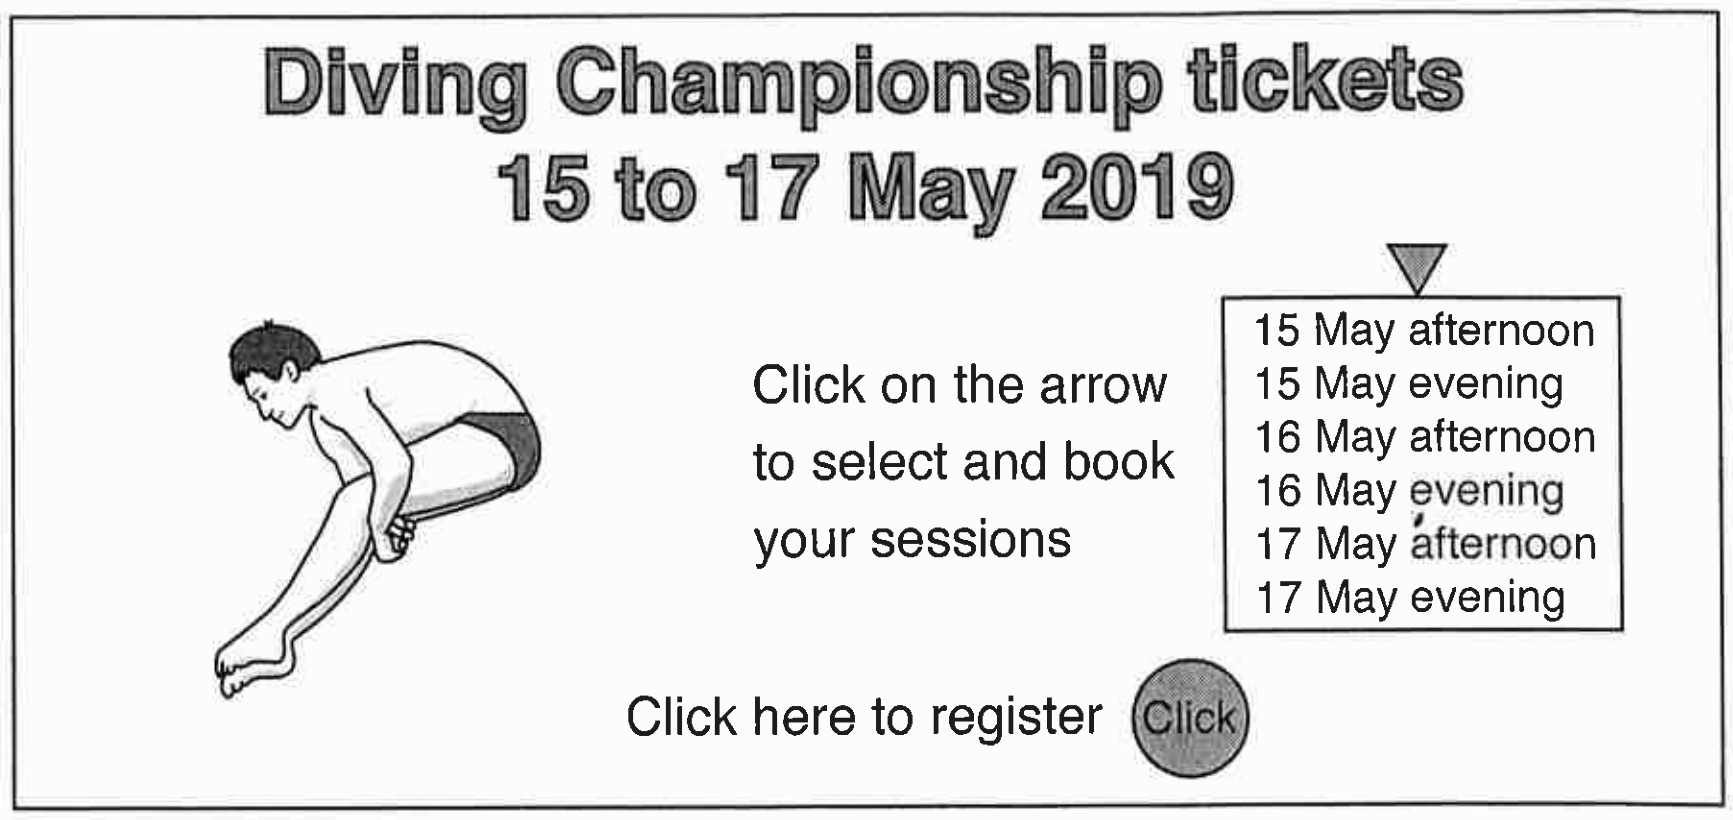
\includegraphics[width=0.5\paperwidth]{C:/Users/Admin/Desktop/Github/question_bank/LyX/static/img/9597-ALVL-2018-P2-Q6-1}
\par\end{center}
\begin{enumerate}
\item State the type of user interface that the ticket ordering website
uses. \hfill{}{[}1{]}
\item All ticket sales are stored on a database server in the following
tables: 

\texttt{CUSTOMER(}\texttt{\uline{CustomerID}}\texttt{, CustomerName,
Email, ContactNumber) }

\texttt{BOOKING(}\texttt{\uline{BookinoID}}\texttt{, BookingDate,
CustomerID) }

\texttt{SESSION(}\texttt{\uline{SessionID}}\texttt{, Date, Time,
SessionCost) }

\texttt{BOOKING\_SESSION(}\texttt{\uline{BookingID}}\texttt{, }\texttt{\uline{SessionID}}\texttt{,
Quantity)} 

\texttt{CustomerID} is the unique identifier in the \texttt{CUSTOMER}
table. 

\texttt{BookingID} is the unique identifier in the \texttt{BOOKING}
table. 

\texttt{SessionID} is the unique identifier in the \texttt{SESSION}
table. 
\begin{enumerate}
\item Draw an Entity-Relationship (E-R) diagram to represent this data model.
\hfill{}{[}4{]}
\item Name the fields that would be used to calculate the customer\textquoteright s
payment for a session. \hfill{}{[}2{]}
\end{enumerate}
\item Before customers can make an online ticket purchase, they have to
fill in a registration form. The details from this form are used to
complete the CUSTOMER table. 
\begin{center}
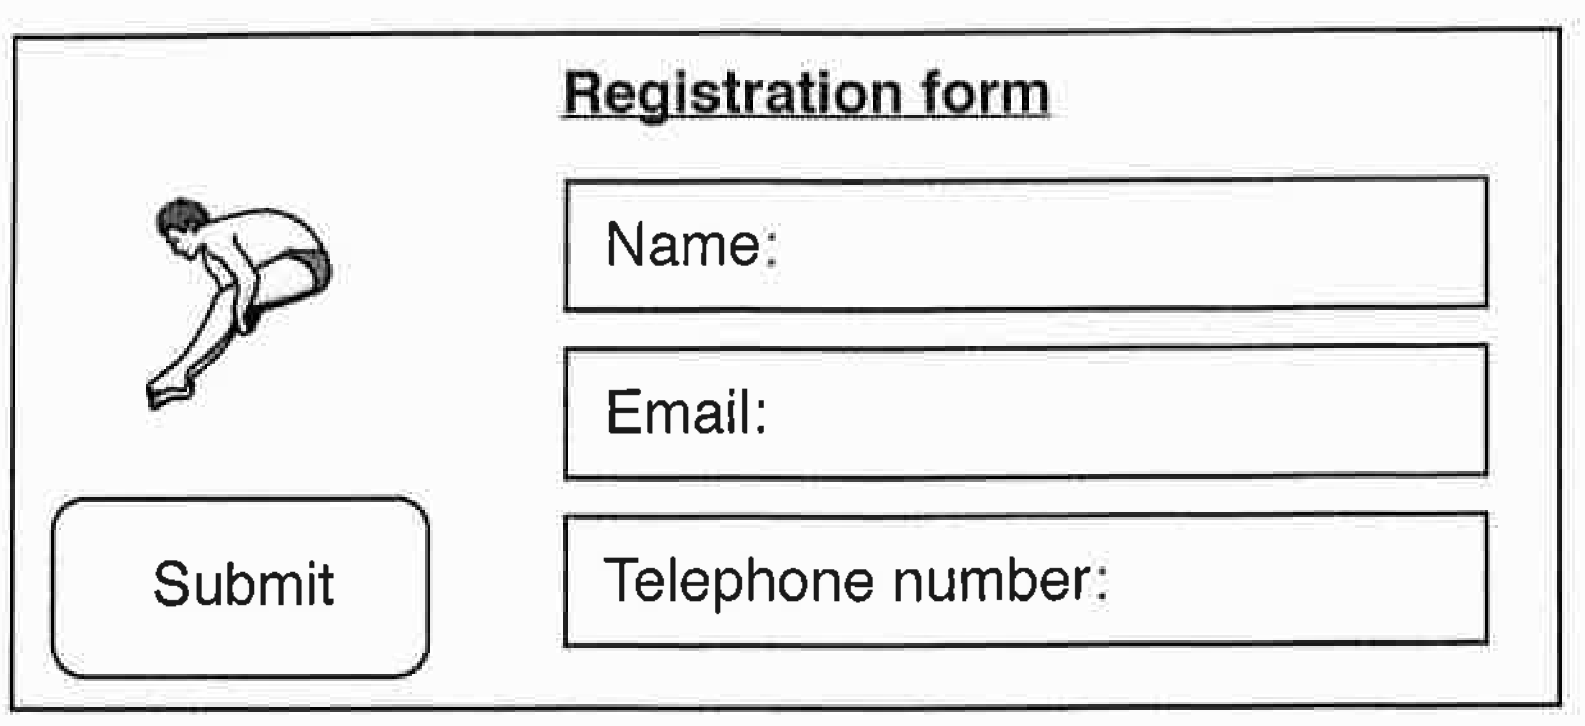
\includegraphics[width=0.5\paperwidth]{C:/Users/Admin/Desktop/Github/question_bank/LyX/static/img/9597-ALVL-2018-P2-Q6-2}
\par\end{center}

Explain how the web server will use server-side script to process
this form. \hfill{} {[}5{]}
\item The organisers of the championship store all the data for the event
using cloud storage. 

Describe\textbf{ three} economic benefits to the organisers of using
cloud-based storage. \hfill{}{[}3{]}
\end{enumerate}

 \newpage 

\item \textbf{{[}ALVL/9597/2019/P1/Q1{]} }

A text file, \texttt{TIDES.TXT}. contains the low and high tide information
for a coastal location tor each day of a month. Each line contains
tab-delimited data that shows the date, the time. whether the tide
is high or low and the tide height in metres. 

Each line is in the format: 
\begin{center}
\texttt{YYYY-MM-DD\textbackslash tHH:mm\textbackslash tTIDE\textbackslash tHEIGHT\textbackslash n }
\par\end{center}
\begin{itemize}
\item The date is in the term YYYY-MM-DD, for example. 2019-08-03 is 3rd
August. 2019 
\item The time is in the form HH:mm, for example. 13:47 
\item TIDE is either HIGH or LOW 
\item HEIGHT is a positive number shown to one decimal place 
\item \texttt{\textbackslash t} represents the tab character
\item \texttt{\textbackslash n} represents the newline character 
\end{itemize}
The text file is stored in ascending order of date and time.

\subsubsection*{Task 1.1}

Write program code to:
\begin{itemize}
\item read the tide data from a text file
\item find the highest high tide and print this value
\item find the lowest low tide and print this value.
\end{itemize}
Use \texttt{TIDES.TXT} to test your program code.

\subsubsection*{Evidence 1}

Your program code.

Screenshot of your output. \hfill{}{[}9{]} 

\subsubsection*{Task 1.2}

The tidal range is the difference between the heights of successive
tides; from a high tide to the following low tide or from a low tide
to the following high tide.

Amend your program code to:
\begin{itemize}
\item output the largest tidal range and the date on which the second tide
occurs
\item output the smallest tidal range and the date on which the second tide
occurs.
\end{itemize}
Use \texttt{TIDES.TXT} to test your program code.

\subsubsection*{Evidence 2}

Your program code.

Screenshot of your output. \hfill{}{[}9{]}

 \newpage 

\item \textbf{{[}ALVL/9597/2019/P1/Q2{]} }

Characters are numerically encoded using ASCII codes.
\begin{itemize}
\item 'A' has the denary value 65; \textquoteleft B' has the denary value
66 and so on.
\item 'a' has the denary value 97; 'b' has the denary value 98 and so on.
\end{itemize}
The ROT-13 encoding function replaces a letter with the letter that
is 13 positions after it in the alphabet. Characters that are not
letters remain unchanged. .

The function wraps around from the end of the alphabet back to the
beginning. The case of the coded letter should match the case of the
original letter.

For example:
\begin{itemize}
\item 'A' is replaced with 'N'; 'a' is replaced with 'n'
\item 'B' is replaced with '0\textquoteleft ; 'b' is replaced with 'o' 
\item 'Z' is replaced with 'M'; 'z\textquoteleft{} is replaced with 'm'
\end{itemize}

\subsubsection*{Task 2.1}

Write program code that:
\begin{itemize}
\item reads a string of characters as input
\item encodes the string in ROT-13 form
\item outputs the encoded string.
\end{itemize}
Run the program \textbf{three} times with the inputs: 

\noindent\begin{minipage}[t]{1\columnwidth}%
\texttt{This is a word.}

\texttt{ALL \&\&\&\& CAPITALS}

\texttt{UpperCamelCase12()}%
\end{minipage}

\subsubsection*{Evidence 3}

Your program code.

Screenshots of your outputs. \hfill{}{[}9{]}

\subsubsection*{Task 2.2}

A string is encoded using ROT-13. The resulting string is then encoded
using ROT-13. The output of the second encoding should be identical
to the original string.

Amend your program code to apply HOT-13 twice, in the method described.
Show that the resulting string is identical to the original string.

\subsubsection*{Evidence 4}

Your program code.

Screenshot of the output from one of the given inputs. \hfill{}{[}3{]}

 \newpage 

\item \textbf{{[}ALVL/9597/2019/P1/Q3{]} }

A program is to be written to implement a to-do list using object-oriented
programming (OOP). The list shows tasks that need to be done.

Each task is given a category and a description.

The base class will be called \texttt{ToDo} and is designed as follows: 
\begin{center}
\begin{tabular}{|l|}
\hline 
\texttt{\hspace{0.25\columnwidth}ToDo}\tabularnewline
\hline 
\texttt{category : STRING }\tabularnewline
\texttt{description : STRING}\tabularnewline
\hline 
\texttt{constructor(c : STRING, d : STRING) }\tabularnewline
\texttt{set\_category(s : STRING)}\tabularnewline
\texttt{set\_description(s : STRING) }\tabularnewline
\texttt{get\_category() : STRING }\tabularnewline
\texttt{get:\_description() : STRING }\tabularnewline
\texttt{summary() : STRING}\tabularnewline
\hline 
\end{tabular}
\par\end{center}

The \texttt{summary()} method returns the category and description
as a single string.

\subsubsection*{Task 3.1}

Write program code to define the class \texttt{ToDo}.

\subsubsection*{Evidence 5}

Your program code. \hfill{}{[}5{]}

Tasks should be sorted alphabetically by category. Within each category.
tasks should be sorted alphabetically by description. 

A task to be added to the list is compared to the tasks already in
the list to determine its correct position in the list. If the list
is empty. it is added to the beginning of the list. 

This comparison will use an additional member method,
\begin{center}
\texttt{compare\_with(td : ToDo) : INTEGER }
\par\end{center}

This function compares the instance (the item in the list) and the
\texttt{ToDo} object passed to it, returning one of three values:

\texttt{\qquad{}}-1 if the instance is before the given \texttt{ToDo}

\texttt{\qquad{}}0 if the two are equal

\texttt{\qquad{}}+1 if the instance is after the given \texttt{ToDo}

\subsubsection*{Task 3.2}

There are four objects defined in the text file \texttt{TASK3\_2.TXT}.

Write program code to:
\begin{itemize}
\item implement the \texttt{compare\_with()} method
\item create an empty list of \texttt{ToDo} objects
\item add each of the four objects in the text file \texttt{TASK3\_2.TXT}
to its appropriate place in the list
\item printout the list contents using the \texttt{summary()} method.
\end{itemize}

\subsubsection*{Evidence 6}

Your program code.

Screenshot of test run. \hfill{}{[}13{]}

The to-do list can have items with extra information. One such item
has a date by which the task should be completed. 

The \texttt{DatedToDo} class inherits from the \texttt{ToDo} class,
extending it to have a \texttt{due\_date}. designed as follows: 
\begin{center}
\begin{tabular}{|l|}
\hline 
\hspace{0.25\columnwidth}DatedToDo : ToDo\tabularnewline
\hline 
\texttt{due\_date : DATE}\tabularnewline
\hline 
\texttt{constructor(dt : DATE, 0 : STRING, d : STRING)}\tabularnewline
\texttt{set\_due\_date(d : DATE)}\tabularnewline
\texttt{get\_due\_date() : DATE }\tabularnewline
\hline 
\end{tabular}
\par\end{center}

The \texttt{DatedToDo} class should extend the \texttt{compare\_with()}
method to ensure that tasks are ordered by ascending \texttt{due\_date},
and then by the ordering used by the base \texttt{compare\_with()}
method. The \texttt{summary()} method should also be extended to return
the \texttt{due\_date} and the return values of the base \texttt{summary()}
method.

\subsubsection*{Task 3.3}

There are seven objects defined in the text file \texttt{TASK3\_3.TXT}.

Amend your program code to:
\begin{itemize}
\item implement the \texttt{DatedToDo} class, with \texttt{constructor},
\texttt{get\_due\_date} and \texttt{set\_due\_date}
\item implement the extended \texttt{compare\_with()} method
\item implement the extended \texttt{summary()} method
\item ensure all seven objects in the text file \texttt{TASK3\_3.TXT} are
added to the list
\item print out the list contents using the \texttt{summary()} method.
\end{itemize}

\subsubsection*{Evidence 7}

Your program code. 

Screenshot of the test run.\hfill{}{[}5{]}

\noindent When a task in the to-do list has been completed, it should
be removed.

\subsubsection*{Task 3.4}

There are four completed tasks defined in the text file \texttt{TASK3\_4.TXT}.

If any of the four tasks exists in the list, it should be removed.

Amend your program to: 
\begin{itemize}
\item recreate the list of seven tasks from Task 3.3
\item check if each of the four completed tasks in the text file \texttt{TASK3\_4.TXT}
exists in the list and: 
\begin{itemize}
\item remove it from the list if it does or 
\item print a warning message it the completed task does not exist
\end{itemize}
\item print out the list after all four objects have been processed. 
\end{itemize}

\subsubsection*{Evidence 8}

Your amended code.

Screenshot of the test run.\hfill{}{[}10{]}

 \newpage 

\item \textbf{{[}ALVL/9597/2019/P1/Q4{]} }

A stack is used to store characters.

\subsubsection*{Task 4.1}

Write program code to implement the stack and the operations specified.

Your code should allow operations to: 
\begin{itemize}
\item push an item on to the stack
\item pop an item off the stack
\item determine the size of the stack. A size of zero indicates that the
stack is empty.
\end{itemize}

\subsubsection*{Evidence 9}

Your program code for the stack.\hfill{}{[}10{]}

The stack is to be used to identify it an arithmetic expression is
balanced. 

An expression is balanced if each opening bracket has a corresponding
closing bracket. 

Different pairs of brackets can be used. These are: {[}{]}, () or
\{\}. 

This is an example of an expression that is balanced.

\texttt{\qquad{}({[}8-1{]}/(5{*}7)) }

This is an example of an expression that is not balanced. 

\texttt{\qquad{}{[}(8-1{]}/(5{*}7)) }

Note the change in the order of the first two open bracket symbols.
The first closing bracket should be a closing bracket ')' to match
the previous opening bracket \textquoteleft ('. 

Note that an expression is not balanced if the order of the brackets
is incorrect, even if there are the same number of opening and closing
brackets of each bracket type. 

An expression is checked by iterating over it: 
\begin{itemize}
\item if a non-bracket symbol is found, continue to the next character. 
\item If an opening symbol is found, push it on to the stack and continue
to the next character. 
\item If a closing bracket is encountered: 
\begin{itemize}
\item If the stack is empty, return an error (because there is no corresponding
opening bracket) 
\item else pop the symbol from the top of the stack and compare it to the
current closing symbol to see if they make a matching pair 
\item If they do match continue to the next character 
\item else return an error (pairs of brackets must match). 
\end{itemize}
\item When the last symbol is encountered: 
\begin{itemize}
\item return an error if the stack is not empty (too many opening symbols) 
\item else return a success message.
\end{itemize}
\end{itemize}

\subsubsection*{Task 4.2}

Add \textbf{five} other suitable test cases and a reason for choosing
each test case.
\begin{center}
\begin{tabular}{|l|l|l|}
\hline 
\hspace{0.05\columnwidth}\textbf{Test case} & \textbf{Reason for choice} & \textbf{Expected value}\tabularnewline
\hline 
\texttt{({[}8-1{]}/(5{*}7))} & Provided & Succeeds\tabularnewline
\hline 
\texttt{{[}(8-1{]}/(5{*}7))} & Provided & Fails\tabularnewline
\hline 
 &  & Succeeds\tabularnewline
\hline 
 &  & Succeeds\tabularnewline
\hline 
 &  & Fails\tabularnewline
\hline 
 &  & Fails\tabularnewline
\hline 
 &  & Fails\tabularnewline
\hline 
\end{tabular}
\par\end{center}

\subsubsection*{Evidence 10}

The completed table with all seven test cases and a reason for choosing
each test case.\hfill{}{[}6{]}

\subsubsection*{Task 4.3}

Write program code that checks expressions using the given algorithm. 

Use all \textbf{seven} test cases to verify It.

\subsubsection*{Evidence 11}

Your program code for the stack.

Screenshots for each test data run. \hfill{}{[}19{]}

 \newpage 

\item \textbf{{[}ALVL/9597/2019/P2/Q1{]} }

Pharmacists working in a group of pharmacies, dispense medicine to
patients who present to them a prescription written by a doctor. A
new system is to be built to allow a doctor to send prescription data
electronically to a pharmacy of the patient's choice. Patients will
either collect the medicine, or have the pharmacy deliver it to them. 

A project proposal is written and sent to doctors and pharmacy staff,
inviting each to respond within a given time. 
\begin{enumerate}
\item Give a reason why the project proposal is sent to: 
\begin{enumerate}
\item Doctors \hfill{}{[}1{]}
\item Pharmacy staff \hfill{}{[}1{]}
\end{enumerate}
\end{enumerate}
The responses from the doctors and pharmacy staff are reviewed. Invitations
are sent to doctors to find out whether they are willing to take part
in a pilot scheme. The project proposal is sent to prospective software
developers. Some of the activities involved in the project are listed
in the following table. 
\begin{center}
\begin{tabular}{|c|l|c|}
\hline 
Label & \hspace{0.25\columnwidth}Activity & Duration(Weeks)\tabularnewline
\hline 
\textbf{A} & Send project proposal  & 4\tabularnewline
\hline 
\textbf{B} & Send project proposal to pharmacy staff & 2\tabularnewline
\hline 
\textbf{C} & Discuss all the responses from A and B. and revise the proposal if
2 required & 2\tabularnewline
\hline 
\textbf{D} & Send project proposal to prospective software developers & 3\tabularnewline
\hline 
\textbf{E} & Invite doctors to be part of a pilot scheme & 2\tabularnewline
\hline 
\textbf{F} & Request quotations of cost and development time from software developers & 3\tabularnewline
\hline 
\textbf{G} & Select a software developer  & 1\tabularnewline
\hline 
\end{tabular}
\par\end{center}
\begin{enumerate}
\item[(b)] {}
\begin{enumerate}
\item Draw a Gantt chart for the activities labelled \textbf{A} to \textbf{G}.
\hfill{}{[}6{]}
\item State the estimated time taken to complete activities \textbf{A} to
\textbf{G}. \hfill{}{[}1{]}
\end{enumerate}
\end{enumerate}
In activities \textbf{A} and \textbf{B}, doctors and pharmacy staff
identified ethical and security issues that would need to be addressed. 
\begin{enumerate}
\item[(c)] {}
\begin{enumerate}
\item Describe one security issue. \hfill{}{[}2{]}
\item Describe one ethical issue. \hfill{}{[}2{]}
\end{enumerate}
\end{enumerate}
In activity \textbf{F}, quotations are received from software developers.
The lowest cost is from a developer who works alone, but demonstrates
a number of successful projects. Other software developers that employ
many staff submit more expensive quotations. 
\begin{enumerate}
\item[(d)] Explain why the group of pharmacies may decide against the single
developer. \hfill{}{[}2{]}
\end{enumerate}
An analyst from the chosen software developer reviews the current
system. 
\begin{enumerate}
\item[(e)] Give \textbf{four} methods available to the analyst to find out how
a system operates. \hfill{}{[}4{]}
\end{enumerate}
The analyst proposes that the doctors and pharmacy staff interact
with a web-based system. 
\begin{enumerate}
\item[(f)] tate the software that will be needed on the devices used by the
doctors and pharmacy staff. other than the operating system. \hfill{}{[}1{]}
\end{enumerate}
The alternative to a web-based system would be to write and install
purpose-built application software for each computer used by a doctor
or member of the pharmacy staff. 
\begin{enumerate}
\item[(g)] Describe \textbf{two} advantages to the software developer of a web-based
solution over purpose- built software running on each user's computer.
\hfill{}{[}4{]}
\end{enumerate}
Doctors may wish to write prescriptions when they visit patients in
their own home. 
\begin{enumerate}
\item[(h)] Explain \textbf{one} benefit of a web-based solution in this situation.
\hfill{}{[}2{]}
\end{enumerate}
The computers used by the doctors and pharmacy staff are clients of
the server operated by the pharmacy. Some validation is provided by
client-side scripting.
\begin{enumerate}
\item[(i)] Give \textbf{two} advantages of using this type of scripting. \hfill{}{[}2{]}
\end{enumerate}
The new system is designed. coded and tested as a number of modules.
A tester performing black-box testing on a module would need its specification. 
\begin{enumerate}
\item[(j)] Explain why the tester would not need access to the source code.
\hfill{}{[}2{]}
\item[(k)] Explain why someone designing a test strategy for white box testing
would need access to the source code. \hfill{}{[}2{]}
\item[(l)] Alpha testing is performed on the system. 

Explain the purpose of alpha testing. \hfill{} {[}2{]}
\item[(m)] The group of pharmacies is responsible for the security and integrity
of the stored data. 
\begin{enumerate}
\item Give \textbf{two }methods that could be used to ensure security of
the stored data. \hfill{}{[}2{]}
\item Give \textbf{two} methods that could be used to ensure the integrity
of the stored data. \hfill{}{[}2{]}
\end{enumerate}
\item[(n)] The group considers using either the cloud or its own server to store
data needed by the proposed system. 

Give \textbf{one} advantage and \textbf{one} disadvantage of storing
the data in the cloud. \hfill{}{[}2{]}
\end{enumerate}

 \newpage 

\item \textbf{{[}ALVL/9597/2019/P2/Q2{]} }

A bakery bakes bread and cakes to sell in its own shop and to other
shops throughout a city. 

Its drivers visit every shop each day, delivering that day\textquoteright s
order and collecting the order for the next day. 

Order forms are pre-printed with the name of each shop and every item
that the bakery bakes. The manager of each shop writes onto the form
the quantity of each item required. When the drivers return to the
bakery. the data from the order forms are collated to give the bakers
the total of each item to bake. 

Copies of the order forms are made and used as delivery notes for
the next day\textquoteright s deliveries. The accounts department
use the original order forms to prepare a weekly invoice for each
shop.

The bakery wants the shops to submit their orders online. 

A program is needed to determine the number of each item needed and
produce the weekly invoice for each shop.

The new program will use a relational database with three tables:
Product, Shop and Order. 

Each product has a description. price. and a unique product ID number. 

Each shop has a name. an address, telephone number. manager's name,
and a unique shop iD number. 

Each order has a product lD, a quantity, a shop ID and a date for
delivery. 
\begin{enumerate}
\item Draw an Entity-Relationship (E-R) diagram showing the three tables
and the relationships between them. \hfill{}{[}5{]}
\item A table description can be expressed as: 

\texttt{TableName (}\texttt{\uline{Attribute1}}\texttt{, Attribute2,
Attribute3, ...) }

The primary key is indicated by underlining one or more attributes. 

Write table descriptions for the three tables. \hfill{}{[}4{]}
\end{enumerate}
The bakery can change the price of an item at any time. Validation
ensures that the new price is within specified limits and is more
likely to be correct.
\begin{enumerate}
\item[(c)] {}
\begin{enumerate}
\item Explain why this could still result in incorrect weekly invoices,
assuming that the new price input is correct. \hfill{}{[}2{]}
\item Describe changes to the database and draw a modified E-R diagram to
ensure correct invoices are created. \hfill{}{[}4{]}
\end{enumerate}
\end{enumerate}

 \newpage 

\item \textbf{{[}ALVL/9597/2019/P2/Q3{]} }

A programmer is asked to write a program to store names in alphabetical
order.

The program needs to:
\begin{itemize}
\item add and remove names
\item search for the presence of a specific name
\item output all the names in alphabetical order. 
\end{itemize}
The programmer considers two options: an array and a linked list.
\begin{enumerate}
\item {}
\begin{enumerate}
\item Explain why an array allows for more efficient searching. \hfill{}{[}2{]}
\item State why this advantage becomes more significant as the number of
names becomes much larger. \hfill{}{[}1{]}
\end{enumerate}
\item {}
\begin{enumerate}
\item Give \textbf{one} disadvantage of using an \textbf{array} to store
the names in alphabetical order. \hfill{}{[}2{]}
\item Give \textbf{one} advantage of using a \textbf{linked list} to store
the names in alphabetical order. \hfill{}{[}2{]}
\end{enumerate}
\end{enumerate}
A third option is to store the names in a binary tree.
\begin{enumerate}
\item[(c)] Explain how a binary tree provides some of the advantages of both
an array and a linked list when storing sorted data. \hfill{}{[}2{]}
\item[(d)] State why a binary tree may need to be re-created with exactly the
same data items. \hfill{}{[}1{]}
\end{enumerate}

 \newpage 

\item \textbf{{[}ALVL/9597/2019/P2/Q4{]} }

A company operates a multi-storey car park. All parking bays are identified
by a letter. indicating the floor. and a number indicating the position
of the bay on that floor (for example. C34 indicates bay 34 on floor
C). 

The entrance to the car park is controlled by a barrier. Before the
barrier lifts to allow a car to enter, the driver must press a button
to indicate if they need a standard bay or a special bay. 

Special bay users must present a card to a card reader at the barrier. 

The car park has an additional third type of bay that has a charging
point for electric vehicles. The hourly rate for these bays is not
the same as standard bays. The cost of using this type of bay additionally
depends on the cost of the electricity used. This is monitored by
the charging device and stored.

A camera captures the vehicle registration number. A ticket is printed
showing:
\begin{itemize}
\item current time
\item vehicle registration number 
\item floor letter 
\item position number of a suitable bay where the car must be parked 
\item the card number for the special bay, if a card had been presented
at the barrier. 
\end{itemize}
When the driver takes the ticket from the printer. the entrance barrier
lifts. Before a car is allowed to leave, the ticket must be presented
and a charge paid. The charge is determined by the length of stay
and type of bay. The hourly rate for a standard bay is not the same
as that for a special bay. As a car approaches the exit barrier a
camera captures the vehicle registration. The barrier only lifts if
the charge for this vehicle has been paid. 

This system is to be implemented using object-oriented programming
(OOP). 

The base class PARKING\_BAY has a property to store whether or not
a bay is occupied. 
\begin{enumerate}
\item Draw a class diagram, showing:
\begin{itemize}
\item any derived classes and inheritance from the base class
\item the properties needed in the base, and any derived classes
\item suitable methods to support the system with at least one getter and
one setter method. \hfill{}{[}8{]}
\end{itemize}
\item Add a class, CAR\_PARK. thathas properties to store:
\begin{itemize}
\item a list of all bays
\item the number of unoccupied bays. \hfill{}{[}3{]}
\end{itemize}
\item Explain why polymorphism is useful in object-oriented programming.
\hfill{}{[}2{]}
\item Explain the purpose of making the attributes of an object private.
\hfill{}{[}2{]}
\end{enumerate}

 \newpage 

\item \textbf{{[}ALVL/9597/2019/P2/Q5{]} }

The function \texttt{z} takes three integer parameters, \texttt{low},
\texttt{high}, \texttt{seek} and returns an integer value. It operates
on the values in the elements of the array \texttt{A}. 

\noindent %
\noindent\begin{minipage}[t]{1\columnwidth}%
\texttt{01 FUNCTION Z(low, high, seek, A) RETURNS INTEGER }

\texttt{02 \qquad{}IF low > high THEN }

\texttt{03 \qquad{}\qquad{}RETURN \textemdash 1 }

\texttt{04 \qquad{}ENDIF }

\texttt{05 \qquad{}mid <- low + INT( (high \textemdash{} low) /2)}

\texttt{06 \qquad{}IF seek = A{[}mid{]} THEN}

\texttt{07 \qquad{}\qquad{}RETURN mid }

\texttt{08 \qquad{}ELSE }

\texttt{09 \qquad{}\qquad{}IF seek < A{[}mid{]} THEN }

\texttt{10 \qquad{}\qquad{}\qquad{}RETURN Z(low, mid - 1, seek,
A) }

\texttt{11 \qquad{}\qquad{}ELSE }

\texttt{12 \qquad{}\qquad{}\qquad{}RETURN Z(mid + 1, high, seek,
A) . }

\texttt{13 \qquad{}\qquad{}ENDIF }

\texttt{14 \qquad{}ENDIF }

\texttt{15 ENDFUNCTION}%
\end{minipage}
\begin{enumerate}
\item {}
\begin{enumerate}
\item State what lines \texttt{10} and \texttt{12} tell you about the function.
\hfill{}{[}1{]}
\item State the purpose for the \texttt{RETURN} statements in lines \texttt{03}
and \texttt{07} of function \texttt{z}. \hfill{} {[}1{]}
\end{enumerate}
\end{enumerate}
The values in each of the eight elements of the array \texttt{A} are:
\begin{center}
\begin{tabular}{|l|c|c|c|c|c|c|c|c|}
\multicolumn{1}{l}{\textbf{Element}} & \multicolumn{1}{c}{0} & \multicolumn{1}{c}{1} & \multicolumn{1}{c}{2} & \multicolumn{1}{c}{3} & \multicolumn{1}{c}{4} & \multicolumn{1}{c}{5} & \multicolumn{1}{c}{6} & \multicolumn{1}{c}{7}\tabularnewline
\hline 
\textbf{Value} & -3 & 8 & 14 & 15 & 96 & 101 & 412 & 500\tabularnewline
\hline 
\end{tabular}
\par\end{center}
\begin{enumerate}
\item Copy and then complete the trace table for the instruction: 

\texttt{OUTPUT z(0, 7, 103, A)}
\begin{center}
\begin{tabular}{|c|c|c|c|c|c|c|}
\hline 
Function call & \texttt{\textbf{low}} & \texttt{\textbf{high}} & \texttt{\textbf{seek}} & \texttt{\textbf{mid}} & \texttt{\textbf{A{[}mid{]}}} & \texttt{\textbf{OUTPUT}}\tabularnewline
\hline 
\texttt{1} & \texttt{0} & \texttt{7} & \texttt{103} &  &  & \tabularnewline
\hline 
 &  &  &  &  &  & \tabularnewline
\hline 
 &  &  &  &  &  & \tabularnewline
\hline 
 &  &  &  &  &  & \tabularnewline
\hline 
 &  &  &  &  &  & \tabularnewline
\hline 
 &  &  &  &  &  & \tabularnewline
\hline 
\end{tabular}
\par\end{center}

\hfill{}{[}4{]}
\item Function \texttt{z} can return two different types of value.

Explain what these represent. \hfill{}{[}2{]}
\item The number of elements in array \texttt{A} may be very large. 

Explain why a programmer might prefer to use an iterative approach
rather than the one used in function \texttt{z}. \hfill{} {[}2{]}
\end{enumerate}

 \newpage 

\item \textbf{{[}ALVL/9597/2019/P2/Q6{]} }

Data communication networks can use circuit switching or packet switching. 
\begin{enumerate}
\item {}
\begin{enumerate}
\item Give \textbf{two} advantages of packet switching over circuit switching.
\hfill{}{[}2{]}
\item Give \textbf{one} advantage of circuit switching over packet switching.
\hfill{}{[}1{]}
\end{enumerate}
\item {} 
\begin{enumerate}
\item State \textbf{one} reason for using either a parity check or a checksum.
\hfill{}{[}1{]}
\item Give \textbf{one} example of an error that a parity check cannot detect.
\hfill{}{[}1{]}
\end{enumerate}
\item Switches and routers are common devices used in networking. 

Explain the most significant differences between a switch and a router.
\hfill{}{[}2{]}
\item Explain the purpose of a bridge in a network.\hfill{}{[}1{]}
\item A local area network (LAN) can be set up as either client-server or
peer-to-peer. 

Give \textbf{two} advantages in storing shared data on a client-server
network rather than on a peer-to-peer network. \hfill{}{[}2{]}
\end{enumerate}

 \newpage 



 \end{enumerate}

 \end{document}

